\documentclass[oneside]{mgr}
\usepackage[section] {placeins}


\usepackage{polski}      
\usepackage[utf8]{inputenc} 
\usepackage[T1]{fontenc} 
\usepackage{graphicx}
\usepackage{subfigure}
\usepackage{psfrag}
\usepackage{amsmath}
\usepackage{amsfonts}
\usepackage{supertabular}
\usepackage{array}
\usepackage{tabularx}
\usepackage{hhline}

\usepackage{showlabels}% w finalnej do usuniecia
\newcommand{\R}{I\!\!R} 
\newtheorem{theorem}{Twierdzenie}[section] 
\title{Wybór cech do rozpoznawania \\złożonych form przestrzennych}
\engtitle{Selection of features \\for recognizing complicated shapes}
\author{inż. Jan Słowik}
\supervisor{Prof. dr hab. inż. Ewaryst Rafajłowicz, I-6}
\date{2012} 
\field{Informatyka (INF)} 
\specialisation{Inżynieria systemów informatycznych (INS)}
\begin{document}
\bibliographystyle{plabbrv} 
\maketitle 
\dedication{6cm}{Dedykuję moim rodzicom.}
\tableofcontents 

\chapter{Wstęp}
Widzenie maszynowe jest podzbiorem szerokiej dziedziny informatyki jaką jest przetwarzanie obrazów. W ostatnich latach nauka ta dynamicznie się rozwija wraz ze wzrostem mocy obliczeniowej. W ramach widzenia maszynowego niezwykle ciekawym zagadnieniem jest rozpoznawanie obrazów. 

Samo zadanie rozpoznawania obrazów, nie jest z punktu widzenia sztucznej inteligencji dużym problem. Aby móc rozpoznawać obrazy należy posiadać zbiór cech według których będziemy klasyfikować. Przetwarzanie obrazów rozumiane jako filtracja i analiza, mające na celu opracowanie zbioru cech obrazu jest najbardziej złożonym  i skomplikowanym procesem. 

Początki widzenia maszynowego znajdują się w przemyśle, gdzie systemy wizyjne były i są wykorzystywane do nadzorowania procesów produkcyjnych. Odbywa się to w ściśle określonych i zoptymalizowanych dla konkretnego systemu warunkach działania. W raz rozwojem innych dziedzin informatyki takich jak np. rozszerzona rzeczywistość czy robotyka, widzeniu maszynowego stawiane są coraz to nowe wyzwania. Są to np. jak praca w zmiennej orientacji, w zróżnicowanym środowisku w dowolnych warunkach. Wymusza to poszukiwanie nowych rozwiązań wykrywających cechy charakterystyczne obiektów. Cechy takie powinny być możliwie jak najmniej zależne od transformacji takich jak skalowanie i rotacja obrazu,lokalizacji kamery oraz odporne na zmienne oświetlenie obiektu. 

Celem badawczym niniejszej pracy było przebadanie 6 algorytmów służących do ekstrakcji i opisu cech obrazów. Algorytmy te zostały przetestowane pod kątem skuteczności jak i szybkości działania. Ponadto podjęto prace mające na celu opracowanie hybrydowego algorytmu będącego syntezą wcześniej opisanych metod metod. Jako przykład skomplikowanych form przestrzennych zdecydowano się część testów wykonać na obrazach przedstawiających formacje skalne.
\part{Teoria}
\chapter{Przegląd algorytmów wyszukujących cechy obrazów}
Poszukując algorytmów służących do lokalizowania cech charakterystycznych obrazów posłużono się badaniami \cite{IK111}, \cite{IK112}. Autor w oparciu o prace \cite{LIFDAS} dokonał zestawienia popularnych metod zaimplementowanych w służacych do przetwarzania obrazów bibliotece OpenCV (\textit{wersje 2.2.0 i 2.3.1}). Algorytmy były testowane testowym zbiorze obrazów przedstawionym na rysunku \ref{fig:zestaw_obrazow_start}, a wyniki badań prezentują rezultaty od \ref{fig:Number-of-detected-features_thumb}, do \ref{fig:Percent-of-tracked-feature_thumb}.

\begin{figure}[!htb]
\begin{center}

\subfigure[Barbara]{
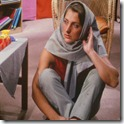
\includegraphics{pict/01/barbara_thumb.jpg}
\label{pict:01_Barbara}
}
\subfigure[Lena]{
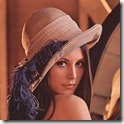
\includegraphics{pict/01/lena_thumb.jpg}
\label{pict:01_Lena}
}
\subfigure[Pepppers]{
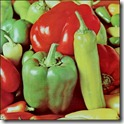
\includegraphics{pict/01/peppers_thumb.jpg}
\label{pict:01_Pepppers}
}
\subfigure[Mandril]{
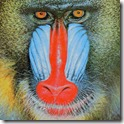
\includegraphics{pict/01/mandril_thumb.jpg}
\label{pict:01_Mandril}
}
\caption{Zestaw obrazów testowych do porównania algorytmów}
\label{fig:zestaw_obrazow_start}
\end{center}
\end{figure}

\begin{figure}[!htb]
\centering
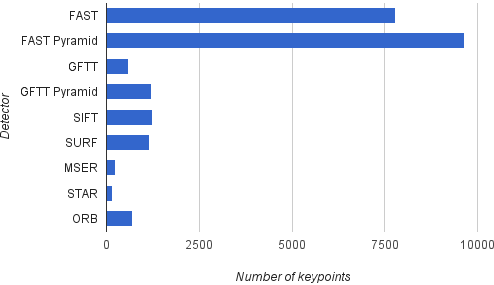
\includegraphics[height=66mm]{pict/01/Number-of-detected-features_thumb.png}
\caption{Liczba wykrytych cech}
\label{fig:Number-of-detected-features_thumb}
\end{figure}

\begin{figure}[!htb]
\centering
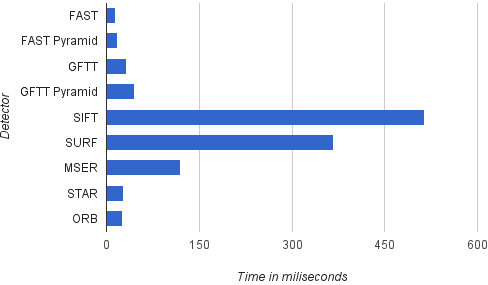
\includegraphics[height=66mm]{pict/01/Detection-cost_thumb.png}
\caption{czas potrzebny na wykrycie cechy}
\label{fig:Detection-cost_thumb}
\end{figure}
\begin{figure}[!htb]
\centering
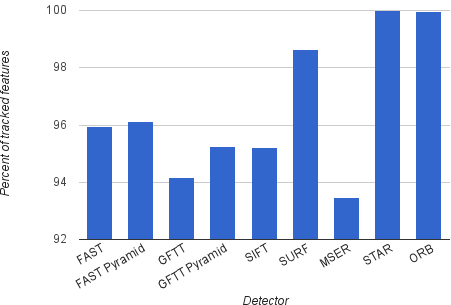
\includegraphics[height=66mm]{pict/01/Percent-of-tracked-feature_thumb.png}
\caption{Skuteczność śledzenia wyszukanych cech}
\label{fig:Percent-of-tracked-feature_thumb}
\end{figure}

\newpage


Na podstawie zaprezentowanych wyników wszystkie algorytmy możemy zaklasyfikować jako dobre, gdyż pozwalają śledzić zlokalizowane cechy z ponad 90 \% skutecznością. Niemniej jednak poszczególne metody różnią się szybkością i ergonomią działania. Algorytm \textbf{FAST} dostarcza bardzo dużą liczbę punktów charakterystycznych w krótkim czasie, ale ze względu na ich stan nie zawsze można je wykorzystać. Algorytmy \textbf{SURF}, \textbf{STAR} i \textbf{ORB} lokalizują mniej cech ale znacznie wyższej klasy. Pośród tych algorytmów przeciętnie wypada algorytm \textbf{SIFT}, który jednak jest jednym z najpopularniejszych i najlepiej udokumentowanych. 

Obrazy skalne są obrazami specyficznymi ze względu na wprowadzającą dużo informacji fakturę skały. Właściwość ta może być przydatna w rozpoznawaniu obiektów jak i stanowić rodzaj szumu zakłócającego pracę algorytmu. Przed dokonaniem eksperymentów nie sposób tego jednoznacznie stwierdzić, a co za tym idzie wybrać optymalną metodę. W związku z powyższym w niniejszej pracy zdecydowano się szczegółowo opisać i przebadać 5 wspomnianych algorytmów reprezentujących różne podejścia.




\newpage
\section{Algorytm SIFT}
Algorytm SIFT (\textit{skrót od Scale Invariant Feature Transform}) został opublikowany w 1999 roku przez Davida G. Lowe \cite{DGL99}. Najpełniejszy jego opis można znaleźć w pracy \cite{DGL04}.  Jest to jeden z najefektywniejszych i szeroko stosowanych algorytmów wyszukiwania charakterystycznych punktów obrazu. Pozwala on lokalizować i opisywać specyficzne cechy obrazu, które są niezależne od transformacji takich jak skalowanie i rotacja, a także w dużym stopniu odporne na zmienne oświetlenie i położenie kamery. Wyszukane punkty kluczowe są dobrze rozpoznawalne zarówno w dziedzinie przestrzennej jak częstotliwościowej. Algorytm ten jest chroniony prawem patentowym.

W działaniu algorytmu możemy wyróżnić 4 etapy przetwarzania:
\begin{enumerate}
\item Detekcja skalo-przestrzennych ekstremów niezależnych od skali i orientacji obrazu.
\item Selekcja punktów charakterystycznych
\item Przypisanie orientacji punktom charakterystycznym
\item Wyliczenie deskryptorów punktów charakterystycznych
\end{enumerate}
\subsection{Detekcja skalo-przestrzennych ekstremów}
\subsubsection{Rozmycie Gaussowskie}
Pierwszym krokiem służącym pozyskaniu punktów charakterystycznych obrazu w jest wygenerowanie jego reprezentacji skalo-przestrzennej (ang. scale-space).  Oryginalny obraz I(x,y) jest poddawany progresywnemu rozmyciu poprzez operację splotu ze jądrem rozmycia gaussowskiego $G(x,y,\sigma)$. W wyniku działania tej operacji otrzymujemy rozmyty obraz $L(x,y,\sigma)$. 
\begin{equation}
L(x,y,\sigma) = G(x,y,\sigma) * I(x,y)
\end{equation}
\begin{equation}
G(x,y,\sigma) = \frac{1}{2\pi\sigma^2}e^{-\frac{x^2+y^2}{2\sigma^2}}
\end{equation}
Jądro rozmycia jest skalowane poprzez współczynnik k. Zwiększając wartość współczynnika k otrzymujemy coraz bardziej rozmyte obrazy. 
\begin{equation}
G(x,y,k\sigma) = \frac{1}{2\pi(k\sigma)^2}e^{-\frac{x^2+y^2}{2(k\sigma)^2}}
\end{equation}
Obrazy rozmyte i oryginalny są grupowane w oktawę. Następnie obraz oryginalny jest próbkowany z 2 razy mniejszą częstotliwością, skutkiem czego  otrzymujemy przeskalowaną, pomniejszoną kopie. Kopia ta podobnie jak oryginał jest poddawana serii progresywnych rozmyć, w wyniku czego otrzymujemy drugą oktawę. Zabiegi te są powtarzane kilkukrotnie. Twórca algorytmu SIFT, David Lowe zaleca utworzenie 4 oktaw, składających się z 5 obrazów.
\begin{figure}[!htb]
\centering
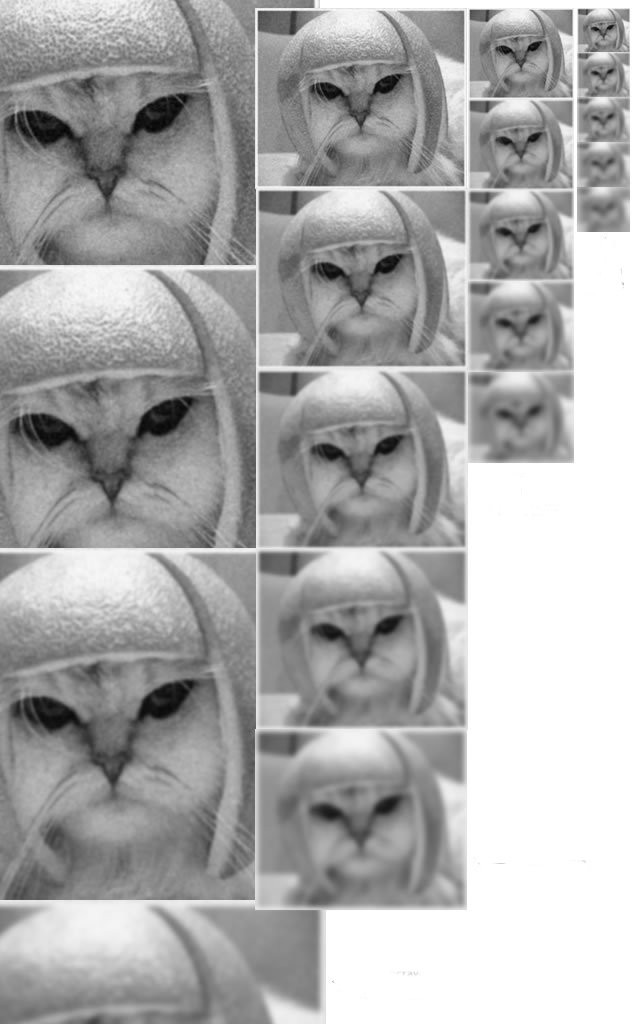
\includegraphics[width=0.8\textwidth]{pict/02/sift/sift_ais_octave.jpg}
\caption{Zestawienie kolejnych oktaw badanego obrazu.}
\label{fig:sift_ais_octave}
\end{figure}

\subsubsection{Różnica Gaussianów}
Kolejnym krokiem jest odjęcie od siebie sąsiadujących obrazów w oktawie. Uzyskane w ten sposób obrazy nazywamy różnicą gausiannów (ang. DoG – Difference  of Gaussian). Z każdej 5 obrazowej oktawy otrzymujemy 4 obrazy różnicowe.
\begin{align}
D(x,y,\sigma) &= (G(x,y,k\sigma)-G(x,y,\sigma))*I(x,y)\\
&= L(x,y,k\sigma) - L(x,y,\sigma)
\end{align}

Różnica gaussianów jest efektywną aproksymacją innej operacji służącej do lokalizowania punktów charakterystycznych – skalowo znormalizowanego Laplasianu Gausjanów $\sigma^2\nabla^2G$ (ang. LoG – Laplacian of Gaussian). Ekstrema LoG dostarczają znacznie bardziej stabilnych punktów charakterystycznych niż detektory takie jak Hessian czy funkcja Harrisa.
\begin{equation}
\frac{\partial G}{\partial \sigma}  = \sigma {\nabla}^2 G
\end{equation}
\begin{equation}
\sigma {\nabla}^2 G = \frac{\partial G}{\partial \sigma} \approx \frac{G(x,y,k\sigma)-G(x,y,\sigma)}{\sigma(k-1)}
\end{equation}

\begin{equation}
G(x,y,k\sigma)-G(x,y,\sigma) \approx (k-1)\sigma^2{\nabla}^2 G
\end{equation}
Aby obliczyć Laplasian Gausjanów należy obraz poddać rozmyciu, a następnie policzyć jego pochodne drugiego stopnia, aby znaleźć lokalne ekstrema. Rozmycie ma na celu redukcje szumów z obrazu, na które bardzo wrażliwe są pochodne drugiego stopnia. W efekcie otrzymujemy stabilne punkty reprezentujące krawędzie i narożniki w obrazie. Mankamentem tej metody jest złożoność obliczeniowa otrzymywania pochodnych drugiego stopnia. Stosując podejście zaproponowane w algorytmie SIFT, duży narzut operacji został zredukowany do prostej subtrakcji obrazów.
\begin{figure}[!htb]
\centering
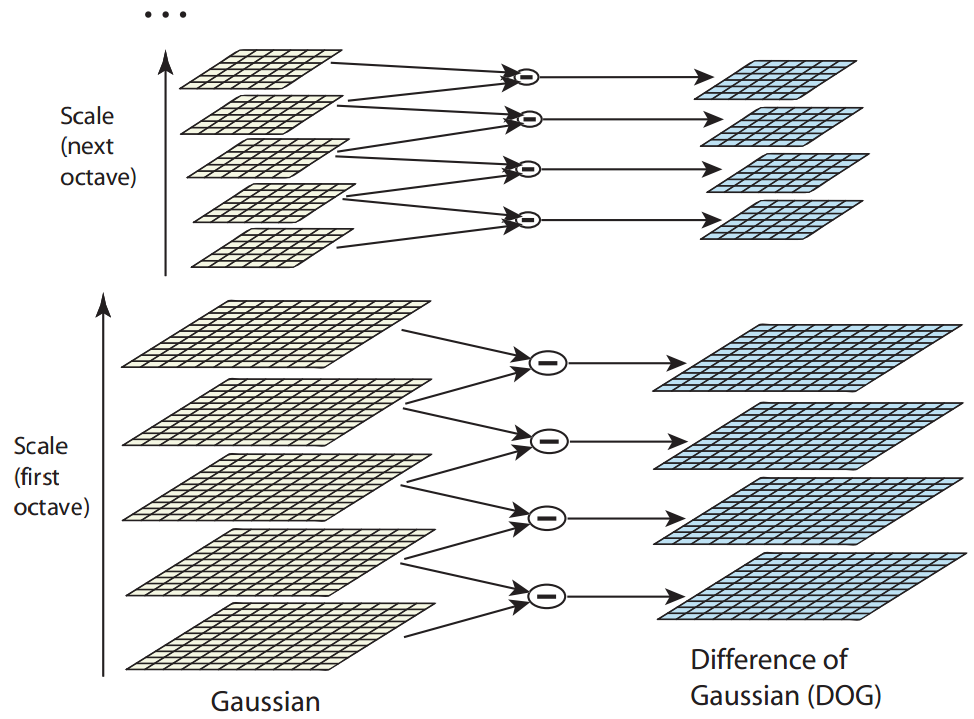
\includegraphics[width=0.8\textwidth]{pict/02/sift/sift_dgl_octave.png}
\caption{Schemat generowania obrazów różnicy Gaussianów}
\label{fig:sift_dgl_octave}
\end{figure}

%ZASTANOWIC SIE CZY COS NAPISAC O MULTIPLIKACJI
\subsubsection{Ekstrema jako potencjalne punkty charakterystyczne}
Aby zlokalizować lokalne ekstremum należy dokonać badania sąsiedztwa potencjalnego punktu charakterystycznego. W tym celu dokonujemy iteracji po wszystkich pikselach obrazu porównując je z otoczeniem "poziomym" (\textit{w obrębie jednego obrazu}) jak i "pionowym" (\textit{czyli z otaczającymi pikselami z szeregu sąsiadujących rozmytych obrazów}). Przedstawia to rysunek \ref{fig:sift_dgl_extremum}. W związku, że skrajne obrazy w oktawie mają tylko po jednym sąsiedzie, możemy je pominąć przy analizie.

\begin{figure}[!htb]
\centering
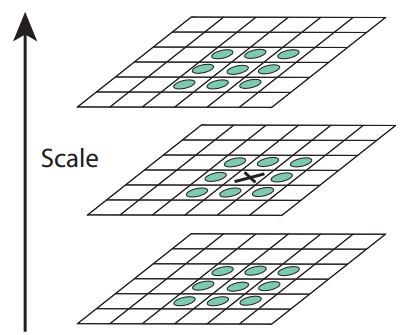
\includegraphics[scale=0.5]{pict/02/sift/sift_dgl_extremum.png}
\caption{Porównywanie otoczenia piksela w celu znalezienia lokalnego ekstremum}
\label{fig:sift_dgl_extremum}
\end{figure}
\subsubsection{Subpikselowa lokalizacja punktów charakterystycznych}
W związku, z tym, ekstrema często wypadają między sąsiadującymi pikselami, dokładną pozycję ekstremum uzyskuje się korzystając z rozwinięcia Taylora.
\begin{equation}
D(x) = D + \frac{\partial D^T}{\partial x}x + \frac{1}{2}x^T\frac{\partial^2D}{\partial x^2}x
\end{equation}

\begin{equation}
\widehat{x} = -\frac{\partial^2D}{\partial x^2}^{-1} \frac{\partial D}{\partial x}
\end{equation}



\begin{figure}[!htb]
\centering
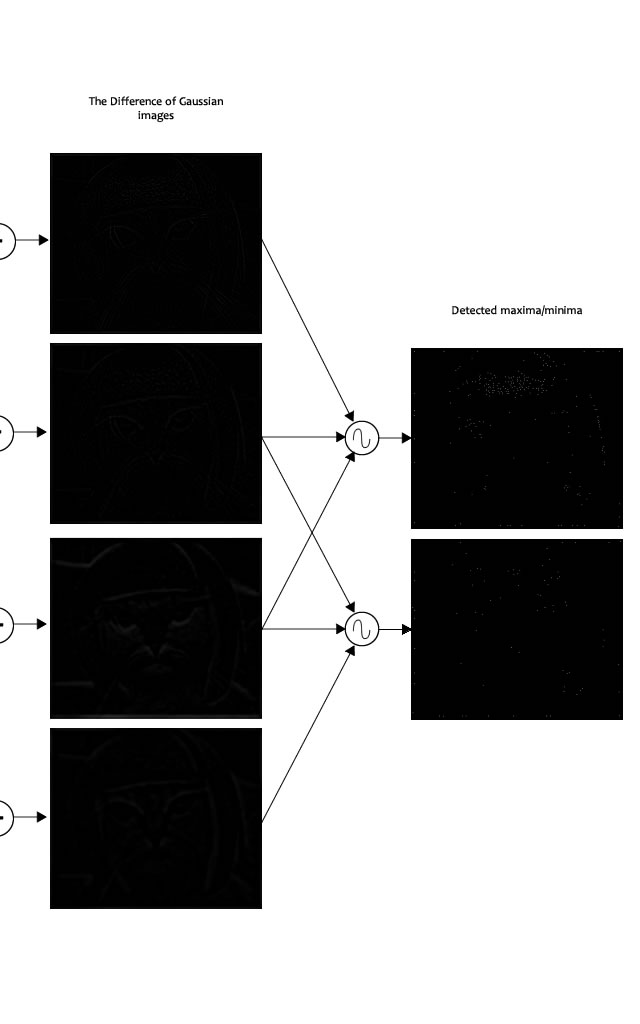
\includegraphics[width=0.8\textwidth]{pict/02/sift/sift_ais_extremum.jpg}
\caption{Przykład wyszukiwania ekstremów w obrazach różnicowych}
\label{fig:sift_ais_extremum}
\end{figure}




\subsection{Selekcja punktów charakterystycznych}
W wyniku działania wcześniej opisanych kroków algorytm generuję ogromną liczbę punktów charakterystycznych. Niestety znaczna część punktów jest słabej jakości, zbyt mało kontrastowa lub leży na krawędziach. Nie pozwala to na ich praktyczne wykorzystanie i takich punktów należy się pozbyć.
\subsubsection{Usuwanie cech mało kontrastowych}
Usuwanie cech mało kontrastowych odbywa się poprzez progowanie. Jeżeli wartość bezwzględna piksela obrazu DoG jest mniejsza niż heurystycznie dobrany próg piksel taki jest odrzucany. W pracy \cite{DGL04} autor algorytmu zakładał próg rzędu 3 \%. W przypadku gdy punktem charakterystycznym jest subpiksel, jego wartość podobnie jak pozycje wyliczamy z szeregu Taylora.
\begin{equation}
D(\widehat{x}) = D +   \frac{1}{2}\frac{\partial D}{\partial x}\widehat{x}
\end{equation}
\subsubsection{Usuwanie punktów lezących na krawędziach}
Różnica Gaussianów generuje silną odpowiedź na krawędziach. Powoduje to pewnego rodzaju przekłamania, jak np lokalizowanie punktów charakterystycznych w miejscach gdzie są one słabo określone i bardzo podatne na zakłócenia. 
W przypadku krawędzi, gradient prostopadły do niej jest duży, a równoległy mały. Warunki te nie są wystarczające do ulokowania stabilnego punktu charakterystycznego. Najlepsze punkty charakterystyczne znajdują się w rogach, ze względu na duże wartości gradientów w obu kierunkach.
W selekcji punktów charakterystycznych wykorzystuje się dwuwymiarową macierz Hesjanu \textbf{H}, która jest liczona w potencjalnym punkcie charakterystycznym i w skali jemu odpowiadającej.

\begin{equation}
\textbf{H} = 
\left[\begin{array}{cc}
D_{xx}&D_{xy}\\
D_{xy}&D_{yy}
\end{array}\right]
\end{equation}
Pochodne $D_{xx}$,$D_{yy}$,$D_{xy}$ są liczone poprzez odejmowanie pikseli z sąsiedztwa badanego punktu.


Wartości własne macierzy są proporcjonalne do głównej krzywizny obrazu różnicowego D. Na podstawie podejścia zaproponowanego przez Harrisa i Stephensona w 1988 roku \cite{HIS88}, obliczanie wartości własnych macierzy możemy zastąpić poprzez obliczenie ich stosunku. 

Niech $\alpha$ i $\beta$ będą wartościami własnymi macierzy. Ich sumę i iloczyn możemy obliczyć ze śladu i wyznacznika macierzy Hesjanu. 

\begin{equation}
Tr(\textbf{H}) = D_{xx} + D_{yy} = \alpha + \beta
\end{equation}

\begin{equation}
Det(\textbf{H}) = D_{xx} D_{yy} - {D_{xy}}^2 = \alpha  \beta
\end{equation}

Gdy wyznacznik macierzy \textbf{H} jest ujemny badany punkt jest odrzucany. W sytuacji gdy wyznacznik jest dodatni stosujemy podstawienie $\alpha = r \beta$ co pozwala nam zapisać stosunek między śladem i wyznacznikiem macierzy za pomocą samego współczynnika $r$
\begin{equation}
\frac{Tr(\textbf{H})^2}{Det(\textbf{H})} = \frac{(\alpha+\beta)^2}{\alpha\beta} = \frac{(r\beta+\beta)^2}{r\beta^2} = \frac{(r+1)^2}{r} 
\end{equation}
Aby wyeliminować odpowiedź krawędziową należy porównać stosunek głównych krzywizn badanego punktu i dokonać prostego progowania z użyciem współczynnika $r$.
 

\begin{equation}
\frac{Tr(\textbf{H})^2}{Det(\textbf{H})} < \frac{(r+1)^2}{r} 
\label{eqn:ratio_prog}
\end{equation}
Przedstawiona metoda jest bardzo efektywna obliczeniowo. Do przetestowania pojedynczego potencjalnego punktu charakterystycznego potrzebuje mniej niż 20 operacji zmiennoprzecinkowych. W badaniach \cite{DGL04} sugerowany współczynnik $r$ wynosi 10.


\subsection{Określenie orientacji punktów charakterystycznych}
Wyselekcjonowanego zbioru  punktów charakterystycznych należy przypisać orientacje. Zadanie to jest kluczowe w działaniu algorytmu, gdyż pozwala uniezależnić punkty charakterystyczne od rotacji obrazu. Na podstawie obrazu poddanemu rozmyciu Gaussa w skali rozmycia w jakiej dany punkt charakterystyczny został znaleziony wylicza się wartości i orientacje gradientów w otoczeniu punktu charakterystycznego:
\begin{equation}
m(x,y) = \sqrt{(L(x+1,y)-L(x-1,y))^2+(L(x,y+1)-L(x,y-1))^2}
\end{equation}
\begin{equation}
\theta(x,y) = atan(\frac{L(x,y+1)-L(x,y-1)}{L(x+1,y)-L(x-1,y)})
\end{equation}
\begin{figure}[!htb]
\centering
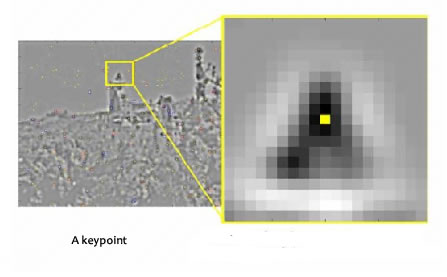
\includegraphics[width=0.8\textwidth]{pict/02/sift/sift_ais_orientation_1.jpg}
\caption{Badanie otoczenia punktu charakterystycznego - rozmycie}
\label{fig:sift_ais_orientation_1}
\end{figure}
\begin{figure}[!htb]
\centering
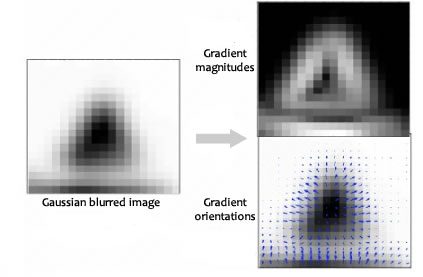
\includegraphics[width=0.8\textwidth]{pict/02/sift/sift_ais_orientation_2.jpg}
\caption{Badanie otoczenia punktu charakterystycznego - badanie gradientów}
\label{fig:sift_ais_orientation_2}
\end{figure}
W oparciu o rozkład gradientów wokół punktu charakterystycznego budowany jest histogram reprezentujący orientacje gradientów. Histogram ten jest podzielony 36 słupków o szerokości 10$^O$  pokrywający pełny zakres 360$^O$. Najwyższy pik wykresu odpowiada orientacji jaka zostanie przypisana punktowi charakterystycznemu. W sytuacji gdy inny słupek osiągnął wartość powyżej 80\% wartości maksymalnej, jego orientacja również zostaje odnotowana poprzez utworzenie dodatkowego bliźniaczego punktu, różniącego się orientacją. Według badań \cite{DGL04} tylko około 15\% posiada wielokierunkową orientacje, aczkolwiek jej uwzględnienie znacząco poprawia jakość dopasowań.
\begin{figure}[!htb]
\centering
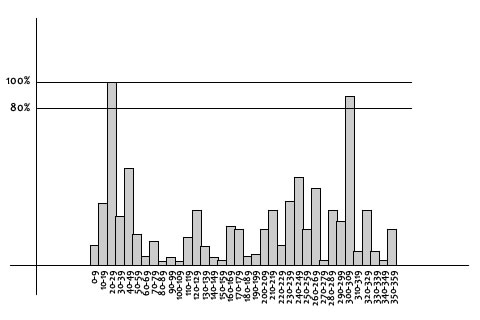
\includegraphics[width=0.8\textwidth]{pict/02/sift/sift_ais_orientation_histogram.jpg}
\caption{Histogram reprezentujący orientacje gradientów wokół punktu charakterystycznego}
\label{fig:sift_ais_orientation_histogram}
\end{figure}


\subsection{Budowa deskryptora}
Finalny etapem algorytmu SIFT jest wyliczenie  unikalnego deskryptora punktu charakterystycznego. Wokół punktu charakterystycznego badane jest okno o rozmiarze 16 na 16 pikseli podzielone na 16 sektorów. Sektor stanowi kwadrat o boku 4 pikseli. 
\begin{figure}[!htb]
\centering
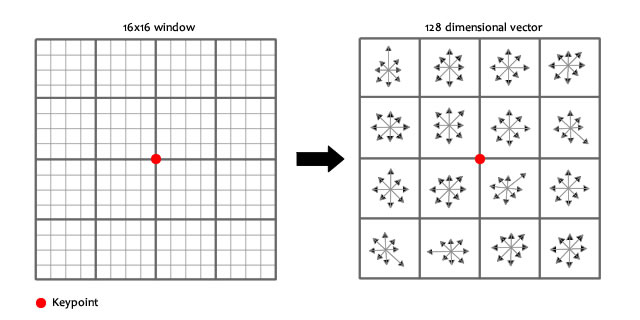
\includegraphics[width=0.8\textwidth]{pict/02/sift/sift_ais_16_16_128.jpg}
\caption{Tworzenie deskryptora punktu charakterystycznego - lokalna siatka histogramów}
\label{fig:sift_ais_16_16_128}
\end{figure}
Dla każdego pojedynczego sektora obliczane są wielkości i kierunki gradientów, które zostają zapisane za pomocą 8 wartościowego histogramu. Orientacje gradientów wyrażane są jako wielokrotności kąta 45$^O$.




\begin{figure}[!htb]
\centering
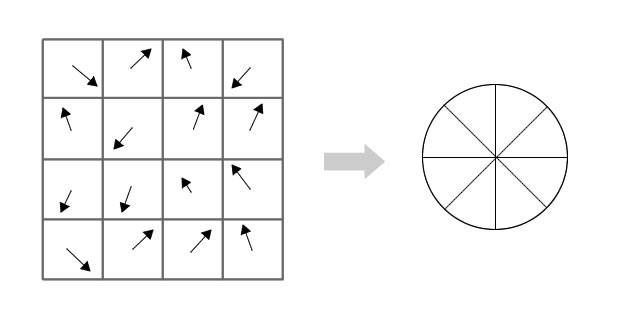
\includegraphics[width=0.8\textwidth]{pict/02/sift/sift_ais_4_4_8.jpg}
\caption{Tworzenie deskryptora punktu charakterystycznego - lokalna siatka histogramów}
\label{fig:sift_ais_4_4_8}
\end{figure}

Po obliczeniu 16 histogramów, cała tablica sektorów zostaje przeskalowana. Spowodowane to jest tym, że okna leżące bliżej punktu charakterystycznego są istotniejsze i należy im przypisać większa wagę. Analogicznie zmniejszany jest wpływ wartości znajdujących się brzegach badanego obszaru.

\begin{figure}[!htb]
\centering
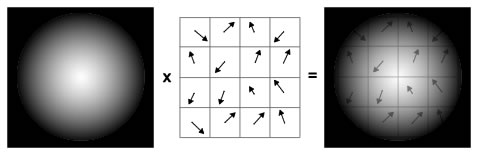
\includegraphics[width=0.8\textwidth]{pict/02/sift/sift_ais_des.jpg}
\caption{Siatka histogramów uwzględniająca odległość od punktu charakterystycznego}
\label{fig:sift_ais_des}
\end{figure}

W wyniku powyższych operacji otrzymujemy wektor 128 liczb (8 kierunkowe histogramy zgrupowane w 4 wierszach po 4 kolumny). Wektor ten jest poddawany normalizacji. 

Następnie aby uzyskać niezależność od rotacji, od wektora jest odejmowana orientacja punktu charakterystycznego obliczona w poprzednim etapie. Aby uzyskać niezależność od oświetlenia współczynniki znormalizowanego wektora, są poddawane półprogowaniu z parametrem 0,2. W sytuacji gdy jakiś współczynnik jest większy od zadanego progu, przypisywana mu jest wartość 0,2 po czym cały wektor poddawany jest ponownej normalizacji.

W wyniku całego procesu otrzymujemy 128 wymiarowy deskryptor punktu charakterystycznego.


%\begin{figure}[!htb]
%\centering
%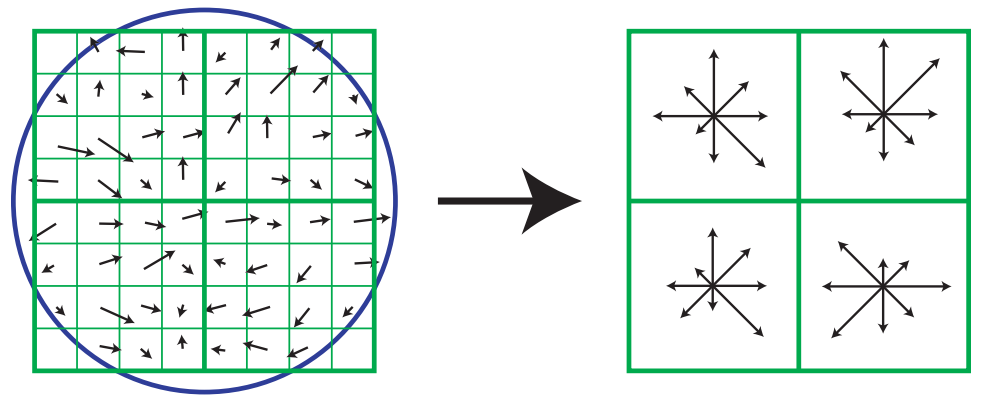
\includegraphics[width=0.8\textwidth]{pict/02/sift/sift/sift_dgl_keypoint.png}
%\caption{opis}
%\label{fig:sift_dgl_keypoint}
%\end{figure}

\FloatBarrier
\newpage
\section{Algorytm SURF}
Algorytm SURF (\textit{skrót od Speeded Up Robust Features}) został po raz pierwszy zaprezentowany w 2006 roku w pracy doktorskiej Herberta Baya \cite{HB06}. Pełny jego opis można znaleźć również w pracy\cite{HB08}. Wykorzystywany jest on w zadaniach rozpoznawania obrazów oraz w rekonstrukcji obiektów trójwymiarowych. Algorytm częściowo jest inspirowany algorytmem SIFT i podobnie jak on aby usprawnić obliczenia korzysta z aproksymacji skomplikowanych operatorów. 

Pomijając sekcję poświęconą szybkiemu rozpoznawaniu obrazów w jego działanie możemy podzielić na następujące etapy:
\begin{enumerate}
\item{obliczenie obrazów całkowych}
\item{lokalizowanie punktów charakterystycznych}
\item{konstruowanie 64 wymiarowego deskryptora punktu charakterystycznego}
\end{enumerate}
SURF podobnie jak algorytm SIFT jest chroniony patentem amerykańskim.
\subsection{Obliczenie obrazów całkowych}
Działanie algorytmu SURF rozpoczyna się od przygotowania obrazów całkowych. Są one wyliczane wg. wzoru \ref{eqn:surf_integral_images}.
\begin{equation}
I_{\sum}(x,y) = \sum\limits_{x'=0}^{ x} \sum\limits_{y'=0}^{y} I(x',y')
\label{eqn:surf_integral_images}
\end{equation}
Przygotowanie reprezentacji badanego obrazu w postaci całkowej pozwala, zredukować obliczenia intensywności dowolnego fragmentu obrazu do trzech prostych operacji arytmetycznych o stałym czasie wykonania. Ma to kluczowe znaczenie w przypadku analizy dużych fragmentów obrazów.


\begin{figure}[!htb]
\centering
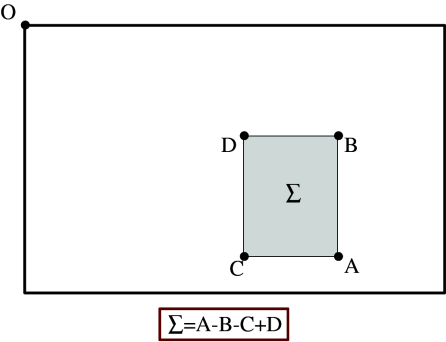
\includegraphics[width=0.8\textwidth]{pict/02/surf/surf_bay_integral_image.png}
\caption{Obliczanie intensywności wybranego obszaru w oparciu o obrazy całkowe}
\label{fig:surf_bay_integral_image}
\end{figure}



\subsection{Lokalizowanie punktów charakterystycznych}
\subsubsection{Wykrywanie punktów charakterystycznych za pomocą macierzy Hesjanu}
Algorytm do wykrywania obszarów charakterystycznych wykorzystuje macierz Hesjanu. Obszary te są lokowane w miejscach, w których wyznacznik macierzy osiąga lokalne maksimum.
\begin{equation}
\textbf{H}(x,y,\sigma) = 
\left[\begin{array}{cc}
L_{xx}(x,y,\sigma)&L_{xy}(x,y,\sigma)\\
L_{xy}(x,y,\sigma)&L_{yy}(y,y,\sigma)
\end{array}\right]
\end{equation}
Wyrażenie $L_{xx}(x,y,\sigma)$ to obraz splotu pochodnej cząstkowej drugiego stopnia funkcji rozmycia Gaussa ($D_{xx}=\frac{\partial^2}{\partial x^2}\frac{1}{2\pi\sigma^2}e^{-\frac{x^2+y^2}{2\sigma^2}}$) i obrazu I w punkcie (x,y). Analogicznie $L_{yy}(x,y,\sigma)$ i $L_{xz}(x,y,\sigma)$. Przedstawia je rysunek \ref{pict:surf_exact_kernel}

\begin{figure}
\centering
\subfigure[$D_{xx}$]{

\includegraphics[scale=0.5]{pict/02/surf/dxx.png}}
\subfigure[$D_{yy}$]{

\includegraphics[scale=0.5]{pict/02/surf/dyy.png}}
\subfigure[$D_{xy}$]{

\includegraphics[scale=0.5]{pict/02/surf/dxy.png}}
\caption{Pochodne cząstkowe drugiego stopnia funkcji rozmycia Gaussa}
\label{pict:surf_exact_kernel}
\end{figure}
W praktyce stosuję się powyższe jądra w dyskretnej formie co przedstawia rysunek \ref{fig:surf_bay_gaussian_discretization}. Skutkuje to pogorszeniem jakości pracy operatorów w sytuacji gdy obraz jest obrócony o nieparzystą wieloktrotność kąta $45^O$ i może prowadzić do pojawienia się artefaktów. 

\begin{figure}[!htb]
\centering
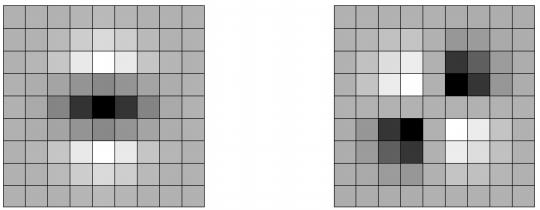
\includegraphics[width=0.8\textwidth]{pict/02/surf/surf_bay_gaussian_discretization.png}
\caption{Dyskretne pochodne cząstkowe drugiego stopnia Gaussianów}
\label{fig:surf_bay_gaussian_discretization}
\end{figure}
\subsubsection{Aproksymacja jąder rozmycia}
Bay podobnie jak Lowe w algorytmie SIFT zastosował podejście polegające na dużym uproszeniu realizowanych operacji. Jądra rozmycia zostały w radykalny sposób aproksymowane [rysunek \ref{fig:surf_bay_gaussian_approximation}].

\begin{figure}[!htb]
\centering
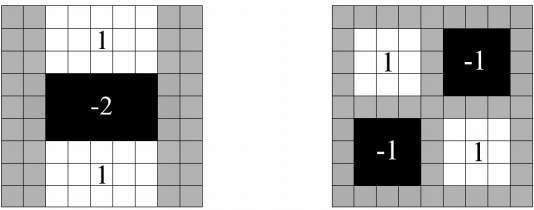
\includegraphics[width=0.8\textwidth]{pict/02/surf/surf_bay_gaussian_approximation.png}
\caption{Aproksymacje pochodnych cząstkowych drugiego stopnia Gaussianów}
\label{fig:surf_bay_gaussian_approximation}
\end{figure}

W związku z zastosowaniem aproksymowanych okien rozmycia wyrażenie na wyznacznik Hesjanu przyjmuje następująca postać:
\begin{equation}
det(\textbf{H}^{(a)}) = L_{xx}^{(a)} L_{yy}^{(a)}-(\omega L_{xy}^{(a)})^2)
\label{eqn:det_aprox}
\end{equation}
Gdzie $L_{xx}^{(a)}$, $L_{yy}^{(a)}$, $L_{xy}^{(a)}$ to sploty obrazu I z aproksymowanymi oknami rozmycia, a współczynnik $\omega$ to waga potrzebna zachowania energii jąder Gaussowski przy korzystaniu z ich uproszczonej postaci. Obliczana jest ona według wyrażenia \ref{eqn:frobo}, gdzie $\|\|_F$ oznacza normę Frobeniusa.


\begin{equation}
\omega = \frac{\|L_{xy}(\sigma)\|_F\|D_{yy}(rozmiar-okna)\|_F}{\|L_{yy}(\sigma)\|_F\|D_{xy}(rozmiar-okna)\|_F}
\label{eqn:frobo}
\end{equation}
Dla okna rozmycia $\sigma=1.2$ o wymiarach $9\times9$ współczynnik $\omega$ wynosi:
\begin{equation}
\omega = \frac{\|L_{xy}(1.2)\|_F\|D_{yy}(9)\|_F}{\|L_{1.2}(\sigma)\|_F\|D_{xy}(9)\|_F} = 0.9127\simeq0.9
\end{equation}
Teoretycznie każdemu rozmyciu i rozmiarowi okna odpowiada inna wartość wagi $\omega$. Praktyka jednak pokazuje, że dla usprawnienia pracy algorytmu możemy $\omega$ traktować jaką stałą, bez dużej straty dokładności. 

 W sposób znaczny przyśpiesza to obliczenia, a jak wykazały badania \cite{HB06} nie tylko nie pogarsza to wyników, a wręcz je polepsza [rysunek \ref{fig:surf_bay_compare_fast}].




\begin{figure}[!htb]
\centering
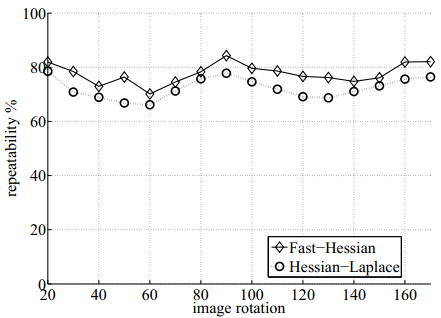
\includegraphics[scale=0.8]{pict/02/surf/surf_bay_compare_fast.png}
\caption{Porównanie działania operatorów dokładnych i aproksymowanych w zależności od kąta rotacji obrazu}
\label{fig:surf_bay_compare_fast}
\end{figure}

\subsubsection{Skalo-przestrzenna reprezantacja orbazu}
Lokalizowanie punktów kluczowych odbywa się w różnych skalach obrazu. Obrazy skalo-przestrzenne są najczęściej reprezentowane w postaci piramidy obrazów. Kolejne obrazy są poddawane progresywnemu rozmyciu oraz podpróbkowane, tworząc oktawy.
\begin{figure}[!htb]
\centering
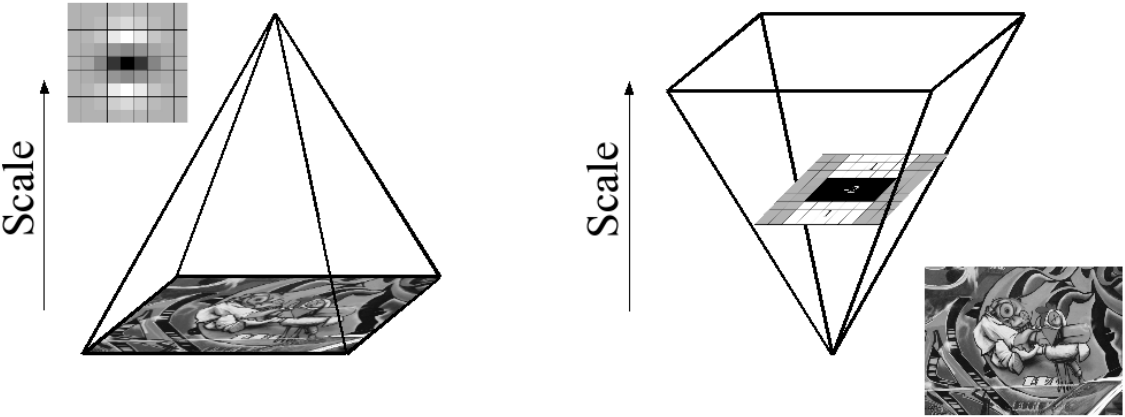
\includegraphics[width=0.8\textwidth]{pict/02/surf/surf_bay_scale_piramid.png}
\caption{Piramida skalo-przestrzenna}
\label{fig:surf_bay_scale_piramid}
\end{figure}


Dzięki zastosowaniu obrazów całkowych i błyskawicznie skalowalnych okien rozmycia, operacje skalo-przestrzenne dają się w łatwy sposób zrównoleglić.



\subsubsection{Skalowanie jąder rozmycia}
\begin{figure}[!htb]
\centering
\subfigure[$D_{yy}$]{
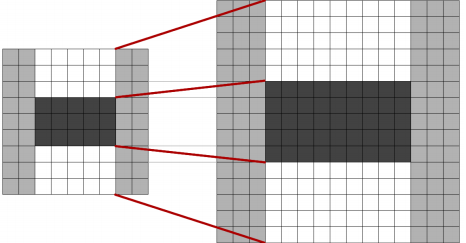
\includegraphics[scale=0.62]{pict/02/surf/surf_bay_prescale_gaussian_1.png}}
\subfigure[$D_{xy}$]{
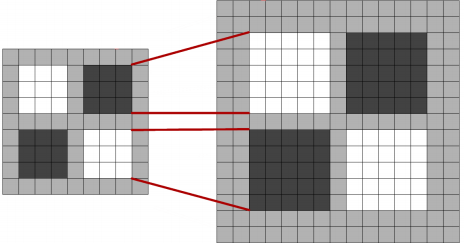
\includegraphics[scale=0.62]{pict/02/surf/surf_bay_prescale_gaussian_2.png}}
\caption{Przeskalowane okna rozmycia}
\label{fig:surf_bay_prescale_gaussian}
\end{figure}
Każde okno rozmycia jest kwadratem o boku $3l$ które można opisać za pomocą następujących wyrażeń:

\begin{align}
 l &= 2^oi+1\\
\label{eqn:liczym_l}
\end{align}
gdzie:

{\centering
\begin{tabular}{cclll}
o & - &  numer oktawy     &&$o=1,2,3,4,...$\\ 
i & - & stopień rozmycia w oktawie &&$i=1,2,3,4$\\ 
\end{tabular} 
}
W związku z powyższym wzór na odchylenie standardowe rozmycia Gaussa $\sigma$ możemy zapisać:

\begin{align}
\sigma &= \frac{1.2}{3}l\\
\label{eqn:sigma_o_i_l}
\end{align}


\begin{equation}
D_{xx} = \left\lbrace \begin{array}{ccl}
-2&&  (x,y) \in [-\frac{l}{2},\frac{l}{2}]\times]-l,l[\\
+1&&  (x,y) \in [-\frac{l}{2},\frac{l}{2}]\times]-l,l[\times[-\frac{3l}{2},\frac{3l}{2}]\setminus]-l,l[ \\
0 && reszta
\end{array} \right.
\end{equation}

\begin{equation}
D_{yy} = \left\lbrace \begin{array}{ccl}
-2&&  (x,y) \in ]-l,l[\times[-\frac{l}{2},\frac{l}{2}]\\
+1&&  (x,y) \in ]-l,l[\times[-\frac{3l}{2},\frac{3l}{2}]\setminus]-l,l[\times[-\frac{l}{2},\frac{l}{2}] \\
0 && reszta 
\end{array} \right.
\end{equation}

\begin{equation}
D_{xy} = \left\lbrace \begin{array}{ccl}
+1&&  (x,y) \in ]0,-l]\times]0,+l]\bigcap]0,+l]\times[-l,0[ \\
-1&&  (x,y) \in [-l,0[\times[-l,0[\bigcap]0,+l]\times]0,+l]\\
0 && reszta
\end{array} \right.
\end{equation}




\begin{equation}
\sigma^2=\frac{L^2-1}{12}
\label{eqn:sigma_2_L}
\end{equation}


 

\begin{figure}[!htb]
\centering
\subfigure[$D_{yy}$]{
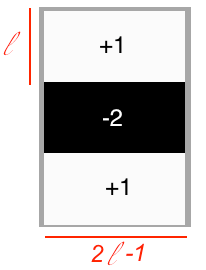
\includegraphics[scale=1]{pict/02/surf/dyy_prescale.png}}
\subfigure[$D_{xy}$]{
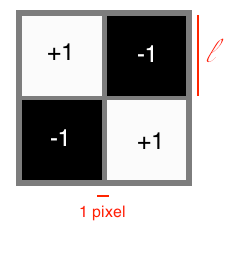
\includegraphics[scale=1]{pict/02/surf/dxy_prescale.png}}
\caption{Okna rozmycia}
\label{fig:surf_bay_prescale_gaussian_3}
\end{figure}

\begin{table}
\centering

\begin{tabular}{|c|c|c|c|c|c|c|}
  \hline 
   o & i & $\sigma$ & l & L & $\lambda$ & $\omega$ \\ 
  \hline 
   1 & 1 & 1,2 & 3 & 4,275 & 2 & 0,9127 \\ 
  \hline 
     & 2 & 2,0 & 5 & 7,000 & 4 & 0,9487 \\ 
  \hline 
     & 3 & 2,8 & 7 & 9,751 & 6 & 0,9636 \\ 
  \hline 
     & 4 & 3,6 & 9 & 12,511 & 7 & 0,9718 \\ 
  \hline 
   2 & 1 & 2,0 &5 & 8,000 & 4 & 0,9487 \\ 
  \hline 
     & 2 & 3,6 & 9 & 12,510 & 7 & 0,9718 \\ 
  \hline 
     & 3 & 5,2 & 13 & 18,041 & 10 & 0,9806 \\ 
  \hline 
     & 4 & 6,8 &17 & 23,577 & 14 & 0,9852 \\ 
  \hline 
   3 & 1 & 3,6 & 9 & 12,510 & 7 & 0,9718 \\ 
  \hline 
     & 2 & 6,8 & 17 & 23,577 & 14 & 0,9852 \\ 
  \hline 
     & 3 & 10,0 & 25 & 34,655 & 20 & 0,9900 \\ 
  \hline 
    & 4 &13,2 & 33 & 45,737 & 26 & 0,9924 \\ 
  \hline 
   4 & 1& 6,8 & 17 & 23,577 & 14 & 0,9852 \\ 
  \hline 
    & 2 &13,2 & 33 & 45,737 & 26 & 0,9924 \\ 
  \hline 
    & 3 &19,6 & 49 & 67,903 & 39 & 0,9949 \\ 
  \hline 
    & 4 &26,0 & 65 & 90,072 & 52 & 0,9962 \\ 
  \hline 
  \end{tabular}
  \caption{Wartości charakterystyczne dla okien aproksymowanych filtrów rozmycia}
  \label{tab:surf_parameters}
\end{table}

\begin{figure}[!htb]
\centering
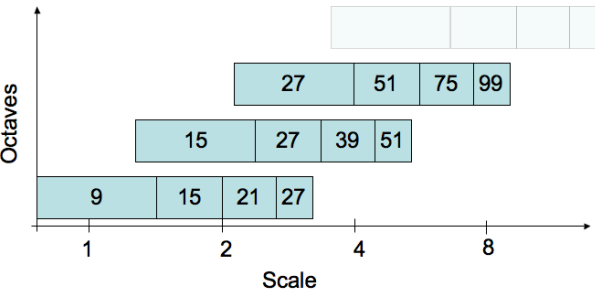
\includegraphics[width=0.8\textwidth]{pict/02/surf/surf_bay_octave_scale.png}
\caption{Rozmiar okna filtru w zależności od oktawy i stopnia rozmycia}
\label{fig:surf_bay_octave_scale}
\end{figure}
Tabela \ref{tab:surf_parameters} przedstawia charakterystyczne parametry filtrów. Zostały w niej przedstawione właściwości dla 4 pierwszych oktaw. Algorytm zakłada możliwość analizowania większej ilości oktaw. Ich parametry są obliczane w analogiczny sposób, dopóki okno filtru nie przekracza rozmiaru obrazu. W praktyce jednak badania najczęściej ogranicza się do 4 pierwszych oktaw, gdyż ze wzrostem skali znacząco spada liczba lokalizowanych punktów charakterystycznych [wykres \ref{fig:surf_bay_scale_histogram}].


\begin{figure}[!htb]
\centering
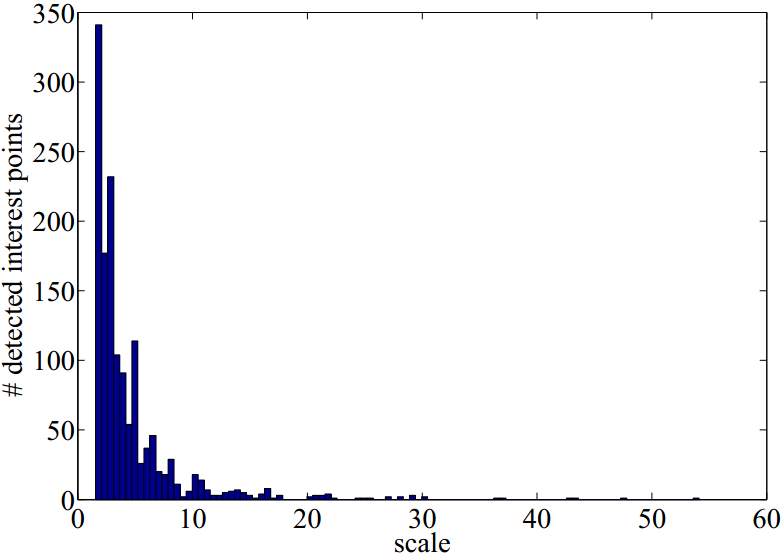
\includegraphics[scale=0.7]{pict/02/surf/surf_bay_scale_histogram.png}
\caption{Ilość lokalizowanych punktów charakterystycznych w zależności od skali}
\label{fig:surf_bay_scale_histogram}
\end{figure}










\subsection{Określenie orientacji punktów charakterystycznych}
Do określenia orientacji punktu charakterystycznego wykorzystywana jest falka Haara. Dla pikseli znajdujących się w otoczeniu punktu charakterystycznego liczone są odpowiedzi falki Haara w kierunku poziomym i pionowym. Poprzez otoczenie rozumiany jest kołowy obszar o promieniu $6\sigma$, gdzie $\sigma$ odpowiada skali w jakiej został zlokalizowany punkt. Podobnie rozmiar falki zależy od skali. Do jej liczenia wykorzystujemy okno o boku $4\sigma$. Dzięki zastosowaniu przygotowanych wcześniej obrazów całkowych liczba operacji potrzebnych do policzenia odpowiedzi w jednym kierunku została zredukowana do 6.


Odpowiedzi falek są reprezentowane na układzie współrzędnych. Oś OX reprezentuje odpowiedzi poziome, OY pionowe, a punkt przecięcia stanowi punkt charakterystyczny. Następnie wykorzystując obracające się wokół początku układu współrzędnych okno będące wycinkiem koła o kącie $\frac{\pi}{3}$. Odpowiedzi znajdujące się wewnątrz okna są sumowane. Suma odpowiedzi stanowi długość wektora związanego z kątem w jakim znajduje się okno. Kąt orientacji punktu charakterystycznego jest kątem w którym długość wektora sum odpowiedzi jest największa [rys.\ref{fig:surf_bay_orientation_assignment_c}].

\begin{figure}[!htb]
\centering
\subfigure[]{
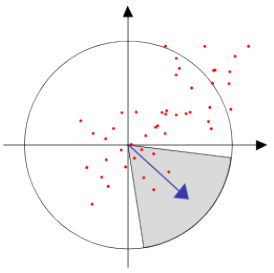
\includegraphics[scale=0.6]{pict/02/surf/surf_bay_orientation_assignment_1.png}}
\subfigure[]{
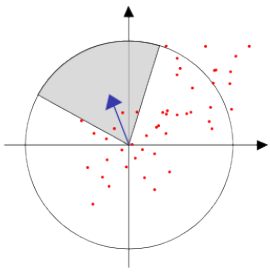
\includegraphics[scale=0.6]{pict/02/surf/surf_bay_orientation_assignment_2.png}}
\subfigure[]{
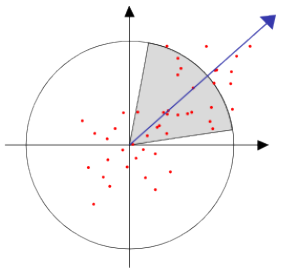
\includegraphics[scale=0.6]{pict/02/surf/surf_bay_orientation_assignment_3.png}
\label{fig:surf_bay_orientation_assignment_c}}

\caption{Badanie orientacji punktu charakterystycznego}
\label{fig:surf_bay_orientation_assignment}
\end{figure}


\subsection{Budowa deskryptora}
Podobnie jak algorytm SIFT, SURF do budowy deskryptora wykorzystuje informacje o otoczeniu punktu charakterystycznego. Wokół badanego punktu analizowany jest kwadratowy obszar o boku $20\sigma$. 

Okno to jest zorientowanie zgodnie z kierunkiem wyznaczonym w poprzednim kroku i podzielone na 16 regularnych subregionów. Każdy subregion jest w równych odstępach próbkowany w efekcie czego otrzymujemy zbiór $5\times5$ pikseli. Dla wycinka reprezentującego subregion liczona jest falka Haara w kierunku równoległym i normalnym do orientacji punktu charakterystycznego.  Falka ta ma rozmiar $2\sigma$ W praktyce aby zwiększyć szybkość działania algorytmu falki są liczone dla nie obróconego obrazu, a następnie ich odpowiedzi są interpolowane do kierunku rotacji. 
\begin{figure}[!htb]
\centering
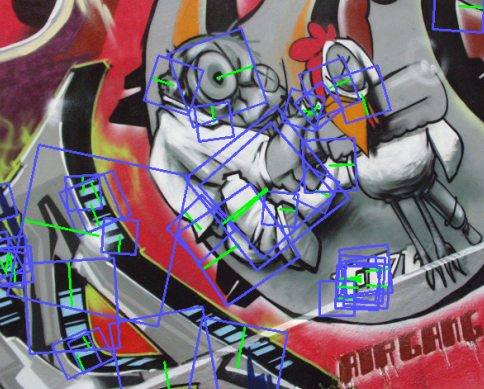
\includegraphics[scale=0.8]{pict/02/surf/surf_bay_example.png}
\caption{Badane obszary charakterystyczne}
\label{fig:surf_bay_example}
\end{figure}
W celu minimalizacji błędów spowodowanych geometrycznymi deformacjami odpowiedzi falek $d_x$ i $d_y$ są normalizowane rozkładem Gaussa z rozkładem równym $3.3\sigma$ (\textit{gdzie $\sigma$ oznacza skale w jakiej badany jest obszar}).

\begin{figure}[!htb]
\centering
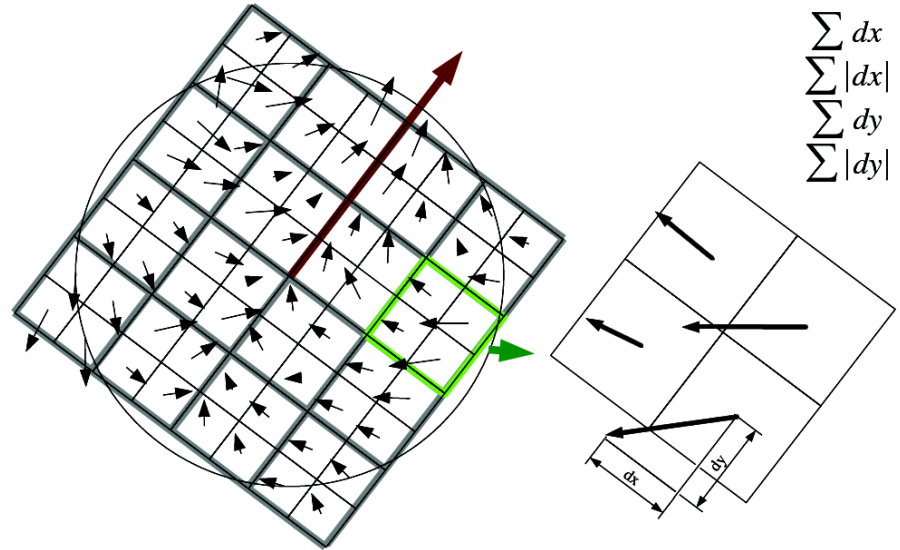
\includegraphics[width=0.8\textwidth]{pict/02/surf/surf_bay_scale_descriptor.png}
\caption{Badanie otoczenia punktu charakterystycznego}
\label{fig:surf_bay_scale_descriptor}
\end{figure}

Falki w obrębie jednego subregionu są sumowane. Ponadto sumowaniu poddawne są wartości bezwzględne falek. Zabieg ten ma na celu pozyskanie informacji o biegunowości instensywności zmian. W wyniku tych działań otrzymujemy 4 wymiarowy wektor opisujący subregion.

\begin{equation}
v_{subregion} = \left[ \sum d_x,\sum d_y,\sum |d_x|,\sum |d_y|\right] 
\end{equation}

\begin{figure}[!htb]
\centering
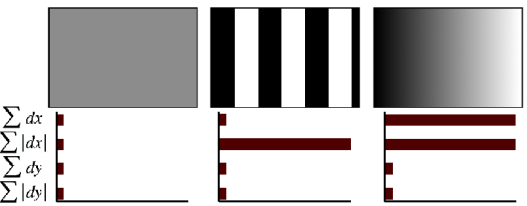
\includegraphics[width=0.8\textwidth]{pict/02/surf/surf_bay_gradient.png}
\caption{Przykłady wektorów opisujących subregiony w zależności od natury obszaru charakterystycznego}
\label{fig:surf_bay_gradient}
\end{figure}

W skład deskryptora punktu charakterystycznego wchodzi 16 subregionów w efekcie czego otrzymujemy 64 wymiarowy wektor punktu charakterystycznego. Algorytmu posiada wariacje różniące się rozdzielczością na jaką jest podzielony badany obszar charakterystyczny. Badania \cite{HB08} wykazują jednak 64 wymiarowy deskryptor jest rozwiązaniem najlepszym i optymalnym [\ref{fig:surf_bay_compare}]. W sytuacji, w której lekki spadek jakości jest akceptowalny na rzecz znaczącej poprawy czasu dopasowywania punktów charakterystycznych, wartym rozważenia jest deskryptor SURF-36 (\textit{$3\times3\times4$})
\begin{figure}[!htb]
\centering
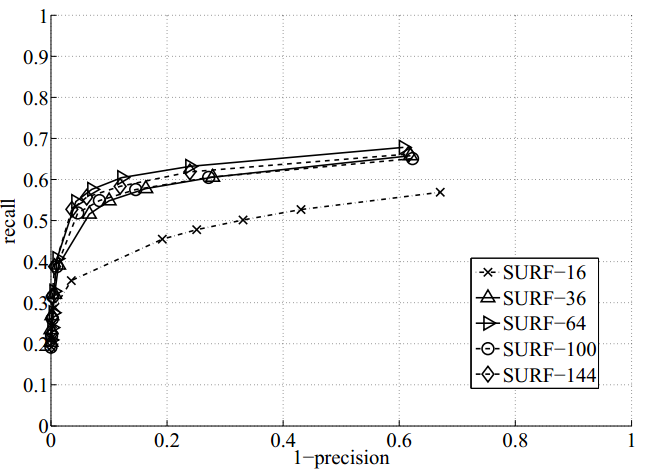
\includegraphics[width=0.8\textwidth]{pict/02/surf/surf_bay_compare_dim.png}
\caption{Porównanie deskryptorów SURF}
\label{fig:surf_bay_compare}
\end{figure}


Otrzymany deskryptor dzięki zastosowaniu falek jest niezależny od rotacji,skali, zmiennego  oświetlenia. Po normalizacji do wektora jednostkowego uzyskuje ponadto niezależność od kontrastu. Co więcej dzięki zastosowaniu całkowania informacji gradientach w subregionach, algorytm SURF jest również bardziej odporny na zaszumienie obrazu niż algorytm SIFT [rys. \ref{fig:surf_bay_clean_noisy}]. 
\begin{figure}[!htb]
\centering
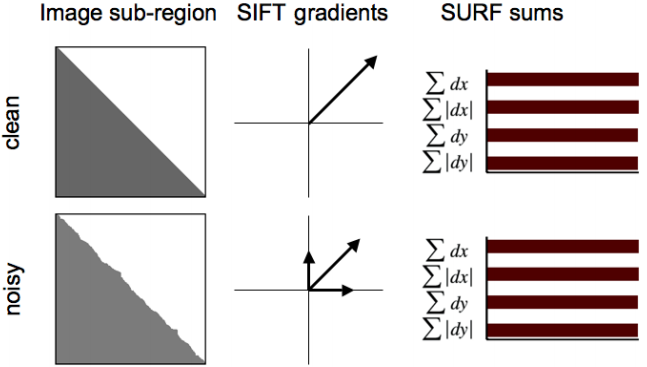
\includegraphics[width=0.8\textwidth]{pict/02/surf/surf_bay_clean_noisy.png}
\caption{Wpływ szumu na wygląd deskryptorów subregionów algorytmów SIFT i SURF}
\label{fig:surf_bay_clean_noisy}
\end{figure}
\FloatBarrier
\newpage
\section{Algorytm STAR}
Algorytm STAR to zoptymalizowany algorytm {CenSurE} (\textit{skr. Center Surround Extremas}) \cite{CENS} rozwijany w laboratorium robotyki Willow Garrage. Stanowi rozwinięcie podejścia zastosowanego w  algorytmie SURF. 


\subsection{Obliczenie pochyłych obrazów całkowych}

Algorytm STAR podobnie jak SURF korzysta z obrazów całkowych. Raz obliczona reprezentacja obrazu może być wielokrotnie wykorzystywana w trakcie analizy. W sposób znaczący przyśpiesza to prace algorytmu i zapewnia stały czas wykonywania operacji niezależnie od rozmiaru badanego obszaru. Ze względu na użycie w algorytmie STAR filtrów o skomplikowanych kształtach modyfikacji uległa funkcja obliczająca obrazy. Zamiast stosowanego w SURF wzoru:
\begin{equation}
I_{\sum}(x,y) = \sum\limits_{x'=0}^{ x} \sum\limits_{y'=0}^{y} I(x',y')
\label{eqn:star_integral_images_old}
\end{equation}
obrazy całkowe w algorytmie STAR obliczane są według następującej formuły:
\begin{equation}
I_{\sum\alpha}(x,y) = \sum\limits_{y'=0}^{ y} \sum\limits_{x'=0}^{x+\alpha(y-y')} I(x',y')
\label{eqn:star_integral_images}
\end{equation}
gdzie $\alpha$ jest stałą zależną od rodzaju stosowanego filtru. Gdy $\alpha=0$ wzór \ref{eqn:star_integral_images} przyjmuje postać wzoru \ref{eqn:star_integral_images_old}. Gdy $\alpha>0$ obszar obrazu całkowego jest pochylony w prawo (\textit{jak na rysunku \ref{fig:cs_trapezoidal}}), a gdy $\alpha<0$ w lewo. 

\begin{figure}
\centering
\subfigure[]{
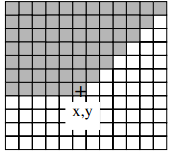
\includegraphics[scale=0.8]{pict/02/star/cs_integral_image_a.png}}
\subfigure[]{
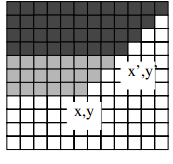
\includegraphics[scale=0.8]{pict/02/star/cs_integral_image_b.png}}
\caption{Przykład zastosowania pochyłych obrazów całkowych dla trapezoidalnego obszaru}
\label{fig:cs_trapezoidal}
\end{figure}







\subsection{Lokalizowanie punktów charakterystycznych}


Do lokalizowania punktów charakterystycznych algorytm STAR wykorzystuje dwustopniowe filtry otoczeniowo-centryczne, stanowiące łatwą i szybką w obliczeniach aproksymacje Laplasjanu. W STAR zastosowano inspirowany falkami Haara dwustopniowy filtr otoczeniowo-centryczny[rys. \ref{fig:star_bi_filters}].



\begin{figure}[!htb]
\centering
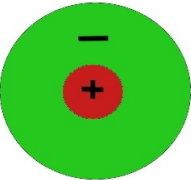
\includegraphics[scale=0.5]{pict/02/star/wg_haar.png}
\caption{Schemat dwustopniowego filtru otoczeniowo-centrycznego}
\label{fig:wg_haar}
\end{figure}

\subsubsection{Dwustopniowe filtry otoczeniowo-centryczne}

W ramach prac nad algorytmem {CenSurE} przetestowano szereg dwustopniowych filtrów począwszy od kołowego operatora LoG po dwustopniowy filtr kwadratowy. Filtr kołowy jest najwierniejszą reprezentacją Laplasjanu, aczkolwiek jest najbardziej złożony obliczeniowo. Bardzo szybkie filtry kwadratowe są z kolei podatne na rotacje obrazu i ich efektywność spada przy obrotach o nieparzyste wielokrotności kąta $45^O$. Odpowiedni filtr powinien być kompromisem między liczbą stopni symetrii i złożonością obliczeniową. W algorytmie {CenSurE} zastosowano filtr ośmiokątny [rys. \ref{fig:cs_okt}] dający się łatwo obliczać dzięki zastosowaniu pochyłych obrazów całkowych. Optymalizując algorytm {CenSurE} wypracowano rozwiązanie złożone 2 obróconych względem siebie o kąt $45^O$ kwadratów [rys. \ref{fig:wg_circle_aprox}] tworzących gwiazdę - skąd nazwa algorytm STAR (\textit{w tłumaczeniu z angielskiego "gwiazda"}).



\begin{figure}[!htb]
\centering
\subfigure[]{

\includegraphics[height=25mm]{pict/02/star/cs_circle_aprox_a.png}
}
\subfigure[]{
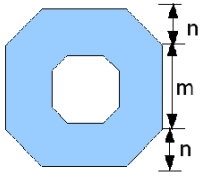
\includegraphics[height=25mm]{pict/02/star/cs_circle_aprox_b.png}
\label{fig:cs_okt}
}
\subfigure[]{

\includegraphics[height=25mm]{pict/02/star/cs_circle_aprox_c.png}
}
\subfigure[]{
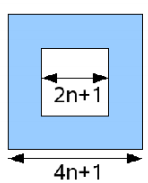
\includegraphics[height=25mm]{pict/02/star/cs_circle_aprox_d.png}
}
\caption{Dwustopniowe filtry otoczeniowo-centryczne}
\label{fig:star_bi_filters}
\end{figure}


\begin{figure}
\centering
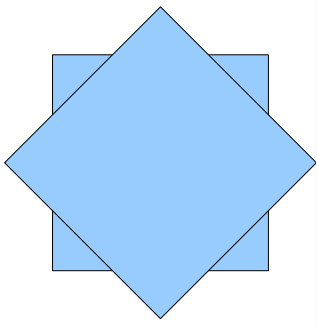
\includegraphics[height=35mm]{pict/02/star/wg_circle_aprox.png}
\caption{Dwustopniowy filtr otoczeniowo-centryczny wykorzystywany w algorytmie STAR}
\label{fig:wg_circle_aprox}
\end{figure}

Zastosowanie 2 okien o jednakowej powierzchni wyeliminowało problem równoważenia odpowiedzi dodatnich i ujemnych, oraz znacznie uprościło obliczenia. Podobnie jak w algorytmie SURF aby zwiększyć skale w jakiej lokalizujemy punkt charakterystyczny należy zwiększyć rozmiar filtra. 

\subsubsection{Ekstrema jako potencjalne punkty charakterystyczne}

Dla pojedynczego piksela obrazu jest liczone 7 odpowiedzi falek otoczeniowo-centrycznych o różnych rozmiarach. Każda falka reprezentuje obraz w innej skali. Algorytm dopuszcza liczenie większej ilości filtrów, aczkolwiek do większości zastosowań 7 okien jest liczbą wystarczającą.

Po obliczeniu odpowiedzi lokalizowane są lokalne ekstrema. Wartości falek są porównywane w pionowym i poziomym otoczeniu podobnie jak w omówionych wcześniej algorytmach. Jako potencjalne punkty charakterystyczne wybierane są piksele, które w swoim sąsiedztwie osiągają wartości ekstremalne. 

\subsection{Selekcja punktów charakterystycznych}
\subsubsection{Eliminacja słabych punktów}
Wartość bezwzględna odpowiedzi filtru dostarcza informacji o jakości punktu charakterystycznego. Im wartość ta jest większa tym punkt jest bardziej powtarzalny. W celu poprawy stabilności lokalizowanych dokonuje się progowania i odrzuca punkty o małej wartości bezwzględnej.
\subsubsection{Usuwanie punktów lezących na krawędziach}
Jak zostało opisane przy omawianiu algorytmu SIFT aby wybrać najbardziej stabilne cechy obrazu ze zbioru punktów charakterystycznych należy usunąć punkty leżące na krawędziach.W odróżnieniu do algorytmów SIFT i SURF, w algorytmie STAR zamiast macierzy Hesjanu użyto miary Harrisa.

\begin{equation}
\textbf{H} = 
\left[\begin{array}{cc}
\sum L_{x}^2&\sum L_{x}L_{y}\\
\sum L_{x}L_{y}&\sum L_{y}^2
\end{array}\right]
\end{equation}
$L_{x}$ i $L_{y}$ są pochodnymi funkcji filtru w kierunkach x i y, a sumowanie odbywa się w obrębie okna w jakim punkt charakterystyczny został zlokalizowany.


Dalsza część postępowanie jest analogiczna jak we wspomnianym algorytmie SIFT. Badany jest wyznacznik i ślad macierzy na podstawie których określa się współczynnik głównych krzywizn. W oparciu o obliczony współczynnik piksele poddawane są progowaniu [wzór \ref{eqn:ratio_prog}]. Domyślna wartość progu wynosi 10.







\FloatBarrier
\newpage
\section{Algorytm FAST}
Algorytm FAST (\textit{skr. Features from Accelerated Segment Test})został opublikowany przez Edwarda Rostena i Toma Drummonda w 2006 roku \cite{rosten_2006_machine} \cite{rosten_2008_faster}.  Algorytm ten służy do lokalizowania rogów w obrazie, które mogą być wykorzystane do zadań rozpoznawania i śledzenia. 

W odróżnieniu do wcześniej omawianych algorytmów FAST nie dokonuje "globalnej" analizy obrazu w poszukiwaniu cech charakterystycznych. Wykorzystując algorytmy uczenia maszynowego bada małe wycinki obrazu.

FAST nie dokonuje wieloskalowego poszukiwania punktów charakterystycznych. Chcąc osiągnąć niezależność od skali z oryginalnego obrazu należy wygenerować piramidę skalową, czyli zbiór obrazów reprezentujących widoki w różnych skalach.

\subsection{Zasady egzaminowania}
Jak wspomniano we wstępie, algorytm FAST należy do grupy algorytmów badających indywidualnie segmenty obrazu. Segment stanowi punkt $p$ i utworzony wokół niego okrąg składający się z 16 pikseli [rys. \ref{fig:fast_test_segment}]. 

Punkt $p$ jest uznawany jako róg jeżeli istnieje zbiór $n$ sąsiadujących pikseli okręgu, które są jaśniejsze od  intensywności punktu $p$ powiększonej o wartość progu $t$ ($I_p + t$), lub ciemniejsze od intensywności punktu $p$ pomniejszonej o próg $t$ ($I_p - t$). 

Jako wartość $n$ najczęściej przyjmuje się liczbę 12. W praktyce badanie punktu rozpoczyna się od zbadania 4 pikseli umieszczonych w głównych osiach punktu $p$. Dla rysunku \ref{fig:fast_test_segment} są to piksele 1,5,9,13. Jeżeli punkt $p$ jest rogiem, wówczas co najmniej 3 z 4 egzaminowanych pikseli muszą być jaśniejsze niż $I_p + t$ lub ciemniejsze niż $I_p - t$. Test ten pozwala w szybki sposób wykluczyć dużą liczbę punktów. Dla pozostałych punktów, które przeszły przez wstępny proces selekcji, badane są wszystkie piksele w otaczającym je segmencie.

Przytoczona metoda cechuję się dużą wydajnością, aczkolwiek jej autorzy zwracają uwagę na następujące wady:
\begin{enumerate}
\item Aby móc skutecznie zastosować szybki test wstępny 4 pikseli $n$ musi wynosić 12.
\item Wybór i kolejność testowania 4 pikseli w szybkim teście wpływa na rozkład lokalizowania punktów. Wada ta nabiera znaczenie przy zastosowaniach w czasie rzeczywistym.
\item Informacje uzyskane w szybkim teście 4 pikseli są niewykorzystywane przy dokładnym badaniu punktu.
\item Metoda może lokalizować wiele punków stykających się ze sobą.
\end{enumerate}



\begin{figure}[!htb]
\centering
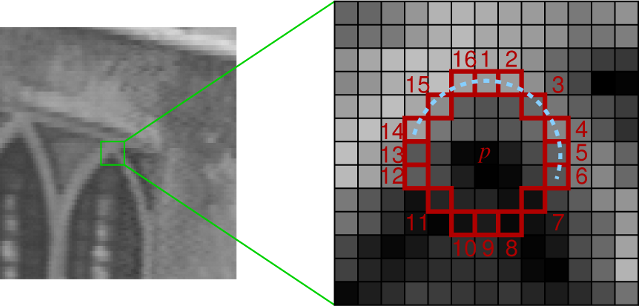
\includegraphics[width=0.8\textwidth]{pict/02/fast/fast_test_segment.png}
\caption{Badanie otoczenia punktu potencjalnego rogu}
\label{fig:fast_test_segment}
\end{figure}





\subsection{Uczenie maszynowe}
Algorytm FAST w swoim działaniu wykorzystuje metody uczenia maszynowego. Proces ten jest podzielony na dwa etapy:
\begin{enumerate}
\item budowa detektora rogów
\item budowa drzewa decyzyjnego
\end{enumerate}


W pierwszym etapie na podstawie zbioru uczącego jest budowany detektor rogów. Algorytm bada wszystkie pikseli wchodzące w skład obrazu uczącego z zastosowaniem testów segmentowych. Używane testy są wolne, gdyż na tym etapie egzaminowane są wszystkie 16 pikseli wchodzące w skład pojedynczego segmentu.

Wszystkie piksele w okręgu $x\in{1,2,3,...,16}$ są klasyfikowane względem jasności punktu $p$. Mogą się one znajdować w 3 stanach:

\begin{equation}
S_{p\rightarrow x} = 
\left\lbrace\begin{array}{cccccccccc}
$d,$ & & &            &      & I_{p\rightarrow x} & \leq & I_{p} - t   &  $(ciemniejszy)$  \\
$s,$ & & & I_{p} - t  & <    & I_{p\rightarrow x} & <    & I_{p} + t   &  $(podobny)$  \\
$b,$ & & & I_{p} + t  & \leq & I_{p\rightarrow x} &      &             &  $(jaśniejszy)$  \\
\end{array}\right.
\end{equation}

Niech $P$ będzie zbiorem wszystkich pikseli w obrazach uczących. Analizowane piksele są grupowane w 3 zbiorach.

%Dla analizowanego $x$ obliczana jest wartość $S_{p\rightarrow x}$ względem wszystkich $p \in P$.

\begin{equation}
P_d = \lbrace p \in P : S_{p_\rightarrow x}=d\rbrace
\end{equation}
\begin{equation}
P_s = \lbrace p \in P : S_{p_\rightarrow x}=s\rbrace
\end{equation}
\begin{equation}
P_b = \lbrace p \in P : S_{p_\rightarrow x}=b\rbrace
\end{equation}

Innymi słowy w zbiorze $P_d$ znajdują się wszystkie piksele $x$, które są ciemniejsze od piksela centralnego po uwzględnieniu wartości progu. Analogicznie przedstawiają się zbiory $P_b$ i $P_s$


W drugim etapie pracy algorytmu, na podstawie danych zebranych w zbiorze uczących, budowane jest drzewo decyzyjne pozwalające określić czy badany piksel jest rogiem. Wykorzystywany w tym celu jest algorytm uczenia maszynowego ID3 opisany w \cite{ID3}.

Niech $K_p$ będzie zmienną logiczną będącą prawdą jeżeli punkt centralny segmentu $p$ jest rogiem i fałszem w przeciwnym wypadku. Za pomocą algorytmu ID3 wybierany jest piksel $x$ z okręgu, który w sposób najbardziej skuteczny informuje czy piksel centralny jest rogiem. Skuteczność jest mierzona za pomocą entropii $K_p$.

Entropia $K_p$ dla zbioru pikseli $P$ opisana jest wzorem:

\begin{equation}
\begin{tabular}{cccccl}
         & H(P)& = & \multicolumn{3}{l}{($c+\overline{c}$)log$_2$($c+\overline{c}$) $-$ $c$log$_2$$c$ $-$ $\overline{c}$log$_2$$\overline{c}$} \\
&&&&&\\
gdzie: & $c$            & = &  |\{p|$K_p$ jest prawdą\}|& &(liczba rogów) \\
$      $ & $\overline{c}$ & = &  |\{p|$K_p$ jest fałszem\}| & &(liczba nie rogów)  \\
\end{tabular}
\end{equation}

Wybór $x$ odbywa się poprzez porównanie wzrostów informacji skojarzonych z pikselami okręgu. Wzrost informacji wyraża się wzorem:

\begin{equation}
H_g = H(P) - H(P_d) - H(P_s) - H(P_b)
\end{equation}

Po wyselekcjonowaniu piksela $x$ wnoszącego najwięcej informacji, cały proces jest powtarzany rekursywnie na wszystkie trzy podzbiory. Przykładowo jeżeli w pierwszej iteracji wybrano piksel $x_b$ (\textit{jaśniejszy od piksela centralnego}) wówczas zbiór $P_{b}$ jest rozwijany w podzbiory $P_{b,b}$, $P_{b,s}$, $P_{b,d}$. Zbiory są rozwijane w sposób rekursywny dopóki dopóty entropia podzbioru nie wyniesie 0. Oznacza to wówczas, że wszystkie piksele $p$ w danym podzbiorze mają tą samą wartość zmiennej $K_p$. Gdy entropia wszystkich podzbiorów wyniesie 0 oznacza to, że drzewo decyzyjne zostało dopasowane do zbioru uczącego. W sytuacji gdy sąsiadujące poddrzewa mają taką samą strukturę różniący je test logiczny będący wspólnym korzeniem jest usuwany.

Po zbudowaniu drzewa decyzyjnego klasyfikującego wszystkie rogi w zbiorze uczącym, jest ono konwertowane na kod C. Odbywa się to poprzez utworzenie długiego łańcuchu znakowego (\textit{ang. "string"}) z zakodowanymi regułami postępowania "if-else", które po skompilowaniu są używane jako klasyfikator rogów. 

W celu polepszenia szybkości działania algorytmu otrzymany klasyfikator jest poddawany dwukrotnej optymalizacji. 





\subsection{Selekcja punktów charakterystycznych}

W sytuacji gdy obok siebie lokalizowanych jest wiele punktów należy zastosować tłumienie mniej wyraźnych rogów. Zagęszczenie obiektów nie wnoszących dodatkowych informacji może wpływać niekorzystnie na lokalizowanie cechy charakterystycznej obrazu. 

Niestety badanie testem segmentowym nie dostarcza żadnej wartości funkcji odpowiedzi rogu. Z tego powodu po zlokalizowaniu punktu charakterystycznego należy go poddać dodatkowemu badaniu funkcją oceniającą $V$. Po zlokalizowaniu rogów i obliczeniu ich wartości funkcji $V$, ze zbioru punktów charakterystycznych są usuwane elementy w którym sąsiedztwie mają mają narożnik o większej wartości $V$. Zalecanym przez autora sąsiedztwem jest okno o rozmiarze 3 na 3 piksele.

Funkcja oceniająca $V$ może być zdefiniowana na kilka sposobów:
\begin{itemize}
\item Największa wartość ciągłych pikseli okręgu $n$, dla której punkt $p$ jest dalej rogiem.
\item Największa wartość progu $t$ , dla której punkt $p$ jest dalej rogiem.
\item Suma wartości absolutnych różnic między pikselami tworzącymi łuk dookoła punktu $p$ i wartości piksela centralnego.
\end{itemize}

W przypadku definicji 1 i 2, wartości funkcji $V$ mieszczą się w wąskim przedziale wartości dyskretnych. W wielu przypadkach sąsiadujące piksele mają takie same wartości $V$ co powoduje, że takie kryteria są niewystarczające. W praktyce stosuje się zmodyfikowane kryterium 3, które po optymalizacji wygląda następująco:


\begin{equation}
V = max \left( \sum_{x\in S_{jasne}} |I_{p \rightarrow x}-I_p| - t , \sum_{x\in S_{ciemne}} |I_p-I_{p \rightarrow x}| - t  \right)
\end{equation}

gdzie:

\begin{equation}
S_{jasne} = \left\lbrace x|I_{p\rightarrow x} \geq I_{p} + t \right\rbrace
\end{equation}

\begin{equation}
S_{ciemne} = \left\lbrace x|I_{p\rightarrow x} \leq I_{p} - t \right\rbrace
\end{equation}

\subsection{Budowa deskryptora}
Algorytm FAST rozwiązuje jedynie problem lokalizowania punktów charakterystycznych jakimi są rogi. Nie dostarcza on, żadnego rozwiązania opisującego punkty charakterystyczne. Aby móc w praktyce stosować algorytm należy go połączyć z innym algorytmem dostarczającym deskryptor. Mogą to być deskryptory gradientowe takie jak zastosowano w algorytmach SIFT, SURF lub też opisany w kolejnym pod rozdziale algorytm BRIEF.
\FloatBarrier
\newpage
\section{Algorytm BRIEF}
Algorytm BRIEF (\textit{Binary Robust Independent Elementary Features}) \cite{B1} \cite{B2} jest wykorzystywany jest do opisywania punktów charakterystycznych. Nie służy lokalizowaniu cech charakterystycznych obrazów, dlatego nie został ujęty w zestawieniu przedstawionym we wstępie niniejszej pracy.

Może być on wykorzystywany jako alternatywa dla deskryptorów algorytmów takich jak SIFT czy SURF lub uzupełnienie dla algorytmów nie posiadających deskryptorów jak FAST. Twórcy algorytmu szczególny nacisk położyli na szybkość obliczania deskryptorów i ich dopasowywania. 


Popularne stosowane metody optymalizacyjne skupiają się na redukcji redundantnych informacji zawartych w deskryptorach. Można wyróżnić dwa podejścia do tego zagadnienia.

W pierwszym przypadku dzięki zastosowaniu metod statystyki takich jak np. analiza głównych składowych (\textit{ang. PCA} \cite{PCA}) lub liniowa analiza dyskryminacyjna (\textit{ang. LDA} \cite{LDA}) ogranicza się wymiarowość deskryptora. Deskryptory SIFT i SURF operują na liczbach zmiennoprzecinkowych. Są bardzo dokładne ale ich obliczanie jest czasochłonne. Jak pokazały prace \cite{B-ref1}\cite{B-ref2} \cite{B-ref3} przejście z reprezentacji zmiennoprzecinkowej do binarnej nie powoduje istotnego spadku jakości rozpoznawania obrazów a w sposób znaczący rozpoznawanie przyśpiesza. 


Przedstawione podejścia często są stosowane razem, usprawniając rozpoznawanie i dopasowywanie punktów obrazów. Niestety aby móc zbudować "szybki" deskryptor w obu podejściach potrzebne jest "wolne" obliczenie dokładnego deskryptora, który następnie poddawany jest obróbce. 

W przypadku algorytmu BRIEF końcowy deskryptor nie wymaga wcześniejszego obliczania innych reprezentacji, co czyni go szybkim zarówno podczas samego tworzenia jak i użytkowania.



\subsection{Zasada działania}

Działanie algorytmu oparte jest na porównywaniu parami intensywności pikseli znajdujących się w otoczeniu punktu charakterystycznego. 

W otoczeniu punktu charakterystycznego zdefiniowanym jako kwadrat o boku S z poddanego rozmyciu obrazu \textbf{p} wybiera się parę punktów \textbf{x} i \textbf{y}, które poddawane są następującemu testowi:

\begin{equation}
\tau(\textbf{p};\textbf{x},\textbf{y}) := \left\lbrace \begin{array}{cccc}
1 & & $dla$ & \textbf{p(x)}< \textbf{p(y)}\\
0 & & $dla$ & $pozostałych$
\end{array}
\right.
\label{eqn:brief_test}
\end{equation}

Powyższy test jest powtarzany dla kolejnych par. Ilość porównań jest oznaczona jest przez liczbę $n_d$. Określa ona jednocześnie długość deskryptora, który wyraża się wzorem:



\begin{equation}
f_{n_d}(\textbf{p}):= \sum\limits_{1 \leq i \leq n_d} 2^{i-1} \tau(\textbf{p};\textbf{x}_i,\textbf{y}_i)
\end{equation}

Liczba porównywanych par $n_d$ w zależności od wariantu wynosi od 128 do 512. Badanie przeprowadzone przez autorów dowodzą, że do zapisu efektywnego deskryptora wystarcza od 128 do 256 bitów. Jest to ogromny skok jakościowy w porównaniu do 128 liczb zmiennoprzecinkowych generowanych przez SIFT.

Zasada działania algorytmu jest bardzo prosta, aczkolwiek do pełnego jego opisu należy omówić dwa ważne aspekty jakimi są:
\begin{itemize}
\item wstępne rozmycie obrazu
\item wybór testowanych par punktów
\end{itemize}


\subsection{Wstępne rozmycie obrazu}
Dzięki zastosowaniu prostego testu jakim jest porównanie jasności udało się uniknąć nakładu obliczeń jaki towarzyszy deskryptorom gradientowym. Powoduje to jednakże zwiększoną wrażliwość algorytmu na zaszumienie obrazu. Z tego powodu aby poprawić stabilność deskryptora oryginalny obraz przed obliczeniem wskaźników do punktów charakterystycznych należy poddać rozmyciu. 

\begin{figure}
\centering
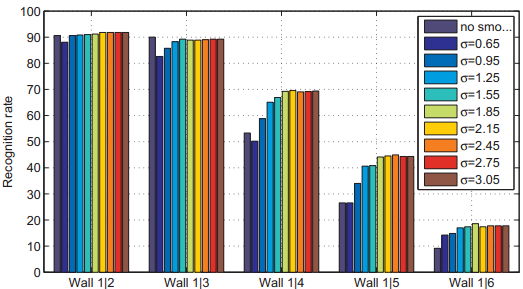
\includegraphics[scale=1]{pict/02/brief/sigma_comp.png}
\caption{Skuteczność rozpoznawania deskryptorów w zależności od stopnia wstępnego rozmycia obrazu}
\label{fig:brief_sigma_comp}
\end{figure}


Twórcy algorytmu zdecydowali się na zastosowanie rozmycia Gaussa. W trakcie prac nad algorytmem badano wpływ promienia rozmycia na jakość deskryptora i jego wydajność. Na zbiorze testowym Mikołajczyka\footnote{Zbiór testowy Mikołajczyka jest szerzej omówiony w rozdziale poświęconym badaniom} przetestowano promienie o zakresie od 0 do 3. Jak pokazuje wykres \ref{fig:brief_promien} w przedziale promieni od 1 do 3 jakość jest bardzo zbliżona. Finalnie w algorytmie zastosowano dyskretne jądro rozmycia o wartości $\sigma = 2 $ i rozmiarze 9 na 9 pikseli.

\subsection{Wybór testowanych par punktów}
Kluczowe znaczenie dla jakości generowanych deskryptorow, ma dobór par punktów poddawanych testowaniu. Od wyboru metody ich losowania zależy stopień powtarzalności i odporności desktyptora na rotacje. 

W trakcie prac nad algorytmem autorzy przetestowali 5 sposobów selekcji par:
\begin{enumerate}
\item[G I] Lokalizacja punktów \textbf{X} i \textbf{Y} ma rozkład jednostajny na przedziale $(-\frac{S}{2},\frac{S}{2})$. Początek układu współrzędnych umiejscowiony jest w punkcie centralnym badanago obszaru $S\times S$. 
\item[G II] Zbiory punktów \textbf{X} i \textbf{Y} mają rozkład normalny o wartości oczekiwanej 0 i wariancji $\frac{S^2}{25}$. Wartość wariancji została dobrana eksperymentalnie i dla przedstawionej metody zapewnia najwyższy współczynnik rozpoznawalności.
\item[G III] W przypadku tej metody próbkowanie odbywa się 2 etapowo. W pierwszej kolejności z rozkładem normalnym o wartości oczekiwanej 0 i wariancji $\frac{S^2}{25}$ wybierane są punkty \textbf{X}. Punkty \textbf{Y} są lokalizowane w otoczeniu odpowiadających im punktów $x_i$.  \textbf{Y} ma rozkład normalny o wartości oczekiwanej $x_i$ i wariancji $\frac{S^2}{100}$. W przypadku lokalizacja punktu $y_i$ wypada poza badany obszar $S\times S$ przypisuje mu się położenie na krawędzi. Zastosowana metoda powoduje, że badane pary są badane w sposób bardziej lokalny. Podobnie jak w poprzedniej metodzie wartości wariancji zostały dobrane eksperymentalnie.
\item[G IV] Punkty $x_i$ i $y_i$ są wybierane w sposób losowy z dyskretnego zbioru zgrubnych współrzędnych biegunowych.
\item[G V] Wszystkie punkty $x_i$ znajdują się w początku układu współrzednych a punkty $y_i$ lokalizowane są na liniach zgrubnych współrzędnych biegunowych.
\end{enumerate}

Zaproponowane metody próbkowania zostały przebadane na zbiorze testowym Mikołajczyka. Rezultaty tych badań przedstawione zostały na wykresie \ref{fig:brief_G_comp}. Otrzymane wyniki dowodzą wysokiej skuteczności metod opartych o losowy dobór par. Na ich tle wyjątkowo słabo wypada regularna i symetryczna metoda G V. W ostatecznej wersji algorytmu zdecydowano się zastosować strategie próbkowania G II.
\begin{figure}
\centering

\subfigure[G I]{
\includegraphics{pict/02/brief/G1.png}
}
\subfigure[G II]{
\includegraphics{pict/02/brief/G2.png}
}
\subfigure[G III]{
\includegraphics{pict/02/brief/G3.png}
}
\subfigure[G IV]{
\includegraphics{pict/02/brief/G4.png}
}
\subfigure[G V]{
\includegraphics{pict/02/brief/G5.png}
}
\caption{Przegląd metod losowania par punktów do testu binarnego}
\label{fig:brief_dist}
\end{figure}

\begin{figure}
\centering
\includegraphics[scale=1]{pict/02/brief/G_comp.png}
\caption{Skuteczność metod losowania par badana na zbiorze Mikołajczka WALL}
\label{fig:brief_G_comp}
\end{figure}

\FloatBarrier
\newpage
\section{Algorytm ORB}
Algorytm ORB jest rozwinięciem wcześniej omówionych algorytmów: FAST i BRIEF. Został on opracowany podobnie jak algorytm STAR w laboratorium robotyki Willow Garrage \cite{ORB11}. 

\subsection{Lokalizowanie punktów charakterystycznych}
Do lokalizowania punktów charakterystycznych algorytm ORB wykorzystuje zmodyfikowany detektor FAST. Jedna z modyfikacji polega na dodaniu do lokalizowanego punktu składowej określającej jego orientacje, dlatego nowy detektor nazwano oFAST (od ang. oriented FAST).


\begin{figure}
\centering
\includegraphics[width=0.8\textwidth]{pict/02/orb/orb_wykres_2.png}
\caption{podpis}
\label{fig:orb_wykres_2}
\end{figure}

\begin{figure}
\centering
\includegraphics[width=0.8\textwidth]{pict/02/orb/orb_wykres_3.png}
\caption{podpis}
\label{fig:orb_wykres_3}
\end{figure}


\begin{figure}
\centering
\includegraphics[width=0.8\textwidth]{pict/02/orb/orb_wykres_4.png}
\caption{podpis}
\label{fig:orb_wykres_4}
\end{figure}


\begin{figure}
\centering
\includegraphics[width=0.8\textwidth]{pict/02/orb/orb_wykres_5.png}
\caption{podpis}
\label{fig:orb_wykres_5}
\end{figure}



\begin{figure}
\centering
\includegraphics[width=0.8\textwidth]{pict/02/orb/orb_wykres_6.png}
\caption{podpis}
\label{fig:orb_wykres_6}
\end{figure}


\begin{figure}
\centering
\includegraphics[width=0.8\textwidth]{pict/02/orb/orb_wykres_7.png}
\caption{podpis}
\label{fig:orb_wykres_7}
\end{figure}


\begin{figure}
\centering
\includegraphics[width=0.8\textwidth]{pict/02/orb/orb_wykres_8.png}
\caption{podpis}
\label{fig:orb_wykres_8}
\end{figure}

Pierwszym krokiem w działaniu algorytmu jest "zgrubne" zlokalizowanie punktów charakterystycznych. Realizuje się to za pomocą detektora FAST-9, gdzie 9 oznacza ilość ciągłych pikseli w okręgu lokalizującym róg.

Oryginalny algorytm FAST nie dostarcza żadnej miary jakości zlokalizowanego rogu,  skutkiem czego jest bardzo wrażliwy na zakłócenia spowodowane odpowiedzią krawędziową. W efekcie bardzo często dostajemy bardzo dużą liczbę punktów charakterystycznych, niestety o słabej jakości. 

Rozwiązaniem powyższego problemu jest zastosowanie detektora Harrisa do oceniania punktów charakterystycznych. Algorytm ORB jako jeden z argumentów przyjmuje pożądaną liczbę punktów charakterystycznych oznaczoną przez N. Znając liczbę N algorytm tak ustala się wartość progu miary Harrisa aby uzyskać zbiór punktów, których ilość przekracza N. Następnie zbiór ten jest sortowany i wybiera się z niego N najlepszych punktów. W zastosowaniach praktycznych wartość liczby N ustala się najczęściej na 500. Zwiększenie tej liczby powoduje otrzymanie większej liczby punktów charakterystycznych, ale często gorszej jakości i nachodzące na punkty z grupy pięciuset.

Kolejnym wadę algorytmu FAST jest jego wrażliwość na skalowanie obrazu. W przypadku detektora oFAST zastosowano omawiany wcześniej mechanizm piramidy skalo-przestrzennej.

Do określenia orientacji rogu będącego punktem charakterystycznym zastosowano miarę intensywności środka ciężkości \cite{centroid}. Metoda ta zakłada, że intensywność rogu jest przesunięta względem jego środka. Wektor przesunięcia jest używany do określenie orientacji punktu charakterystycznego. 

Definiując dla badanego wycinka momenty jako:
\begin{equation}
m_{pq} = \sum\limits_{x,y} x^p y^q I(x,y)
\end{equation}
i środek ciężkości:
\begin{equation}
C = \left(\frac{m_{10}}{m_{00}},\frac{m_{01}}{m_{00}}\right)
\end{equation}
możemy skonstruować wektor $\overrightarrow{OC}$ zaczepiony w środku rogu i skierowany w stronę środka ciężkości. Orientacje tego wektora możemy w prosty sposób obliczyć z zależności:
\begin{equation}
\theta = atan2(m_{01},m_{10})
\end{equation}

Aby poprawić stabilność zaprezentowanej miary na rotacje, punkty $x$ i $y$ są wybierane z kołowego obszaru o promieniu $r$. W praktyce oznacza to, że $r$ reprezentuje rozmiar badanego wycinka a współrzędne $x$ i $y$ zawierają się w przedziale [-r,r]. W sytuacji gdy wartość momentu badanego odcinka |C| wynosi 0 algorytm zachowuje się w sposób niestabilny. W przypadku punktów lokalizowanych przez algorytm FAST jest to jednak bardzo rzadki przypadek.

Zaprezentowana metoda została porównana z metodami bazującymi na gradiencie obrazu, BIN i MAX. Metoda MAX wybiera największa składową gradientu w obrębie badanego punktu. Metoda BIN podobnie jak w algorytmie SIFT i jest oparta o histogram reprezentujący wszystkie składowe gradientu. Jak pokazuje wykres \ref{fig:orb_bin_max} metoda oparta o środek ciężkości jest o znacznie bardziej odporna na zakłócenia.
\subsection{Budowa deskryptora}
Do opisu zlokalizowanych cech wykorzystano ulepszoną zmodyfikowaną wersje deskryptora Steered BRIEF nazwaną rBRIEF. 

Steered Brief jest rozwinięciem opisanego wcześniej deskryptora BRIEF. Oryginalny deskryptor BRIEF jest bardzo wrażliwy na rotacje \ref{fig:orb_compare_desc}. Pewnym rozwiązaniem, aczkolwiek bardzo nieoptymalnym, jest zaproponowane przez autorów algorytmu BRIEF wyliczenie grupy obróconych względem siebie deskryptorów. Znacznie lepszym rozwiązaniem dostrojenie deskryptora BRIEF do orientacji punktu charakterystycznego. Deskryptor BRIEF jest generowany przez $n$ testów binarny dla zbioru par punktów ($x_i$,$y_i$). Zbiór ten jest opisany przez macierz $\textbf{S}$:
\begin{equation}
\textbf{S} = \left(\begin{array}{ccccccc}
x_1 & , & x_2 & , & ... & , & x_n \\
y_1 & , & y_2 & , & ... & , & y_n \\
\end{array}
\right)
\end{equation} 

Na podstawie obliczonej wcześniej orientacji punktu charakterystycznego $\theta$ i odpowiadającej jej macierzy rotacji $\textbf{R}_{\theta}$, konstruowany jest "ukierunkowany" zbiór testowy $\textbf{S}_{\theta}$:

\begin{equation}
\textbf{S}_\theta = \textbf{R}_\theta \textbf{S}
\end{equation}

Otrzymany zbiór jest poddawany temu samemu testowi jak w przypadku oryginalnego algorytmu BRIEF (wzór \ref{eqn:brief_test}).

W celu usprawnienia pracy algorytmu orientacje punktów charakterystycznych poddawane są kwantyzacji. Dla zakresu $360^o$ przyjęto się 30 przedziałów $12^o$ do których może zostać zakwalifikowana orientacja punktu. Każdy z przedziałów posiada własny wzorzec punktów poddawanych testom.

Jedną z niewątpliwych zalet algorytmu BRIEF jest to że każdy bit jego deskryptora ma dużą wariancje i wartość średnią na poziomie $0,5$. Wykres \ref{fig:orb_spread} prezentuje rozrzut wartości średniej dla typowego gaussowskiego wzorca 256 bitowego deskryptora BRIEF dla zbioru 100 tysięcy punktów charakterystycznych. Wartość średnia $0,5$ daje największą wariancje próbkowania na poziomie $0,25$ dla pojedynczego bitu. Zastosowanie "ukierunkowanego" algorytmu BRIEF powoduje przesunięcie wartości średniej w stronę rozkładu typowego dla wzorca odpowiadającego danemu kątowi orientacji. Powoduje to zbytnie upodobnienie się deskryptorów punktów zakwalifikowanych do tego samego przedziału orientacji.

Wysoka wariancje czyni deskryptory bardziej dyskryminacyjnymi co jest pożądanym zjawiskiem, gdyż generuje bardziej zróżnicowane odpowiedzi dla punktów o podobnych parametrach. 

Kolejnym ważnym aspektem  jest również to aby kolejne bity deskryptora były ze sobą nieskorelowane. Autorzy algorytmu dla badanego zbioru 100 tysięcy punktów dokonali analizy głównych składowych (ang. PCA) otrzymywanych deskryptorów. Wyniki tego badania przedstawia wykres \ref{fig:orb_wykres_4}. Na podstawie analizy wykreślono 40 najwyższych wartości własnych, po których zarówno deskyptory BRIEF jak steered BRIEF się pokrywają. Obie motody wykazują wysokie wejściowe wartości własne, wskazujące na korelacje testów binarnych. Większość informacji jest zawarta w pierwszych 15 komponentach. Algorytm steered BRIEF ma znacznie mniejszą wariancję, aczkolwiek przy mniejszych wartościach własnych przestaje być dyskryminacyjnym. Na podstawie tego można stwierdzić, że BRIEF zawdzięcza swoja dobre wyniki losowej orientacji punktów charakterystycznych.

Innym niekorzystnym efektem towarzyszącym deskryptorowi steered BRIEF jest zmniejszenie dystansu miedzy punktami pokrywającymi się i odstającymi co przedstawiono na wykresie \ref{fig:orb_wykres_5}. Może to powodować nie pożądane nachodzenie na siebie punktów poprawnych i złych, a co za tym idzie powodować fałszywe dopasowania.

Aby zapobiec opisanym zjawiskom spadku wariancji i wzrostu korelacji pomiędzy testami, autorzy algorytmu zaproponowali metodę uczenia służącą wyborowi dobrego podzbioru binarnych testów.

W zaproponowanej metodzie na zbioru obrazów PASCAL 2006 \cite{pascal} przygotowano zbiór uczący zawierający około 300 tysięcy punktów charakterystycznych. Następnie dla okna o wymiarach $31\times31$ pikseli przygotowano kombinacje wszystkich możliwych binarnych testów. Każdy test jest jest wykonywanywany na parze mniejszego okien $5\times$. Zapisując szerokość dużego okna jako $w_p = 31$ i szerokość małego okna jako $w_t = 5$ otrzymujemy liczbę $N = (w_p - w_t)^2$ oznaczającą liczbę możliwych małych okien. Wybierając 2 okna do pojedyńczego badania otrzymujemy zbiór ${N\choose 2}$ testów. Eliminując testy nakładające się na siebie otrzymujemy zbiór 205590 porównań.

Przygotowany zbiór uczący poddano badaniu nastepującemu algorytmowi:
\begin{enumerate}
\item Wszystkie obrazy zbioru uczącego przetestowano wszystkimi kombinacjami testów.
\item Testy zostały uporządkowane na podstawie odległości wartości średniej od wartości $0,5$ i zawarte w wektorze \textbf{T}.
\item Następnie wektor \textbf{T} jest poddawany przeszukiwaniu zachłannemu:
\begin{enumerate}
\item Pierwszy test wektora \textbf{T} jest kopiowany do 256 wymiarowego wektora \textbf{R} i usuwany ze zbioru \textbf{T}.
\item Kolejny test ze zbioru \textbf{T} jest porównywany ze wszystkimi testami znajdującymi w wektorze \textbf{R}. W sytuacji gdy wartość absolutna korelacji między testami jest mniejsza niż zadany próg, test zostaje przeniesiony do zbioru wektora \textbf{R}.
\item Punkt (b) jest powtarzany aż do momenty, w którym w wektor \textbf{R} będzie posiadał 256 elementów. W sytuacji niespełnienia warunku stopu i wyczerpania się elementów wektora \textbf{T} wartość progu jest podnoszona i algorytm powtarza swoje działanie.
\end{enumerate}
\end{enumerate}
Wynik działania tego algorytmu został nazwany rBRIEF. Algorytm ten ma znacząco lepsze parametry wariancji i korelacji niż algorytm steered BRIEF. Jak przedstawia wykres \ref{fig:orb_wykres_4} wygenerowany deskryptor ma wartości własne glównych składowych są wyższe i zmniejszają się znacznie wolniej niż w przypadku algorytmów steered BRIEF i BRIEF. Badania przeprowadzone przez autorów algorytmów wykazują ponadto wysoką odporność na rotacje \ref{fig:orb_wykres_7}.
\part{Badania}
\chapter{Opis badań}
Omówione w cześci teoretycznej algorytmy zostały przebadane pod kątem efektywności działania.
W tym celu został napisany program komputerowy, którego szerszy opis można znaleść w dodatku \ref{dodatek_program}.
\FloatBarrier 
\section{Badane algorytmy}
Problem poprawnego rozpoznawania obrazów opartego o cechy charakterystyczne można zdekomponować na dwa mniejsze jakimi są:
\begin{itemize}
\item lokalizowanie punktów charakterystycznych,
\item opisywanie punktów charakterystycznych.
\end{itemize}
Oba aspekty są kluczowe dla realizacji postawionego zadania, a efekt finalny jest wypadkową pracy detektorów i deskryptorów. Z tego względu przyjęto założenie, że algorytmy kompletne tj. zawierające zarówno detektor jak i deskryptor zostaną zestawione z algorytmami mieszanymi. W przypadku algorytmów nie posiadających własnych mechanizmów opisu cech, pulę dostępnych deskryptorów wzbogacono o metody algorytmów kompletnych. Zastosowane podejście pozwoliło porównać ze sobą niezależnie stosowane detektory i deskryptory.
Postanowiono przebadać następujące algorytmy:
\begin{itemize}
\item ORB
\item SIFT
\item SURF
\item detektor STAR + deskryptor BRIEF
\item detektor STAR + deskryptor ORB (\textit{wł. rBRIEF})
\item detektor STAR + deskryptor SIFT
\item detektor STAR + deskryptor SURF
\item detektor FAST + deskryptor BRIEF $^1$
\item detektor FAST + deskryptor ORB (\textit{wł. rBRIEF}) $^1$
\item detektor FAST + deskryptor SIFT $^1$
\item detektor FAST + deskryptor SURF $^1$
\end{itemize}
\footnote{Pierwsze testy wykazały jednakże, że ilość punktów charakterystycznych lokalizowanych przez algorytm FAST jest zbyt duża, aby można było dokonać dopasowania w rozsądnym czasie pracy maszyny.W związku z powyższym badany zrezygnowano z opisywania i dopasowywania cech lokalizowanych przez ten algorytm}

\FloatBarrier
\section{Kryteria badań}
W porównywaniu algorytmów wzięto pod uwagę następujące kryteria:
\begin{itemize}
\item ilość lokalizowanych cech
\item czas potrzebny na zlokalizowanie pojedynczego punktu charakterystycznego
\item czas potrzebny na wygenerowanie deskryptora pojedynczego punktu charakterystycznego
\item powtarzalność zlokalizowanych cech
\item procent poprawnych dopasowań
\end{itemize}



Ze względu na to że algorytmy różnią się czasem działania i ilością lokalizowanych cech w rożnych obrazach, wszystkie kryteria czasowe zdecydowano się odnieść do pojedynczego punktu.


Powtarzalność zlokalizowanych cech jest rozumiana jako:
\begin{equation}
p_{AB}  = \frac{d_{AB}}{i_{AB}}
\end{equation}
gdzie:\\
$p_{AB}$ - powtarzalność lokalizowanych cech między obrazami A i B\\
$d_{AB}$ - ilość dopasowanych cech między obrazami A i B metodą k najbliższych sąsiadów\\
$i_{AB}$ - średnia arytmetyczna ilości punktów zlokalizowanych w obrazach A i B\\


Do oceny jakości parowania cech wykorzystano algorytm RANSAC \cite{ransac}. Pozwala on wyeliminować błędne dopasowania nie pasujące do estymowanego wzorca. Za procent poprawnych dopasowań rozumiemy stosunek ilość par punktów po zastosowaniu algorytmu RANSAC do ilości wstępnie dopasowanych punktów.
\FloatBarrier
\section{Zbiory testowe}
Do oceny pracy algorytmów wykorzystano dwa zbiory testowe:
\begin{itemize}
\item zbiór testowy Mikołajczyka
\item autorski zbiór testowy przedstawiający obrazy skalne
\end{itemize}
W skład obu zbiorów wchodzą zestawy obrazów pogrupowane wg, przekształceń takich jak rotacja, zmiana skali, zmiana oświetlenie lub położenia obserwatora. Każdy pojedynczy zestaw składa się z 6 zdjęć. Pierwsze zdjęcie jest obiektem referencyjnym względem którego dokonywane są dopasowania. Kolejne zdjęcia zestawu są poddawane coraz mocniejszym przekształceniom.

\FloatBarrier
\chapter{Zbiór testowy Mikołajczyka}
Zbiór testowy Mikołajczyka to opracowany przez doktora Krystiana Mikołajczyka zespół zestawów obrazów testowych służących ocenie afinicznych, kowariantnych cech. Zawiera on przekształcenia takie jak:
\begin{itemize}
\item zmiana położenia obserwatora
\item zmiana skali 
\item rotacja
\item zmiana oświetlenia
\item rozmycie
\item kompresja JPEG
\end{itemize}
Oryginalny zbiór zawiera 8 zestawów zawierające powyższe transformacje. Zbiory dotyczące położenia obserwatora, skali i rozmycia są zdublowane. Uczyniono to aby uniezależnić ocenę jakości pracy z  przekształcenie od charakterystyki obrazu. W przeprowadzonych badaniach zrezygnowano z testowania odporności algorytmów na kompresje JPEG. Ze względu na fakt, że zbiór Mikołajczyka jest często wykorzystywany w badaniach, zdecydowano się zachować angielskie nazewnictwo zestawów. Zbiór jest dostępny w internecie na stronie \textit{http://www.robots.ox.ac.uk/~vgg/research/affine/}.
\FloatBarrier
\newpage
\section{Rozmycie obrazu}
\FloatBarrier
\subsection{BIKES}

\begin{figure}[!htb]
\begin{center}

\subfigure[BIKES-1]{
\includegraphics[width=5cm]{pict/mikolajczyk/bikes/img1.jpg}
}
\subfigure[BIKES-2]{
\includegraphics[width=5cm]{pict/mikolajczyk/bikes/img2.jpg}
}
\subfigure[BIKES-3]{
\includegraphics[width=5cm]{pict/mikolajczyk/bikes/img3.jpg}
}
\subfigure[BIKES-4]{
\includegraphics[width=5cm]{pict/mikolajczyk/bikes/img4.jpg}
}
\subfigure[BIKES-5]{
\includegraphics[width=5cm]{pict/mikolajczyk/bikes/img5.jpg}
}
\subfigure[BIKES-6]{
\includegraphics[width=5cm]{pict/mikolajczyk/bikes/img6.jpg}
}
\caption{BIKES - zbiór obrazów testowych}
\label{fig:bikes_set}
\end{center}
\end{figure}



% Table generated by Excel2LaTeX from sheet 'm.bikes F'
\begin{table}[htbp]
  \centering
  \caption{BIKES - ilość wyszukanych cech}
    \begin{tabular}{|c|r|r|r|r|r|}\hline
    
    obraz & \textbf{ORB} & \textbf{SIFT} & \textbf{SURF} & \textbf{STAR} & \textbf{FAST} \\\hline
    
   
    1 & 500 & 1014 & 12911 & 586 & 10702 \\
    2 & 500 & 1062 & 8974 & 362 & 3128 \\
    3 & 500 & 1159 & 8100 & 290 & 2247 \\
    4 & 485 & 839 & 7151 & 181 & 1129 \\
    5 & 420 & 596 & 6344 & 139 & 675 \\
    6 & 366 & 473 & 5751 & 118 & 500 \\\hline
    \textbf{średnia} & \textbf{462} & \textbf{857} & \textbf{8205} & \textbf{279} & \textbf{3064} \\
    \hline
    \end{tabular}%
  \label{tab:bikes_f1}%
\end{table}%


\begin{figure}
\centering
\includegraphics[width=0.8\textwidth]{pict/mikolajczyk/bikes/f1.png}
\caption{BIKES - ilość wyszukanych cech}
\label{fig:bikes_f1}
\end{figure}


% Table generated by Excel2LaTeX from sheet 'm.bikes F'
\begin{table}[htbp]
  \centering
  \caption{BIKES - czas lokalizowania pojedynczego punktu charakterystycznego}
    \begin{tabular}{|c|c|c|c|c|c|}
    \hline
    obraz & \textbf{ORB} & \textbf{SIFT} & \textbf{SURF} & \textbf{STAR} & \textbf{FAST} \\
    \hline
   
    1 & 0,080 & 0,179 & 0,156 & 0,109 & 0,001 \\
    2 & 0,062 & 0,171 & 0,169 & 0,182 & 0,002 \\
    3 & 0,060 & 0,153 & 0,173 & 0,217 & 0,002 \\
    4 & 0,056 & 0,204 & 0,179 & 0,348 & 0,003 \\
    5 & 0,060 & 0,282 & 0,185 & 0,453 & 0,003 \\
    6 & 0,066 & 0,340 & 0,191 & 0,542 & 0,004 \\\hline
    \textbf{średnia} & \textbf{0,064} & \textbf{0,222} & \textbf{0,175} & \textbf{0,309} & \textbf{0,002} \\
   \hline
    \end{tabular}%
  \label{tab:bikes_f2}%
\end{table}%


\begin{figure}
\centering
\includegraphics[width=0.8\textwidth]{pict/mikolajczyk/bikes/f2.png}
\caption{BIKES - czas lokalizowania pojedynczego punktu charakterystycznego}
\end{figure}

% Table generated by Excel2LaTeX from sheet 'm.bikes F'
\begin{table}[htbp]
  \centering
  \caption{BIKES - czas generowania pojedynczego deskryptora punktu charakterystycznego}
    \begin{tabular}{|c|c|c|c|c|c|c|c|}\hline

    obraz & \textbf{ORB} & \textbf{SIFT} & \textbf{SURF} & \textbf{ST-BRIEF} & \textbf{ST-ORB} & \textbf{ST-SIFT} & \textbf{ST-SURF} \\\hline

    - & [ms] & [ms] & [ms] & [ms] & [ms] & [ms] & [ms] \\\hline
    1 & 0,092 & 0,300 & 0,193 & 0,015 & 0,019 & 1,109 & 0,094 \\
    2 & 0,090 & 0,293 & 0,201 & 0,019 & 0,025 & 1,561 & 0,099 \\
    3 & 0,090 & 0,283 & 0,199 & 0,017 & 0,031 & 1,803 & 0,103 \\
    4 & 0,093 & 0,344 & 0,194 & 0,022 & 0,044 & 2,420 & 0,116 \\
    5 & 0,107 & 0,424 & 0,195 & 0,029 & 0,050 & 3,201 & 0,129 \\
    6 & 0,120 & 0,474 & 0,198 & 0,025 & 0,059 & 3,873 & 0,136 \\\hline
    \textbf{średnia} & \textbf{0,099} & \textbf{0,353} & \textbf{0,197} & \textbf{0,021} & \textbf{0,038} & \textbf{2,328} & \textbf{0,113} \\\hline
    

    \end{tabular}%
  \label{tab:bikes_f3}%
\end{table}%


\begin{figure}
\centering
\includegraphics[width=0.8\textwidth]{pict/mikolajczyk/bikes/f3.png}
\caption{BIKES - czas generowania pojedynczego deskryptora punktu charakterystycznego}
\label{fig:bikes_f3}
\end{figure}


% Table generated by Excel2LaTeX from sheet 'm.bikes M'
\begin{table}[htbp]
  \centering
  \caption{BIKES - powtarzalność wykrywanych cech}
    \begin{tabular}{|c|c|c|c|c|c|c|c|}\hline

    obrazy & \textbf{ORB} & \textbf{SIFT} & \textbf{SURF} & \textbf{ST-BRIEF} & \textbf{ST-ORB} & \textbf{ST-SIFT} & \textbf{ST-SURF} \\\hline

    -  & [\%] & [\%] & [\%] & [\%] & [\%] & [\%] & [\%] \\\hline
    1|2 & 44 & 50 & 38 & 55 & 59 & 61 & 27 \\
    1|3 & 38 & 39 & 25 & 43 & 42 & 42 & 20 \\
    1|4 & 23 & 36 & 16 & 32 & 28 & 30 & 11 \\
    1|5 & 18 & 32 & 11 & 35 & 22 & 33 & 8 \\
    1|6 & 12 & 27 & 7 & 19 & 19 & 29 & 5 \\\hline
    \textbf{średnia} & \textbf{27} & \textbf{37} & \textbf{19} & \textbf{37} & \textbf{34} & \textbf{39} & \textbf{14} \\\hline
    

    \end{tabular}%
  \label{tab:bikes_m1}%
\end{table}%


\begin{figure}
\centering
\includegraphics[width=0.8\textwidth]{pict/mikolajczyk/bikes/m1.png}
\caption{BIKES - powtarzalność wykrywanych cech}
\label{fig:bikes_m1}
\end{figure}

% Table generated by Excel2LaTeX from sheet 'm.bikes M'
\begin{table}[htbp]
  \centering
  \caption{BIKES - procent poprawnych dopasowań}
    \begin{tabular}{|c|c|c|c|c|c|c|c|}\hline
    obrazy & \textbf{ORB} & \textbf{SIFT} & \textbf{SURF} & \textbf{ST-BRIEF} & \textbf{ST-ORB} & \textbf{ST-SIFT} & \textbf{ST-SURF} \\\hline
     - & [\%] & [\%] & [\%] & [\%] & [\%] & [\%] & [\%] \\\hline
   1|2 & 64 & 88 & 66 & 59 & 65 & 73 & 59 \\
    1|3 & 58 & 74 & 52 & 54 & 51 & 55 & 57 \\
    1|4 & 37 & 62 & 50 & 32 & 40 & 41 & 39 \\
    1|5 & 41 & 69 & 31 & 38 & 32 & 40 & 39 \\
    1|6 & 44 & 49 & 30 & 23 & 28 & 37 & 32 \\\hline
    \textbf{średnia} & \textbf{49} & \textbf{68} & \textbf{46} & \textbf{41} & \textbf{43} & \textbf{49} & \textbf{45} \\\hline
    
    \end{tabular}%
  \label{tab:bikes_m2}%
\end{table}%


\begin{figure}
\centering
\includegraphics[width=0.8\textwidth]{pict/mikolajczyk/bikes/m2.png}
\caption{BIKES - procent poprawnych dopasowań}
\label{fig:bikes_m2}
\end{figure}








\newpage
\FloatBarrier
\subsection{TREES}

\begin{figure}[!htb]
\begin{center}
\subfigure[TREES-1]{
\includegraphics[width=5cm]{pict/mikolajczyk/trees/img1.jpg}
}
\subfigure[TREES-2]{
\includegraphics[width=5cm]{pict/mikolajczyk/trees/img2.jpg}
}
\subfigure[TREES-3]{
\includegraphics[width=5cm]{pict/mikolajczyk/trees/img3.jpg}
}
\subfigure[TREES-4]{
\includegraphics[width=5cm]{pict/mikolajczyk/trees/img4.jpg}
}
\subfigure[TREES-5]{
\includegraphics[width=5cm]{pict/mikolajczyk/trees/img5.jpg}
}
\subfigure[TREES-6]{
\includegraphics[width=5cm]{pict/mikolajczyk/trees/img6.jpg}
}
\caption{TREES - zbiór obrazów testowych}
\label{fig:trees_set}
\end{center}
\end{figure}
\FloatBarrier


% Table generated by Excel2LaTeX from sheet 'm.trees F'
\begin{table}[htbp]
  \centering
  \caption{TREES - ilość wyszukanych cech}
    \begin{tabular}{|c|r|r|r|r|r|}\hline
    
    obraz & \textbf{ORB} & \textbf{SIFT} & \textbf{SURF} & \textbf{STAR} & \textbf{FAST} \\\hline
    
   
    1 & 500 & 2941 & 11343 & 2539 & 34024 \\
    2 & 500 & 2848 & 12563 & 2536 & 38235 \\
    3 & 500 & 3363 & 10377 & 2846 & 28516 \\
    4 & 500 & 4150 & 8613 & 2398 & 16582 \\
    5 & 500 & 4244 & 8022 & 1383 & 11716 \\
    6 & 500 & 2709 & 6605 & 824 & 7883 \\\hline
    \textbf{średnia} & \textbf{500} & \textbf{3376} & \textbf{9587} & \textbf{2088} & \textbf{22826} \\
   \hline
    \end{tabular}%
  \label{tab:trees_f1}%
\end{table}%


\begin{figure}
\centering
\includegraphics[width=0.8\textwidth]{pict/mikolajczyk/trees/f1.png}
\caption{TREES - ilość wyszukanych cech}
\label{fig:trees_f1}
\end{figure}


% Table generated by Excel2LaTeX from sheet 'm.trees F'
\begin{table}[htbp]
  \centering
  \caption{TREES - czas lokalizowania pojedynczego punktu charakterystycznego w obrazach z zestawu TREES}
    \begin{tabular}{|c|c|c|c|c|c|}
    \hline
    obraz & \textbf{ORB} & \textbf{SIFT} & \textbf{SURF} & \textbf{STAR} & \textbf{FAST} \\
    \hline
    -  & [ms] & [ms] & [ms] & [ms] & [ms] \\\hline
    1 & 0,162 & 0,077 & 0,162 & 0,027 & 0,001 \\
    2 & 0,172 & 0,088 & 0,158 & 0,026 & 0,001 \\
    3 & 0,158 & 0,067 & 0,165 & 0,024 & 0,001 \\
    4 & 0,130 & 0,058 & 0,173 & 0,028 & 0,002 \\
    5 & 0,102 & 0,058 & 0,175 & 0,047 & 0,002 \\
    6 & 0,078 & 0,085 & 0,185 & 0,078 & 0,001 \\\hline
    \textbf{średnia} & \textbf{0,134} & \textbf{0,072} & \textbf{0,170} & \textbf{0,038} & \textbf{0,001} \\
   \hline
    \end{tabular}%
  \label{tab:trees_f2}%
\end{table}%


\begin{figure}
\centering
\includegraphics[width=0.8\textwidth]{pict/mikolajczyk/trees/f2.png}
\caption{TREES - czas lokalizowania pojedynczego punktu charakterystycznego}
\label{fig:trees_f2}
\end{figure}

% Table generated by Excel2LaTeX from sheet 'm.trees F'
\begin{table}[htbp]
  \centering
  \caption{TREES - czas generowania pojedynczego deskryptora punktu charakterystycznego}
    \begin{tabular}{|c|c|c|c|c|c|c|c|}\hline

    obraz & \textbf{ORB} & \textbf{SIFT} & \textbf{SURF} & \textbf{ST-BRIEF} & \textbf{ST-ORB} & \textbf{ST-SIFT} & \textbf{ST-SURF} \\\hline

    - & [ms] & [ms] & [ms] & [ms] & [ms] & [ms] & [ms] \\\hline
    1 & 0,064 & 0,207 & 0,209 & 0,012 & 0,012 & 0,460 & 0,083 \\
    2 & 0,064 & 0,210 & 0,203 & 0,012 & 0,012 & 0,442 & 0,084 \\
    3 & 0,064 & 0,197 & 0,209 & 0,012 & 0,011 & 0,516 & 0,084 \\
    4 & 0,064 & 0,188 & 0,213 & 0,012 & 0,012 & 0,620 & 0,085 \\
    5 & 0,064 & 0,200 & 0,204 & 0,012 & 0,014 & 1,091 & 0,093 \\
    6 & 0,064 & 0,240 & 0,202 & 0,013 & 0,017 & 1,602 & 0,103 \\\hline
    \textbf{średnia} & \textbf{0,064} & \textbf{0,207} & \textbf{0,207} & \textbf{0,012} & \textbf{0,013} & \textbf{0,789} & \textbf{0,089} \\\hline
    

    \end{tabular}%
  \label{tab:trees_f3}%
\end{table}%


\begin{figure}
\centering
\includegraphics[width=0.8\textwidth]{pict/mikolajczyk/trees/f3.png}
\caption{TREES - czas generowania pojedynczego deskryptora punktu charakterystycznego}
\label{fig:trees_f3}
\end{figure}


% Table generated by Excel2LaTeX from sheet 'm.trees M'
\begin{table}[htbp]
  \centering
  \caption{TREES - powtarzalność wykrywanych cech}
    \begin{tabular}{|c|c|c|c|c|c|c|c|}\hline

    obrazy & \textbf{ORB} & \textbf{SIFT} & \textbf{SURF} & \textbf{ST-BRIEF} & \textbf{ST-ORB} & \textbf{ST-SIFT} & \textbf{ST-SURF} \\\hline

    -  & [\%] & [\%] & [\%] & [\%] & [\%] & [\%] & [\%] \\\hline
    1|2 & 18 & 18 & 11 & 38 & 12 & 38 & 3 \\
    1|3 & 25 & 15 & 9 & 32 & 9 & 32 & 2 \\
    1|4 & 13 & 8 & 4 & 20 & 4 & 18 & 1 \\
    1|5 & 6 & 5 & 3 & 18 & 5 & 9 & 1 \\
    1|6 & 3 & 4 & 1 & 14 & 2 & 3 & 0 \\\hline
    \textbf{średnia} & \textbf{13} & \textbf{10} & \textbf{6} & \textbf{24} & \textbf{6} & \textbf{20} & \textbf{1} \\\hline
   

    \end{tabular}%
  \label{tab:trees_m1}%
\end{table}%


\begin{figure}
\centering
\includegraphics[width=0.8\textwidth]{pict/mikolajczyk/trees/m1.png}
\caption{TREES - powtarzalność wykrywanych cech}
\label{fig:trees_m1}
\end{figure}

% Table generated by Excel2LaTeX from sheet 'm.trees M'
\begin{table}[htbp]
  \centering
  \caption{TREES - procent poprawnych dopasowań}
    \begin{tabular}{|c|c|c|c|c|c|c|c|}\hline
    obrazy & \textbf{ORB} & \textbf{SIFT} & \textbf{SURF} & \textbf{ST-BRIEF} & \textbf{ST-ORB} & \textbf{ST-SIFT} & \textbf{ST-SURF} \\\hline
     - & [\%] & [\%] & [\%] & [\%] & [\%] & [\%] & [\%] \\\hline
    1|2 & 43 & 45 & 50 & 56 & 71 & 62 & 33 \\
    1|3 & 71 & 47 & 40 & 63 & 62 & 67 & 30 \\
    1|4 & 57 & 35 & 28 & 41 & 35 & 51 & 16 \\
    1|5 & 31 & 30 & 18 & 41 & 23 & 38 & 6 \\
    1|6 & 33 & 23 & 13 & 33 & 14 & 20 & 4 \\\hline
    \textbf{średnia} & \textbf{47} & \textbf{36} & \textbf{30} & \textbf{47} & \textbf{41} & \textbf{48} & \textbf{18} \\\hline
    
    \end{tabular}%
  \label{tab:trees_m2}%
\end{table}%


\begin{figure}
\centering
\includegraphics[width=0.8\textwidth]{pict/mikolajczyk/trees/m2.png}
\caption{TREES - procent poprawnych dopasowań}
\label{fig:trees_m2}
\end{figure}
\FloatBarrier
\subsection{Dyskusja wyników}
Jak możemy zaobserwować na wykresach \ref{fig:bikes_f1} i \ref{fig:trees_f1} wraz ze wzrostem stopnia rozmycia obrazu maleje liczba lokalizowanych punktów charakterystycznych. Wśród ilości lokalizowanych punktów prym wiodą w zależności od scenerii algorytmy SURF i FAST, i to wśród ich wyników spadek ilości punktów jest najbardziej zauważalny. Algorytmy te generują o rząd wielkości więcej punktów niż pozostałe metody. Niestety jakość tych punktów pozostawia często wiele do życzenia, a ich ilość w sposób znaczący utrudnia proces dopasowywania. Rysunek \ref{tt13} przedstawia punkty wyszukane przez algorytm FAST w obrazach z zestawu TREES. Jak widzimy ich ilość w sposób znaczący zaciemnia obraz.

Większość algorytmów jest wrażliwa na stopień rozmycia, co przekłada się na czas lokalizowania punktów charakterystycznych. Na tym tle korzystnie wypada algorytm ORB, poprawiający swoje charakterystyki czasowe przy zachowanej stałej liczbie lokalizowanych punktów.

W przypadku generowania deskryptora punktu charakterystycznego większość algorytmów zachowuje względnie stałe wartości czasowe. Wyniki te mogą się nieznacznie różnić w zależności od analizowanej sceny. Wyjątkiem tu są dokładne deskryptory gradientowe SIFT. Wraz ze wzrostem rozmycia obserwujemy wzrost czasu potrzebnego na obliczenie deskryptora. Szczególnie dramatyczny wzrost ma miejsce w przypadku kombinacji deskryptora SIFT z detektorem STAR. Częściową tą wadę rekompensuje wysoka na tle innych algorytmów powtarzalność dopasowań.

Powtarzalność dopasowań dla wszystkich algorytmów spada wraz ze wzrostem rozmycia. Parametr ten w zależności od scenerii osiąga maksymalną wartość od 30 do 60 \%. Jak pokazują algorytmy są wrażliwe w przypadku rozmycia obrazów o dużej ilości drobnych, podobnych elementów jakimi są liście.

W przypadku obrazów o zróżnicowanych elementach najlepszy współczynnik trafnych dopasowań osiąga algorytm SIFT. W sytuacji gdy obraz wskutek rozmycia w znacznym stopniu staje się nieczytelny jak w przypadku obrazów TREES lepszą odpornością wykazują się algorytm ORB i kombinacja algorytmów STAR i BRIEF.







\begin{figure}
\centering
\includegraphics[width=0.8\textwidth]{pict/badania/trees_fast_1_3.png}
\caption{Zlokalizowane przez algorytm FAST punkty charakterystyczne w obrazach TREES-1 i TREES-3}
\label{tt13}
\end{figure}





\FloatBarrier
\section{Zmiana położenia obserwatora}
\FloatBarrier
\subsection{GRAFFITI}

\begin{figure}[!htb]
\begin{center}
\subfigure[GRAFFITI-1]{
\includegraphics[width=5cm]{pict/mikolajczyk/graff/img1.jpg}
}
\subfigure[GRAFFITI-2]{
\includegraphics[width=5cm]{pict/mikolajczyk/graff/img2.jpg}
}
\subfigure[GRAFFITI-3]{
\includegraphics[width=5cm]{pict/mikolajczyk/graff/img3.jpg}
}
\subfigure[GRAFFITI-4]{
\includegraphics[width=5cm]{pict/mikolajczyk/graff/img4.jpg}
}
\subfigure[GRAFFITI-5]{
\includegraphics[width=5cm]{pict/mikolajczyk/graff/img5.jpg}
}
\subfigure[GRAFFITI-6]{
\includegraphics[width=5cm]{pict/mikolajczyk/graff/img6.jpg}
}
\caption{GRAFFITI - zbiór obrazów testowych}
\label{fig:graffiti_set}
\end{center}
\end{figure}
\FloatBarrier


% Table generated by Excel2LaTeX from sheet 'm.graff F'
\begin{table}[htbp]
  \centering
  \caption{GRAFFITI - ilość wyszukanych cech}
    \begin{tabular}{|c|r|r|r|r|r|}\hline
    
    obraz & \textbf{ORB} & \textbf{SIFT} & \textbf{SURF} & \textbf{STAR} & \textbf{FAST} \\\hline
    
   
    1 & 500 & 1128 & 8444 & 878 & 6727 \\
    2 & 500 & 1296 & 8538 & 930 & 7567 \\
    3 & 500 & 1358 & 8869 & 1147 & 8579 \\
    4 & 500 & 1445 & 8888 & 973 & 11146 \\
    5 & 500 & 1500 & 9165 & 1164 & 10053 \\
    6 & 500 & 1478 & 9875 & 910 & 13459 \\\hline
    \textbf{średnia} & \textbf{500} & \textbf{1368} & \textbf{8963} & \textbf{1000} & \textbf{9589} \\
    \hline
    \end{tabular}%
  \label{tab:graffiti_f1}%
\end{table}%


\begin{figure}
\centering
\includegraphics[width=0.8\textwidth]{pict/mikolajczyk/graff/f1.png}
\caption{GRAFFITI - ilość wyszukanych cech}
\end{figure}


% Table generated by Excel2LaTeX from sheet 'm.graff F'
\begin{table}[htbp]
  \centering
  \caption{GRAFFITI - czas lokalizowania pojedynczego punktu charakterystycznego}
    \begin{tabular}{|c|c|c|c|c|c|}
    \hline
    obraz & \textbf{ORB} & \textbf{SIFT} & \textbf{SURF} & \textbf{STAR} & \textbf{FAST} \\
    \hline
    -  & [ms] & [ms] & [ms] & [ms] & [ms] \\\hline
    1 & 0,074 & 0,122 & 0,158 & 0,054 & 0,001 \\
    2 & 0,080 & 0,113 & 0,158 & 0,051 & 0,001 \\
    3 & 0,088 & 0,108 & 0,156 & 0,041 & 0,001 \\
    4 & 0,092 & 0,102 & 0,156 & 0,049 & 0,001 \\
    5 & 0,088 & 0,099 & 0,156 & 0,041 & 0,001 \\
    6 & 0,098 & 0,101 & 0,153 & 0,052 & 0,001 \\\hline
    \textbf{średnia} & \textbf{0,087} & \textbf{0,108} & \textbf{0,156} & \textbf{0,048} & \textbf{0,001} \\
    \hline
    \end{tabular}%
  \label{tab:graffiti_f2}%
\end{table}%


\begin{figure}
\centering
\includegraphics[width=0.8\textwidth]{pict/mikolajczyk/graff/f2.png}
\caption{GRAFFITI - czas lokalizowania pojedynczego punktu charakterystycznego}
\end{figure}

% Table generated by Excel2LaTeX from sheet 'm.graff F'
\begin{table}[htbp]
  \centering
  \caption{GRAFFITI - czas generowania pojedynczego deskryptora punktu charakterystycznego}
    \begin{tabular}{|c|c|c|c|c|c|c|c|}\hline

    obraz & \textbf{ORB} & \textbf{SIFT} & \textbf{SURF} & \textbf{ST-BRIEF} & \textbf{ST-ORB} & \textbf{ST-SIFT} & \textbf{ST-SURF} \\\hline

    - & [ms] & [ms] & [ms] & [ms] & [ms] & [ms] & [ms] \\\hline
    1 & 0,070 & 0,269 & 0,180 & 0,013 & 0,014 & 1,264 & 0,118 \\
    2 & 0,068 & 0,255 & 0,177 & 0,013 & 0,014 & 1,372 & 0,097 \\
    3 & 0,068 & 0,244 & 0,179 & 0,012 & 0,013 & 1,261 & 0,095 \\
    4 & 0,070 & 0,239 & 0,172 & 0,012 & 0,013 & 1,209 & 0,095 \\
    5 & 0,068 & 0,235 & 0,185 & 0,012 & 0,013 & 1,062 & 0,090 \\
    6 & 0,070 & 0,235 & 0,180 & 0,012 & 0,014 & 1,031 & 0,091 \\\hline
    \textbf{średnia} & \textbf{0,069} & \textbf{0,246} & \textbf{0,179} & \textbf{0,012} & \textbf{0,014} & \textbf{1,200} & \textbf{0,098} \\\hline
   
    \end{tabular}%
  \label{tab:graffiti_f3}%
\end{table}%


\begin{figure}
\centering
\includegraphics[width=0.8\textwidth]{pict/mikolajczyk/graff/f3.png}
\caption{GRAFFITI - czas generowania pojedynczego deskryptora punktu charakterystycznego}
\end{figure}


% Table generated by Excel2LaTeX from sheet 'm.graff M'
\begin{table}[htbp]
  \centering
  \caption{GRAFFITI - powtarzalność wykrywanych cech}
    \begin{tabular}{|c|c|c|c|c|c|c|c|}\hline

    obrazy & \textbf{ORB} & \textbf{SIFT} & \textbf{SURF} & \textbf{ST-BRIEF} & \textbf{ST-ORB} & \textbf{ST-SIFT} & \textbf{ST-SURF} \\\hline

    -  & [\%] & [\%] & [\%] & [\%] & [\%] & [\%] & [\%] \\\hline
    - & [\%] & [\%] & [\%] & [\%] & [\%] & [\%] & [\%] \\
    1|2 & 31 & 30 & 16 & 6 & 4 & 6 & 11 \\
    1|3 & 7 & 16 & 7 & 4 & 4 & 4 & 3 \\
    1|4 & 1 & 2 & 1 & 3 & 2 & 1 & 3 \\
    1|5 & 0 & 1 & 2 & 2 & 2 & 1 & 2 \\
    1|6 & 0 & 0 & 2 & 2 & 2 & 0 & 2 \\\hline
    \textbf{średnia} & \textbf{8} & \textbf{10} & \textbf{6} & \textbf{3} & \textbf{3} & \textbf{2} & \textbf{4} \\\hline
    
    \end{tabular}%
  \label{tab:graffiti_m1}%
\end{table}%


\begin{figure}
\centering
\includegraphics[width=0.8\textwidth]{pict/mikolajczyk/graff/m1.png}
\caption{GRAFFITI - powtarzalność wykrywanych cech}
\end{figure}

% Table generated by Excel2LaTeX from sheet 'm.graff M'
\begin{table}[htbp]
  \centering
  \caption{GRAFFITI - procent poprawnych dopasowań}
    \begin{tabular}{|c|c|c|c|c|c|c|c|}\hline
    obrazy & \textbf{ORB} & \textbf{SIFT} & \textbf{SURF} & \textbf{ST-BRIEF} & \textbf{ST-ORB} & \textbf{ST-SIFT} & \textbf{ST-SURF} \\\hline
     - & [\%] & [\%] & [\%] & [\%] & [\%] & [\%] & [\%] \\\hline
    1|2 & 53 & 55 & 34 & 38 & 12 & 47 & 28 \\
    1|3 & 30 & 34 & 19 & 18 & 10 & 33 & 13 \\
    1|4 & 24 & 17 & 4 & 16 & 13 & 40 & 9 \\
    1|5 & 0 & 16 & 2 & 18 & 13 & 31 & 7 \\
    1|6 & 0 & 19 & 2 & 26 & 17 & 0 & 5 \\\hline
    \textbf{średnia} & \textbf{21} & \textbf{28} & \textbf{12} & \textbf{23} & \textbf{13} & \textbf{30} & \textbf{12} \\\hline
   
    \end{tabular}%
  \label{tab:graffiti_m2}%
\end{table}%


\begin{figure}
\centering
\includegraphics[width=0.8\textwidth]{pict/mikolajczyk/graff/m2.png}
\caption{GRAFFITI - procent poprawnych dopasowań}
\end{figure}




\FloatBarrier
\subsection{WALL}

\begin{figure}[!htb]
\begin{center}
\subfigure[WALL-1]{
\includegraphics[width=5cm, height=4cm]{pict/mikolajczyk/wall/img1.jpg}
}
\subfigure[WALL-2]{
\includegraphics[width=5cm, height=4cm]{pict/mikolajczyk/wall/img2.jpg}
}
\subfigure[WALL-3]{
\includegraphics[width=5cm, height=4cm]{pict/mikolajczyk/wall/img3.jpg}
}
\subfigure[WALL-4]{
\includegraphics[width=5cm, height=4cm]{pict/mikolajczyk/wall/img4.jpg}
}
\subfigure[WALL-5]{
\includegraphics[width=5cm, height=4cm]{pict/mikolajczyk/wall/img5.jpg}
}
\subfigure[WALL-6]{
\includegraphics[width=5cm, height=4cm]{pict/mikolajczyk/wall/img6.jpg}
}
\caption{WALL - zbiór obrazów testowych}
\label{fig:wall_set}
\end{center}
\end{figure}


% Table generated by Excel2LaTeX from sheet 'm.wall F'
\begin{table}[htbp]
  \centering
  \caption{WALL - ilość wyszukanych cech}
    \begin{tabular}{|c|r|r|r|r|r|}\hline
    
    obraz & \textbf{ORB} & \textbf{SIFT} & \textbf{SURF} & \textbf{STAR} & \textbf{FAST} \\\hline
    
    1 & 500 & 1821 & 14494 & 1461 & 36935 \\
    2 & 500 & 1870 & 11050 & 1434 & 27704 \\
    3 & 500 & 1840 & 10763 & 1330 & 26384 \\
    4 & 500 & 1859 & 10471 & 1309 & 27751 \\
    5 & 500 & 1922 & 10355 & 1256 & 27321 \\
    6 & 500 & 1919 & 10118 & 1302 & 27181 \\\hline
    \textbf{średnia} & \textbf{500} & \textbf{1872} & \textbf{11209} & \textbf{1349} & \textbf{28879} \\
    \hline
    \end{tabular}%
  \label{tab:wall_f1}%
\end{table}%


\begin{figure}
\centering
\includegraphics[width=0.8\textwidth]{pict/mikolajczyk/wall/f1.png}
\caption{WALL - ilość wyszukanych cech}
\label{fig:wall_f1}
\end{figure}


% Table generated by Excel2LaTeX from sheet 'm.wall F'
\begin{table}[htbp]
  \centering
  \caption{WALL - czas lokalizowania pojedynczego punktu charakterystycznego}
    \begin{tabular}{|c|c|c|c|c|c|}
    \hline
    obraz & \textbf{ORB} & \textbf{SIFT} & \textbf{SURF} & \textbf{STAR} & \textbf{FAST} \\
    \hline
    -  & [ms] & [ms] & [ms] & [ms] & [ms] \\\hline
    1 & 0,124 & 0,108 & 0,155 & 0,044 & 0,001 \\
    2 & 0,102 & 0,094 & 0,158 & 0,038 & 0,001 \\
    3 & 0,098 & 0,093 & 0,159 & 0,041 & 0,001 \\
    4 & 0,104 & 0,092 & 0,159 & 0,042 & 0,001 \\
    5 & 0,102 & 0,089 & 0,160 & 0,044 & 0,001 \\
    6 & 0,104 & 0,090 & 0,160 & 0,042 & 0,001 \\\hline
    \textbf{średnia} & \textbf{0,106} & \textbf{0,094} & \textbf{0,158} & \textbf{0,042} & \textbf{0,001} \\
    \hline
    \end{tabular}%
  \label{tab:wall_f2}%
\end{table}%


\begin{figure}
\centering
\includegraphics[width=0.8\textwidth]{pict/mikolajczyk/wall/f2.png}
\caption{WALL - czas lokalizowania pojedynczego punktu charakterystycznego}
\label{fig:wall_f2}
\end{figure}

% Table generated by Excel2LaTeX from sheet 'm.wall F'
\begin{table}[htbp]
  \centering
  \caption{WALL - czas generowania pojedynczego deskryptora punktu charakterystycznego}
    \begin{tabular}{|c|c|c|c|c|c|c|c|}\hline

    obraz & \textbf{ORB} & \textbf{SIFT} & \textbf{SURF} & \textbf{ST-BRIEF} & \textbf{ST-ORB} & \textbf{ST-SIFT} & \textbf{ST-SURF} \\\hline

    - & [ms] & [ms] & [ms] & [ms] & [ms] & [ms] & [ms] \\\hline
    1 & 0,064 & 0,506 & 0,230 & 0,012 & 0,014 & 0,272 & 0,081 \\
    2 & 0,054 & 0,491 & 0,236 & 0,012 & 0,013 & 0,262 & 0,080 \\
    3 & 0,054 & 0,495 & 0,233 & 0,012 & 0,013 & 0,271 & 0,080 \\
    4 & 0,054 & 0,496 & 0,224 & 0,012 & 0,013 & 0,286 & 0,082 \\
    5 & 0,056 & 0,495 & 0,227 & 0,012 & 0,014 & 0,312 & 0,082 \\
    6 & 0,056 & 0,489 & 0,216 & 0,012 & 0,013 & 0,323 & 0,082 \\\hline
    \textbf{średnia} & \textbf{0,056} & \textbf{0,495} & \textbf{0,227} & \textbf{0,012} & \textbf{0,013} & \textbf{0,288} & \textbf{0,081} \\\hline
    

    \end{tabular}%
  \label{tab:wall_f3}%
\end{table}%


\begin{figure}
\centering
\includegraphics[width=0.8\textwidth]{pict/mikolajczyk/wall/f3.png}
\caption{WALL - czas generowania pojedynczego deskryptora punktu charakterystycznego}
\label{fig:wall_f3}
\end{figure}


% Table generated by Excel2LaTeX from sheet 'm.wall M'
\begin{table}[htbp]
  \centering
  \caption{WALL - powtarzalność wykrywanych cech}
    \begin{tabular}{|c|c|c|c|c|c|c|c|}\hline

    obrazy & \textbf{ORB} & \textbf{SIFT} & \textbf{SURF} & \textbf{ST-BRIEF} & \textbf{ST-ORB} & \textbf{ST-SIFT} & \textbf{ST-SURF} \\\hline

    -  & [\%] & [\%] & [\%] & [\%] & [\%] & [\%] & [\%] \\\hline
    1|2 & 32 & 47 & 27 & 59 & 32 & 61 & 6 \\
    1|3 & 22 & 39 & 19 & 43 & 16 & 47 & 2 \\
    1|4 & 7 & 20 & 8 & 23 & 8 & 28 & 1 \\
    1|5 & 1 & 6 & 2 & 9 & 3 & 13 & 1 \\
    1|6 & 1 & 0 & 0 & 1 & 2 & 1 & 1 \\\hline
    \textbf{średnia} & \textbf{13} & \textbf{22} & \textbf{11} & \textbf{27} & \textbf{12} & \textbf{30} & \textbf{2} \\\hline
    

    \end{tabular}%
  \label{tab:wall_m1}%
\end{table}%


\begin{figure}
\centering
\includegraphics[width=0.8\textwidth]{pict/mikolajczyk/wall/m1.png}
\caption{WALL - powtarzalność wykrywanych cech}
\label{fig:wall_m1}
\end{figure}

% Table generated by Excel2LaTeX from sheet 'm.wall M'
\begin{table}[htbp]
  \centering
  \caption{WALL - procent poprawnych dopasowań}
    \begin{tabular}{|c|c|c|c|c|c|c|c|}\hline
    obrazy & \textbf{ORB} & \textbf{SIFT} & \textbf{SURF} & \textbf{ST-BRIEF} & \textbf{ST-ORB} & \textbf{ST-SIFT} & \textbf{ST-SURF} \\\hline
    1|2 & 65 & 89 & 66 & 71 & 89 & 83 & 61 \\
    1|3 & 65 & 76 & 65 & 62 & 69 & 80 & 28 \\
    1|4 & 51 & 68 & 56 & 61 & 45 & 63 & 16 \\
    1|5 & 50 & 43 & 28 & 50 & 18 & 55 & 10 \\
    1|6 & 67 & 25 & 5 & 25 & 10 & 52 & 8 \\\hline
    \textbf{średnia} & \textbf{59} & \textbf{60} & \textbf{44} & \textbf{53} & \textbf{46} & \textbf{67} & \textbf{25} \\\hline
    
    \end{tabular}%
  \label{tab:wall_m2}%
\end{table}%


\begin{figure}
\centering
\includegraphics[width=0.8\textwidth]{pict/mikolajczyk/wall/m2.png}
\caption{WALL - procent poprawnych dopasowań}
\label{fig:wall_m2}
\end{figure}
\FloatBarrier
\subsection{Dyskusja wyników}
W przypadku zmiany położenia obserwatora algorytmy SURF i FAST górują wyraźnie nad pozostałymi w ilości lokalizowanych punktów charakterystycznych. Dla reszty algorytmów ilość lokalizowanych cech pozostaje na względnie stałym poziomie. Ze względu na rożną charakterystykę zbiorów WALL i GRAFFITI ciężko mówić o ujednoliconym trendzie zależnym od zmiany położenia.

Stały czas lokalizowania niezależny od scenerii ma algorytm SURF. Należy jednak zwrócić uwagę, że metoda ta wskaźnik ten ma najwyższy spośród badanych metod. W przypadku pozostałych algorytmów wahania czasu rzadko przekraczają $0,02$  milisekundy, co pozwala nie rozpatrywać tych zmian jako bardzo istotnych. Z grupy algorytmów wykorzystywanych w badaniu dopasowań najlepsze wyniki osiąga algorytm STAR, algortym SIFT i ORB osiągają zbliżone wyniki.

Najkorzystniejszy współczynnik czasu generowania deskryptora osiąga algorytm BRIEF i jego ewolucja w postaci algorytmu ORB. Wyjątkową niestabilnością charakteryzuje się kombinacja algorytmów STAR - SIFT. Metoda ta jest bardzo zależna od badanej sceny. Podobnie jednak jak w przypadku rozmycia obrazów zestawienie tych algorytmów wykazuje się najodporniejszym współczynnikiem powtarzalności w obrazach o "chropowatej" teksturze. Trzeba jednakże zaznaczyć, że wszystkie algorytmy są bardzo wrażliwe na zmianę położenia obserwatora co skutkuje ogromnym spadkiem powtarzalności.

W przypadku zmiany położenia obserwatora w w znaczący sposób spada również procent trafnych dopasowań. Z analizy wyników dla scen WALL i GRAFFITI, widać, że algorytmy lepiej radzą sobie dla zbiorów o "chropowatej" teksturze. Spowodowane to jest faktem, że większość metod opiera swe działanie o detekcje rogów. Na tym tle najlepiej wypadają algorytmy ORB, SIFT i STAR-SIFT.


\begin{figure}
\centering
\includegraphics[width=0.9\textwidth]{pict/badania/wall_sift_1_4.png}
\caption{Dopasowanie obrazów WALL-1 i WALL-4 na podstawie algorytmu SIFT}
\end{figure}




\FloatBarrier

\section{Rotacja i zmiana skali}
\FloatBarrier
\subsection{BARK}

\begin{figure}[!htb]
\begin{center}

\subfigure[BARK-1]{
\includegraphics[width=5cm]{pict/mikolajczyk/bark/img1.jpg}
}
\subfigure[BARK-2]{
\includegraphics[width=5cm]{pict/mikolajczyk/bark/img2.jpg}
}
\subfigure[BARK-3]{
\includegraphics[width=5cm]{pict/mikolajczyk/bark/img3.jpg}
}
\subfigure[BARK-4]{
\includegraphics[width=5cm]{pict/mikolajczyk/bark/img4.jpg}
}
\subfigure[BARK-5]{
\includegraphics[width=5cm]{pict/mikolajczyk/bark/img5.jpg}
}
\subfigure[BARK-6]{
\includegraphics[width=5cm]{pict/mikolajczyk/bark/img6.jpg}
}
\caption{BARK - zbiór obrazów testowych}



\label{fig:bark_set}
\end{center}
\end{figure}


% Table generated by Excel2LaTeX from sheet 'm.bark F'
\begin{table}[htbp]
  \centering
  \caption{BARK - ilość wyszukanych cech}
    \begin{tabular}{|c|r|r|r|r|r|}\hline
    
    obraz & \textbf{ORB} & \textbf{SIFT} & \textbf{SURF} & \textbf{STAR} & \textbf{FAST} \\\hline
    
    1 & 500 & 1942 & 4958 & 892 & 15151 \\
    2 & 500 & 1986 & 4809 & 784 & 13496 \\
    3 & 500 & 1729 & 5482 & 1015 & 17422 \\
    4 & 500 & 1672 & 5773 & 1014 & 18678 \\
    5 & 500 & 1593 & 5887 & 854 & 18524 \\
    6 & 500 & 1643 & 6226 & 1063 & 20723 \\\hline
    \textbf{średnia} & \textbf{500} & \textbf{1761} & \textbf{5523} & \textbf{937} & \textbf{17332} \\\hline
    
    \end{tabular}%
  \label{tab:bark_f1}%
\end{table}%


\begin{figure}
\centering
\includegraphics[width=0.8\textwidth]{pict/mikolajczyk/bark/f1.png}
\caption{BARK - ilość wyszukanych cech}
\label{fig:bark_f1}
\end{figure}


% Table generated by Excel2LaTeX from sheet 'm.bark F'
\begin{table}[htbp]
  \centering
  \caption{BARK - czas lokalizowania pojedynczego punktu charakterystycznego}
    \begin{tabular}{|c|c|c|c|c|c|}
    \hline
    obraz & \textbf{ORB} & \textbf{SIFT} & \textbf{SURF} & \textbf{STAR} & \textbf{FAST} \\
    \hline
    -  & [ms] & [ms] & [ms] & [ms] & [ms] \\\hline
    1 & 0,096 & 0,065 & 0,169 & 0,037 & 0,001 \\
    2 & 0,082 & 0,064 & 0,171 & 0,040 & 0,001 \\
    3 & 0,098 & 0,071 & 0,166 & 0,032 & 0,001 \\
    4 & 0,102 & 0,074 & 0,163 & 0,032 & 0,001 \\
    5 & 0,098 & 0,076 & 0,163 & 0,036 & 0,001 \\
    6 & 0,110 & 0,074 & 0,162 & 0,030 & 0,001 \\\hline
    \textbf{średnia} & \textbf{0,098} & \textbf{0,071} & \textbf{0,166} & \textbf{0,034} & \textbf{0,001} \\\hline
    \end{tabular}%
  \label{tab:bark_f2}%
\end{table}%


\begin{figure}
\centering
\includegraphics[width=0.8\textwidth]{pict/mikolajczyk/bark/f2.png}
\caption{BARK - czas lokalizowania pojedynczego punktu charakterystycznego}
\label{fig:bark_f2}
\end{figure}

% Table generated by Excel2LaTeX from sheet 'm.bark F'
\begin{table}[htbp]
  \centering
  \caption{BARK - czas generowania pojedynczego deskryptora punktu charakterystycznego}
    \begin{tabular}{|c|c|c|c|c|c|c|c|}\hline

    obraz & \textbf{ORB} & \textbf{SIFT} & \textbf{SURF} & \textbf{ST-BRIEF} & \textbf{ST-ORB} & \textbf{ST-SIFT} & \textbf{ST-SURF} \\\hline

    - & [ms] & [ms] & [ms] & [ms] & [ms] & [ms] & [ms] \\\hline
    1 & 0,056 & 0,216 & 0,199 & 0,012 & 0,012 & 0,855 & 0,092 \\
    2 & 0,056 & 0,207 & 0,205 & 0,011 & 0,013 & 0,810 & 0,091 \\
    3 & 0,056 & 0,211 & 0,205 & 0,012 & 0,013 & 0,710 & 0,089 \\
    4 & 0,058 & 0,217 & 0,199 & 0,012 & 0,013 & 0,624 & 0,086 \\
    5 & 0,056 & 0,220 & 0,202 & 0,012 & 0,014 & 0,562 & 0,087 \\
    6 & 0,056 & 0,216 & 0,201 & 0,012 & 0,012 & 0,568 & 0,087 \\\hline
    \textbf{średnia} & \textbf{0,056} & \textbf{0,215} & \textbf{0,202} & \textbf{0,012} & \textbf{0,013} & \textbf{0,688} & \textbf{0,089} \\\hline

    \end{tabular}%
  \label{tab:bark_f3}%
\end{table}%


\begin{figure}
\centering
\includegraphics[width=0.8\textwidth]{pict/mikolajczyk/bark/f3.png}
\caption{BARK - czas generowania pojedynczego deskryptora punktu charakterystycznego}
\label{fig:bark_f3}
\end{figure}


% Table generated by Excel2LaTeX from sheet 'm.bark M'
\begin{table}[htbp]
  \centering
  \caption{BARK - powtarzalność wykrywanych cech}
    \begin{tabular}{|c|c|c|c|c|c|c|c|}\hline

    obrazy & \textbf{ORB} & \textbf{SIFT} & \textbf{SURF} & \textbf{ST-BRIEF} & \textbf{ST-ORB} & \textbf{ST-SIFT} & \textbf{ST-SURF} \\\hline

    -  & [\%] & [\%] & [\%] & [\%] & [\%] & [\%] & [\%] \\\hline
    1|2 & 15 & 19 & 10 & 2 & 3 & 0 & 2 \\
    1|3 & 8 & 10 & 6 & 1 & 2 & 0 & 2 \\
    1|4 & 6 & 11 & 5 & 2 & 1 & 0 & 2 \\
    1|5 & 3 & 8 & 2 & 1 & 2 & 0 & 2 \\
    1|6 & 1 & 4 & 2 & 1 & 2 & 0 & 2 \\\hline
    \textbf{średnia} & \textbf{6} & \textbf{10} & \textbf{5} & \textbf{1} & \textbf{2} & \textbf{0} & \textbf{2} \\\hline

    \end{tabular}%
  \label{tab:bark_m1}%
\end{table}%


\begin{figure}
\centering
\includegraphics[width=0.8\textwidth]{pict/mikolajczyk/bark/m1.png}
\caption{BARK - powtarzalność wykrywanych cech}
\label{fig:bark_m1}
\end{figure}

% Table generated by Excel2LaTeX from sheet 'm.bark M'
\begin{table}[htbp]
  \centering
  \caption{BARK - procent poprawnych dopasowań}
    \begin{tabular}{|c|c|c|c|c|c|c|c|}\hline
    obrazy & \textbf{ORB} & \textbf{SIFT} & \textbf{SURF} & \textbf{ST-BRIEF} & \textbf{ST-ORB} & \textbf{ST-SIFT} & \textbf{ST-SURF} \\\hline
     - & [\%] & [\%] & [\%] & [\%] & [\%] & [\%] & [\%] \\\hline
    1|2 & 49 & 50 & 46 & 24 & 12 & 0 & 18 \\
    1|3 & 33 & 43 & 38 & 21 & 18 & 0 & 22 \\
    1|4 & 44 & 80 & 28 & 19 & 19 & 0 & 20 \\
    1|5 & 36 & 78 & 14 & 21 & 14 & 0 & 23 \\
    1|6 & 0 & 71 & 12 & 19 & 18 & 0 & 8 \\\hline
    \textbf{średnia} & \textbf{33} & \textbf{64} & \textbf{28} & \textbf{21} & \textbf{16} & \textbf{0} & \textbf{18} \\\hline
    \end{tabular}%
  \label{tab:bark_m2}%
\end{table}%


\begin{figure}
\centering
\includegraphics[width=0.8\textwidth]{pict/mikolajczyk/bark/m2.png}
\caption{BARK - procent poprawnych dopasowań}
\label{fig:bark_m2}
\end{figure}






\FloatBarrier
\subsection{BOAT}

\begin{figure}[!htb]
\begin{center}
\subfigure[BOAT-1]{
\includegraphics[width=5cm]{pict/mikolajczyk/boat/img1.jpg}
}
\subfigure[BOAT-2]{
\includegraphics[width=5cm]{pict/mikolajczyk/boat/img2.jpg}
}
\subfigure[BOAT-3]{
\includegraphics[width=5cm]{pict/mikolajczyk/boat/img3.jpg}
}
\subfigure[BOAT-4]{
\includegraphics[width=5cm]{pict/mikolajczyk/boat/img4.jpg}
}
\subfigure[BOAT-5]{
\includegraphics[width=5cm]{pict/mikolajczyk/boat/img5.jpg}
}
\subfigure[BOAT-6]{
\includegraphics[width=5cm]{pict/mikolajczyk/boat/img6.jpg}
}
\caption{BOAT - zbiór obrazów testowych}
\label{fig:boat_set}
\end{center}
\end{figure}



% Table generated by Excel2LaTeX from sheet 'm.boat F'
\begin{table}[htbp]
  \centering
  \caption{BOAT - ilość wyszukanych cech}
    \begin{tabular}{|c|r|r|r|r|r|}\hline
    
    obraz & \textbf{ORB} & \textbf{SIFT} & \textbf{SURF} & \textbf{STAR} & \textbf{FAST} \\\hline
    
   1 & 500 & 1451 & 10302 & 1923 & 18122 \\
    2 & 500 & 1352 & 11467 & 1853 & 19076 \\
    3 & 500 & 1238 & 10375 & 1306 & 16222 \\
    4 & 500 & 727 & 11912 & 924 & 13377 \\
    5 & 500 & 726 & 11274 & 896 & 10668 \\
    6 & 500 & 687 & 11099 & 658 & 13394 \\\hline
    \textbf{średnia} & \textbf{500} & \textbf{1030} & \textbf{11072} & \textbf{1260} & \textbf{15143} \\
   \hline
    \end{tabular}%
  \label{tab:boat_f1}%
\end{table}%


\begin{figure}
\centering
\includegraphics[width=0.8\textwidth]{pict/mikolajczyk/boat/f1.png}
\caption{BOAT - ilość wyszukanych cech}
\label{fig:boat_f1}
\end{figure}


% Table generated by Excel2LaTeX from sheet 'm.boat F'
\begin{table}[htbp]
  \centering
  \caption{BOAT - czas lokalizowania pojedynczego punktu charakterystycznego}
    \begin{tabular}{|c|c|c|c|c|c|}
    \hline
    obraz & \textbf{ORB} & \textbf{SIFT} & \textbf{SURF} & \textbf{STAR} & \textbf{FAST} \\
    \hline
    -  & [ms] & [ms] & [ms] & [ms] & [ms] \\\hline
   1 & 0,120 & 0,112 & 0,158 & 0,029 & 0,001 \\
    2 & 0,124 & 0,118 & 0,155 & 0,030 & 0,001 \\
    3 & 0,112 & 0,124 & 0,156 & 0,041 & 0,001 \\
    4 & 0,090 & 0,198 & 0,152 & 0,057 & 0,001 \\
    5 & 0,078 & 0,196 & 0,155 & 0,059 & 0,001 \\
    6 & 0,088 & 0,205 & 0,154 & 0,079 & 0,001 \\\hline
    \textbf{średnia} & \textbf{0,102} & \textbf{0,159} & \textbf{0,155} & \textbf{0,049} & \textbf{0,001} \\
   \hline
    \end{tabular}%
  \label{tab:boat_f2}%
\end{table}%


\begin{figure}
\centering
\includegraphics[width=0.8\textwidth]{pict/mikolajczyk/boat/f2.png}
\caption{BOAT - czas lokalizowania pojedynczego punktu charakterystycznego}
\label{fig:boat_f2}
\end{figure}

% Table generated by Excel2LaTeX from sheet 'm.boat F'
\begin{table}[htbp]
  \centering
  \caption{BOAT - czas generowania pojedynczego deskryptora punktu charakterystycznego}
    \begin{tabular}{|c|c|c|c|c|c|c|c|}\hline

    obraz & \textbf{ORB} & \textbf{SIFT} & \textbf{SURF} & \textbf{ST-BRIEF} & \textbf{ST-ORB} & \textbf{ST-SIFT} & \textbf{ST-SURF} \\\hline

    - & [ms] & [ms] & [ms] & [ms] & [ms] & [ms] & [ms] \\\hline
    1 & 0,082 & 0,241 & 0,196 & 0,011 & 0,013 & 0,996 & 0,093 \\
    2 & 0,082 & 0,249 & 0,195 & 0,012 & 0,013 & 0,887 & 0,091 \\
    3 & 0,084 & 0,254 & 0,183 & 0,012 & 0,014 & 0,969 & 0,093 \\
    4 & 0,084 & 0,315 & 0,249 & 0,013 & 0,015 & 1,049 & 0,093 \\
    5 & 0,082 & 0,320 & 0,202 & 0,012 & 0,016 & 1,103 & 0,094 \\
    6 & 0,084 & 0,332 & 0,185 & 0,014 & 0,017 & 1,195 & 0,096 \\\hline
    \textbf{średnia} & \textbf{0,083} & \textbf{0,285} & \textbf{0,202} & \textbf{0,012} & \textbf{0,015} & \textbf{1,033} & \textbf{0,093} \\\hline
    
    \end{tabular}%
  \label{tab:boat_f3}%
\end{table}%


\begin{figure}
\centering
\includegraphics[width=0.8\textwidth]{pict/mikolajczyk/boat/f3.png}
\caption{BOAT - czas generowania pojedynczego deskryptora punktu charakterystycznego}
\label{fig:boat_f3}
\end{figure}


% Table generated by Excel2LaTeX from sheet 'm.boat M'
\begin{table}[htbp]
  \centering
  \caption{BOAT - powtarzalność wykrywanych cech}
    \begin{tabular}{|c|c|c|c|c|c|c|c|}\hline

    obrazy & \textbf{ORB} & \textbf{SIFT} & \textbf{SURF} & \textbf{ST-BRIEF} & \textbf{ST-ORB} & \textbf{ST-SIFT} & \textbf{ST-SURF} \\\hline

   - & [\%] & [\%] & [\%] & [\%] & [\%] & [\%] & [\%] \\
    1|2 & 28 & 27 & 10 & 10 & 3 & 22 & 6 \\
    1|3 & 29 & 33 & 6 & 1 & 1 & 0 & 7 \\
    1|4 & 17 & 20 & 6 & 1 & 2 & 0 & 3 \\
    1|5 & 11 & 11 & 4 & 2 & 2 & 4 & 2 \\
    1|6 & 3 & 5 & 1 & 2 & 1 & 0 & 2 \\\hline
    \textbf{średnia} & \textbf{18} & \textbf{19} & \textbf{5} & \textbf{3} & \textbf{2} & \textbf{5} & \textbf{4} \\\hline
   
    \end{tabular}%
  \label{tab:boat_m1}%
\end{table}%


\begin{figure}
\centering
\includegraphics[width=0.8\textwidth]{pict/mikolajczyk/boat/m1.png}
\caption{BOAT - powtarzalność wykrywanych cech}
\label{fig:boat_m1}
\end{figure}

% Table generated by Excel2LaTeX from sheet 'm.boat M'
\begin{table}[htbp]
  \centering
  \caption{BOAT - procent poprawnych dopasowań}
    \begin{tabular}{|c|c|c|c|c|c|c|c|}\hline
    obrazy & \textbf{ORB} & \textbf{SIFT} & \textbf{SURF} & \textbf{ST-BRIEF} & \textbf{ST-ORB} & \textbf{ST-SIFT} & \textbf{ST-SURF} \\\hline
     - & [\%] & [\%] & [\%] & [\%] & [\%] & [\%] & [\%] \\\hline
   
    1|2 & 43 & 49 & 32 & 61 & 38 & 56 & 28 \\
    1|3 & 49 & 77 & 19 & 15 & 14 & 0 & 38 \\
    1|4 & 55 & 48 & 29 & 10 & 9 & 100 & 22 \\
    1|5 & 43 & 37 & 18 & 9 & 9 & 15 & 5 \\
    1|6 & 42 & 29 & 3 & 16 & 13 & 0 & 5 \\\hline
    \textbf{średnia} & \textbf{46} & \textbf{48} & \textbf{20} & \textbf{22} & \textbf{16} & \textbf{34} & \textbf{20} \\\hline
     \end{tabular}%
  \label{tab:boat_m2}%
\end{table}%


\begin{figure}
\centering
\includegraphics[width=0.8\textwidth]{pict/mikolajczyk/boat/m2.png}
\caption{BOAT - procent poprawnych dopasowań}
\label{fig:boat_m2}
\end{figure}
\FloatBarrier
\subsection{Dyskusja wyników}
Dla zestawów poddanych rotacji i zmianie skali możemy zaobserwować większość trendów widocznych w poprzednich próbach. Największe wahnięcia w ilości lokalizowanych punktów obserwujemy dla algorytmu FAST. Pozostałe metody lokalizują zbliżoną liczbę punktów w obrębie zestawów.

Średni czas lokalizowania cechy dla większości algorytmów jest stały niezależnie od zbioru. Najstabilniejszy pod tym względem jest algorytm ORB. Wyniki czasowe algorytmu SIFT są najbardziej zróżnicowane. Algorytm ten osiąga jednakże najlepsze wyniki pod względem powtarzalności lokalizowanych cech.

Pod względem czasu generowanie deskryptora zachowana zostaje zachowana klasyfikacja algorytmów jak w przypadku wcześniejszych zbiorów. Tradycyjnie najgorsze wyniki w tym polu osiąga kombinacja STAR-SIFT. O ile w przypadku wcześniejszych zbiorów kombinacja ta osiągała dobre wyniki w obszarze dopasowań, o tyle dla zbiorów BARK i BOAT, algorytm nie działa.

Rotacja połączona ze zmianą skali jest najbardziej wymagającym zbiorem i wyniki osiągane przez wszystkie algorytmy są słabe. Po analizie wyników zdecydowano się w przypadku badań obszarów skalnych zbiór ten podzielić na dwa, reprezentujące jeden typ przekształcenia.

\begin{figure}
\centering
\includegraphics[width=0.9\textwidth]{pict/badania/boat_orb_1_4.png}
\caption{Dopasowanie obrazów BOAT-1 i BOAT-4 na podstawie algorytmu ORB}
\end{figure}



\FloatBarrier
\section{Zmiana oświetlenia}
\subsection{CARS}

\begin{figure}[!htb]
\begin{center}
\subfigure[CARS-1]{
\includegraphics[width=5cm]{pict/mikolajczyk/light/img1.jpg}
}
\subfigure[CARS-2]{
\includegraphics[width=5cm]{pict/mikolajczyk/light/img2.jpg}
}
\subfigure[CARS-3]{
\includegraphics[width=5cm]{pict/mikolajczyk/light/img3.jpg}
}
\subfigure[CARS-4]{
\includegraphics[width=5cm]{pict/mikolajczyk/light/img4.jpg}
}
\subfigure[CARS-5]{
\includegraphics[width=5cm]{pict/mikolajczyk/light/img5.jpg}
}
\subfigure[CARS-6]{
\includegraphics[width=5cm]{pict/mikolajczyk/light/img6.jpg}
}
\caption{CARS - Zbiór obrazów testowych}
\
\label{fig:cars_}
\end{center}
\end{figure}



% Table generated by Excel2LaTeX from sheet 'm.cars F'
\begin{table}[htbp]
  \centering
  \caption{CARS -ilość wyszukanych cech}
    \begin{tabular}{|c|r|r|r|r|r|}\hline
    
    obraz & \textbf{ORB} & \textbf{SIFT} & \textbf{SURF} & \textbf{STAR} & \textbf{FAST} \\\hline
    
   
    1 & 500 & 688 & 12062 & 477 & 9431 \\
    2 & 500 & 595 & 12278 & 299 & 7216 \\
    3 & 500 & 515 & 12234 & 253 & 6301 \\
    4 & 500 & 481 & 12141 & 219 & 5806 \\
    5 & 500 & 463 & 12215 & 204 & 5336 \\
    6 & 500 & 445 & 12008 & 190 & 4974 \\\hline
    \textbf{średnia} & \textbf{500} & \textbf{531} & \textbf{12156} & \textbf{274} & \textbf{6511} \\
    \hline
    \end{tabular}%
  \label{tab:cars_f1}%
\end{table}%


\begin{figure}
\centering
\includegraphics[width=0.8\textwidth]{pict/mikolajczyk/light/f1.png}
\caption{CARS -ilość wyszukanych cech}
\label{fig:cars_f1}
\end{figure}


% Table generated by Excel2LaTeX from sheet 'm.cars F'
\begin{table}[htbp]
  \centering
  \caption{CARS - czas lokalizowania pojedynczego punktu charakterystycznego}
    \begin{tabular}{|c|c|c|c|c|c|}
    \hline
    obraz & \textbf{ORB} & \textbf{SIFT} & \textbf{SURF} & \textbf{STAR} & \textbf{FAST} \\
    \hline
    -  & [ms] & [ms] & [ms] & [ms] & [ms] \\\hline
    1 & 0,066 & 0,199 & 0,150 & 0,105 & 0,001 \\
    2 & 0,058 & 0,220 & 0,150 & 0,167 & 0,001 \\
    3 & 0,056 & 0,258 & 0,149 & 0,198 & 0,001 \\
    4 & 0,054 & 0,277 & 0,150 & 0,247 & 0,001 \\
    5 & 0,054 & 0,283 & 0,150 & 0,230 & 0,001 \\
    6 & 0,052 & 0,299 & 0,150 & 0,247 & 0,001 \\\hline
    \textbf{średnia} & \textbf{0,057} & \textbf{0,256} & \textbf{0,150} & \textbf{0,199} & \textbf{0,001} \\
    \hline
    \end{tabular}%
  \label{tab:cars_f2}%
\end{table}%


\begin{figure}
\centering
\includegraphics[width=0.8\textwidth]{pict/mikolajczyk/light/f2.png}
\caption{CARS - czas lokalizowania pojedynczego punktu charakterystycznego}
\label{fig:cars_f2}
\end{figure}

% Table generated by Excel2LaTeX from sheet 'm.cars F'
\begin{table}[htbp]
  \centering
  \caption{CARS - czas generowania pojedynczego deskryptora punktu charakterystycznego}
    \begin{tabular}{|c|c|c|c|c|c|c|c|}\hline

    obraz & \textbf{ORB} & \textbf{SIFT} & \textbf{SURF} & \textbf{ST-BRIEF} & \textbf{ST-ORB} & \textbf{ST-SIFT} & \textbf{ST-SURF} \\\hline

    - & [ms] & [ms] & [ms] & [ms] & [ms] & [ms] & [ms] \\\hline
    1 & 0,072 & 0,320 & 0,178 & 0,015 & 0,019 & 1,537 & 0,101 \\
    2 & 0,072 & 0,343 & 0,180 & 0,017 & 0,023 & 1,722 & 0,104 \\
    3 & 0,070 & 0,367 & 0,181 & 0,020 & 0,028 & 1,846 & 0,107 \\
    4 & 0,072 & 0,391 & 0,182 & 0,018 & 0,032 & 1,968 & 0,105 \\
    5 & 0,072 & 0,389 & 0,183 & 0,025 & 0,029 & 1,917 & 0,108 \\
    6 & 0,072 & 0,409 & 0,185 & 0,021 & 0,032 & 1,900 & 0,105 \\\hline
    \textbf{średnia} & \textbf{0,072} & \textbf{0,370} & \textbf{0,181} & \textbf{0,019} & \textbf{0,027} & \textbf{1,815} & \textbf{0,105} \\\hline
    
    \end{tabular}%
  \label{tab:cars_f3}%
\end{table}%


\begin{figure}
\centering
\includegraphics[width=0.8\textwidth]{pict/mikolajczyk/light/f3.png}
\caption{CARS - czas generowania pojedynczego deskryptora punktu charakterystycznego}
\label{fig:cars_f3}
\end{figure}


% Table generated by Excel2LaTeX from sheet 'm.cars M'
\begin{table}[htbp]
  \centering
  \caption{CARS - powtarzalność wykrywanych cech}
    \begin{tabular}{|c|c|c|c|c|c|c|c|}\hline

    obrazy & \textbf{ORB} & \textbf{SIFT} & \textbf{SURF} & \textbf{ST-BRIEF} & \textbf{ST-ORB} & \textbf{ST-SIFT} & \textbf{ST-SURF} \\\hline

    -  & [\%] & [\%] & [\%] & [\%] & [\%] & [\%] & [\%] \\\hline
    1|2 & 33 & 54 & 39 & 51 & 51 & 53 & 25 \\
    1|3 & 20 & 48 & 34 & 46 & 44 & 48 & 21 \\
    1|4 & 17 & 41 & 34 & 39 & 39 & 40 & 20 \\
    1|5 & 11 & 38 & 31 & 40 & 36 & 37 & 18 \\
    1|6 & 7 & 36 & 22 & 31 & 30 & 31 & 11 \\\hline
    \textbf{średnia} & \textbf{18} & \textbf{43} & \textbf{32} & \textbf{41} & \textbf{40} & \textbf{42} & \textbf{19} \\\hline
    
    \end{tabular}%
  \label{tab:cars_m1}%
\end{table}%


\begin{figure}
\centering
\includegraphics[width=0.8\textwidth]{pict/mikolajczyk/light/m1.png}
\caption{CARS - powtarzalność wykrywanych cech}
\label{fig:cars_m1}
\end{figure}

% Table generated by Excel2LaTeX from sheet 'm.cars M'
\begin{table}[htbp]
  \centering
  \caption{CARS - procent poprawnych dopasowań}
    \begin{tabular}{|c|c|c|c|c|c|c|c|}\hline
    obrazy & \textbf{ORB} & \textbf{SIFT} & \textbf{SURF} & \textbf{ST-BRIEF} & \textbf{ST-ORB} & \textbf{ST-SIFT} & \textbf{ST-SURF} \\\hline
     - & [\%] & [\%] & [\%] & [\%] & [\%] & [\%] & [\%] \\\hline
    1|2 & 72 & 83 & 59 & 71 & 80 & 80 & 56 \\
    1|3 & 66 & 81 & 68 & 61 & 71 & 58 & 51 \\
    1|4 & 61 & 66 & 63 & 60 & 63 & 62 & 50 \\
    1|5 & 53 & 67 & 69 & 49 & 67 & 55 & 43 \\
    1|6 & 35 & 69 & 49 & 57 & 49 & 59 & 31 \\\hline
    \textbf{średnia} & \textbf{57} & \textbf{73} & \textbf{62} & \textbf{60} & \textbf{66} & \textbf{63} & \textbf{46} \\\hline
   
    \end{tabular}%
  \label{tab:cars_m2}%
\end{table}%


\begin{figure}
\centering
\includegraphics[width=0.8\textwidth]{pict/mikolajczyk/light/m2.png}
\caption{CARS - procent poprawnych dopasowań}
\label{fig:cars_m2}
\end{figure}


\FloatBarrier
\subsection{Dyskusja wyników}
Większość algorytmów badanych w tym zbiorze wykazuje wrażliwość na stopień oświetlenia. Przejawia się to spadkiem ilości lokalizowanych cech. Spadek ten jest szczególnie widoczny w przypadku algorytmu FAST. Wyjątkiem w tym zestawieniu jest algorytm SURF, którego ilość lokalizowanych cech wydaje się być niezależna od oświetlenia.

Podobnie sytuacja kształtuje się w obszarze charakterystyk czasowych. O ile większość algorytmów wraz z przyciemnieniem zdjęcia potrzebuje więcej czasu na zlokalizowanie punktu, SURF ma stały czas wykonania zadania.

Czas generowanie deskryptorów w obrębie zbioru wydaje się być stabilny dla wszystkich algorytmów. Najlepsze wyniki w tym obszarze osiągają kombinacje algorytmów STAR z deskryptorami BRIEF i ORB oraz kompletny algorytm ORB. Ponownie możemy zaobserwować długi czas generowania deskryptora STAR-SIFT.

Najwyższy procent powtarzalności posiada algorytm SIFT. Wolna kombinacja STAR-SIFT również osiąga wysokie parametry powtarzalności. Dobre wskaźniki posiadają również algorytmy SURF ,STAR-BRIEF i STAR-ORB.

Wspomniane algorytmy również osiągają zadowalające poprawności dopasowań. Najsłabiej pod tym względem wypadają algorytmy ORB i STAR-SURF.

\begin{figure}
\centering
\includegraphics[width=0.8\textwidth]{pict/badania/cars_star_orb_1_4.png}
\caption{Dopasowanie obrazów CARS-1 i CARS-4 na podstawie algorytmu STAR-ORB}
\end{figure}



\FloatBarrier
\chapter{Zbiór testowy obrazów skalnych}
Głównym celem niniejszej pracy był dobór metod selekcji punktów charakterystycznych pod kątem rozpoznawania obrazów skalnych. W tym celu opracowano autorski zbiór zestawów testowych służący ocenie pracy algorytmów. Zdjęcie powstały w lecie 2012 roku, w rejonie Gór Sokolich na Dolnym Śląsku. Zbiór składa się z 6 zestawów odpowiadających transformacjom takim jaki:
\begin{itemize}
\item rotacja
\item zmiana położenia obserwatora
\item zmiana skali
\end{itemize}
\FloatBarrier
\newpage
\section{Rotacja}
Rotacja jest reprezentowana przez 3 zbiory. Zbiory te różnią się między sobą skala wykadrowania zdjęcia i stopniem oświetlenia. Zostały wykonane w rejonie formacji Sukiennic, Krzywej Turni i Małego Sokolika.
\FloatBarrier
\subsection{R1}
Transformacja: Rotacja\\
Rejon: Sukiennice\\
Powiększenie: Duże\\
Oświetlenie: Duże\\
Rozdzielczość: $768 \times 768$\\
\begin{figure}[!htbp]
\begin{center}
\subfigure[R1 1]{
\includegraphics[width=5cm]{pict/slowik/r1/img1.jpg}
}
\subfigure[R1 2]{
\includegraphics[width=5cm]{pict/slowik/r1/img2.jpg}
}
\subfigure[R1 3]{
\includegraphics[width=5cm]{pict/slowik/r1/img3.jpg}
}
\subfigure[R1 4]{
\includegraphics[width=5cm]{pict/slowik/r1/img4.jpg}
}
\subfigure[R1 5]{
\includegraphics[width=5cm]{pict/slowik/r1/img5.jpg}
}
\subfigure[R1 6]{
\includegraphics[width=5cm]{pict/slowik/r1/img6.jpg}
}
\caption{R1 - zbiór obrazów testowych}
\label{fig:r1_set}
\end{center}
\end{figure}

% Table generated by Excel2LaTeX from sheet 'm.r1 F'
\begin{table}[htbp]
  \centering
  \caption{R1 - ilość wyszukanych cech}
    \begin{tabular}{|c|r|r|r|r|r|}\hline
    
    obraz & \textbf{ORB} & \textbf{SIFT} & \textbf{SURF} & \textbf{STAR} & \textbf{FAST} \\\hline
   
    1 & 500 & 1795 & 8212 & 1545 & 24151 \\
    2 & 500 & 1762 & 8059 & 1555 & 23688 \\
    3 & 500 & 1729 & 8560 & 1566 & 25404 \\
    4 & 500 & 1749 & 8951 & 1601 & 25762 \\
    5 & 500 & 1678 & 8952 & 1591 & 26614 \\
    6 & 500 & 1827 & 8240 & 1596 & 23200 \\\hline
    \textbf{średnia} & \textbf{500} & \textbf{1757} & \textbf{8496} & \textbf{1576} & \textbf{24803} \\
   \hline
    \end{tabular}%
  \label{tab:r1_f1}%
\end{table}%


\begin{figure}[!htbp]
\centering
\includegraphics[width=0.8\textwidth]{pict/slowik/r1/f1.png}
\caption{R1 - ilość wyszukanych cech}
\label{fig:r1_f1}
\end{figure}


% Table generated by Excel2LaTeX from sheet 'm.r1 F'
\begin{table}[htbp]
  \centering
  \caption{R1 - czas lokalizowania pojedynczego punktu charakterystycznego}
    \begin{tabular}{|c|c|c|c|c|c|}
    \hline
    obraz & \textbf{ORB} & \textbf{SIFT} & \textbf{SURF} & \textbf{STAR} & \textbf{FAST} \\
    \hline
    -  & [ms] & [ms] & [ms] & [ms] & [ms] \\\hline
    1 & 0,152 & 0,096 & 0,166 & 0,039 & 0,001 \\
    2 & 0,150 & 0,099 & 0,166 & 0,039 & 0,001 \\
    3 & 0,154 & 0,099 & 0,165 & 0,038 & 0,001 \\
    4 & 0,158 & 0,101 & 0,164 & 0,038 & 0,001 \\
    5 & 0,158 & 0,103 & 0,163 & 0,038 & 0,001 \\
    6 & 0,152 & 0,095 & 0,166 & 0,038 & 0,001 \\\hline
    \textbf{średnia} & \textbf{0,154} & \textbf{0,099} & \textbf{0,165} & \textbf{0,038} & \textbf{0,001} \\
    \hline
    \end{tabular}%
  \label{tab:r1_f2}%
\end{table}%


\begin{figure}[htbp]
\centering
\includegraphics[width=0.8\textwidth]{pict/slowik/r1/f2.png}
\caption{R1 - czas lokalizowania pojedynczego punktu charakterystycznego}
\label{fig:r1_f2}
\end{figure}

% Table generated by Excel2LaTeX from sheet 'm.r1 F'
\begin{table}[!htbp]
  \centering
  \caption{R1 - czas generowania pojedynczego deskryptora punktu charakterystycznego}
    \begin{tabular}{|c|c|c|c|c|c|c|c|}\hline

    obraz & \textbf{ORB} & \textbf{SIFT} & \textbf{SURF} & \textbf{ST-BRIEF} & \textbf{ST-ORB} & \textbf{ST-SIFT} & \textbf{ST-SURF} \\\hline

    - & [ms] & [ms] & [ms] & [ms] & [ms] & [ms] & [ms] \\\hline
    1 & 0,078 & 0,233 & 0,187 & 0,012 & 0,012 & 1,197 & 0,098 \\
    2 & 0,080 & 0,236 & 0,186 & 0,012 & 0,013 & 1,194 & 0,098 \\
    3 & 0,082 & 0,239 & 0,187 & 0,012 & 0,012 & 1,238 & 0,099 \\
    4 & 0,078 & 0,236 & 0,185 & 0,012 & 0,012 & 1,213 & 0,097 \\
    5 & 0,078 & 0,240 & 0,185 & 0,013 & 0,013 & 1,200 & 0,099 \\
    6 & 0,080 & 0,230 & 0,190 & 0,013 & 0,013 & 1,274 & 0,098 \\\hline
    \textbf{średnia} & \textbf{0,079} & \textbf{0,236} & \textbf{0,187} & \textbf{0,012} & \textbf{0,012} & \textbf{1,219} & \textbf{0,098} \\\hline
    

    \end{tabular}%
  \label{tab:r1_f3}%
\end{table}%


\begin{figure}[!htbp]
\centering
\includegraphics[width=0.8\textwidth]{pict/slowik/r1/f3.png}
\caption{R1 - czas generowania pojedynczego deskryptora punktu charakterystycznego}
\label{fig:r1_f3}
\end{figure}


% Table generated by Excel2LaTeX from sheet 'm.r1 M'
\begin{table}[htbp]
  \centering
  \caption{R1 - powtarzalność wykrywanych cech}
    \begin{tabular}{|c|c|c|c|c|c|c|c|}\hline

    obrazy & \textbf{ORB} & \textbf{SIFT} & \textbf{SURF} & \textbf{ST-BRIEF} & \textbf{ST-ORB} & \textbf{ST-SIFT} & \textbf{ST-SURF} \\\hline

    -  & [\%] & [\%] & [\%] & [\%] & [\%] & [\%] & [\%] \\\hline
    1|2 & 57 & 56 & 40 & 63 & 60 & 70 & 25 \\
    1|3 & 56 & 56 & 26 & 6 & 3 & 16 & 18 \\
    1|4 & 35 & 35 & 16 & 3 & 2 & 1 & 15 \\
    1|5 & 33 & 37 & 12 & 2 & 2 & 1 & 9 \\
    1|6 & 46 & 49 & 19 & 2 & 2 & 1 & 15 \\\hline
    \textbf{średnia} & \textbf{45} & \textbf{46} & \textbf{23} & \textbf{15} & \textbf{14} & \textbf{18} & \textbf{17} \\\hline
   
    \end{tabular}%
  \label{tab:r1_m1}%
\end{table}%


\begin{figure}[!htbp]
\centering
\includegraphics[width=0.8\textwidth]{pict/slowik/r1/m1.png}
\caption{R1 - powtarzalność wykrywanych cech}
\label{fig:r1_m1}
\end{figure}

% Table generated by Excel2LaTeX from sheet 'm.r1 M'
\begin{table}[htbp]
  \centering
  \caption{R1 - procent poprawnych dopasowań}
    \begin{tabular}{|c|c|c|c|c|c|c|c|}\hline
    obrazy & \textbf{ORB} & \textbf{SIFT} & \textbf{SURF} & \textbf{ST-BRIEF} & \textbf{ST-ORB} & \textbf{ST-SIFT} & \textbf{ST-SURF} \\\hline
     - & [\%] & [\%] & [\%] & [\%] & [\%] & [\%] & [\%] \\\hline
    1|2 & 76 & 85 & 68 & 70 & 68 & 80 & 68 \\
    1|3 & 84 & 94 & 52 & 62 & 39 & 80 & 65 \\
    1|4 & 60 & 60 & 46 & 8 & 9 & 14 & 63 \\
    1|5 & 49 & 64 & 34 & 9 & 8 & 16 & 38 \\
    1|6 & 55 & 55 & 38 & 10 & 8 & 24 & 43 \\\hline
    \textbf{średnia} & \textbf{65} & \textbf{71} & \textbf{47} & \textbf{32} & \textbf{26} & \textbf{43} & \textbf{55} \\\hline
    
    \end{tabular}%
  \label{tab:r1_m2}%
\end{table}%


\begin{figure}[!htbp]
\centering
\includegraphics[width=0.8\textwidth]{pict/slowik/r1/m2.png}
\caption{R1 - procent poprawnych dopasowań}
\label{fig:r1_m2}
\end{figure}




\FloatBarrier
\newpage
\subsection{R2}
Transformacja: Rotacja\\
Rejon: Sokolik Mały\\
Powiększenie: Małe\\
Oświetlenie: Duże\\
Rozdzielczość: $768 \times 1024$\\
\begin{figure}[!htb]
\begin{center}
\subfigure[R2 1]{
\includegraphics[width=5cm]{pict/slowik/r2/img1.jpg}
}
\subfigure[R2 2]{
\includegraphics[width=5cm]{pict/slowik/r2/img2.jpg}
}
\subfigure[R2 3]{
\includegraphics[width=5cm]{pict/slowik/r2/img3.jpg}
}
\subfigure[R2 4]{
\includegraphics[width=5cm]{pict/slowik/r2/img4.jpg}
}
\subfigure[R2 5]{
\includegraphics[width=5cm]{pict/slowik/r2/img5.jpg}
}
\subfigure[R2 6]{
\includegraphics[width=5cm]{pict/slowik/r2/img6.jpg}
}
\caption{R2 - zbiór obrazów testowych}
\label{fig:r2_set}
\end{center}
\end{figure}



% Table generated by Excel2LaTeX from sheet 'm.r2 F'
\begin{table}[htbp]
  \centering
  \caption{ilość wyszukanych cech}
    \begin{tabular}{|c|r|r|r|r|r|}\hline
    
    obraz & \textbf{ORB} & \textbf{SIFT} & \textbf{SURF} & \textbf{STAR} & \textbf{FAST} \\\hline
    
   
    1 & 500 & 2879 & 12776 & 2834 & 39644 \\
    2 & 500 & 2844 & 14042 & 2852 & 47948 \\
    3 & 500 & 2874 & 13905 & 2912 & 48224 \\
    4 & 500 & 2741 & 13416 & 2543 & 44424 \\
    5 & 500 & 2686 & 12601 & 2343 & 40263 \\
    6 & 500 & 2600 & 12938 & 2274 & 40797 \\\hline
    \textbf{średnia} & \textbf{500} & \textbf{2771} & \textbf{13280} & \textbf{2626} & \textbf{43550} \\
    \hline
    \end{tabular}%
  \label{tab:r2_f1}%
\end{table}%


\begin{figure}
\centering
\includegraphics[width=0.8\textwidth]{pict/slowik/r2/f1.png}
\caption{R2 - ilość wyszukanych cech}
\label{fig:r2_f1}
\end{figure}


% Table generated by Excel2LaTeX from sheet 'm.r2 F'
\begin{table}[htbp]
  \centering
  \caption{R2 - czas lokalizowania pojedynczego punktu charakterystycznego w obrazach z zestawu R2}
    \begin{tabular}{|c|c|c|c|c|c|}
    \hline
    obraz & \textbf{ORB} & \textbf{SIFT} & \textbf{SURF} & \textbf{STAR} & \textbf{FAST} \\
    \hline
    -  & [ms] & [ms] & [ms] & [ms] & [ms] \\\hline
    1 & 0,214 & 0,083 & 0,162 & 0,030 & 0,001 \\
    2 & 0,244 & 0,085 & 0,159 & 0,029 & 0,001 \\
    3 & 0,244 & 0,082 & 0,555 & 0,029 & 0,001 \\
    4 & 0,228 & 0,088 & 0,160 & 0,033 & 0,001 \\
    5 & 0,212 & 0,086 & 0,162 & 0,035 & 0,001 \\
    6 & 0,206 & 0,087 & 0,162 & 0,036 & 0,001 \\\hline
    \textbf{średnia} & \textbf{0,225} & \textbf{0,085} & \textbf{0,227} & \textbf{0,032} & \textbf{0,001} \\
    \hline
    \end{tabular}%
  \label{tab:r2_f2}%
\end{table}%


\begin{figure}
\centering
\includegraphics[width=0.8\textwidth]{pict/slowik/r2/f2.png}
\caption{R2 - czas lokalizowania pojedynczego punktu charakterystycznego}
\label{fig:r2_f2}
\end{figure}

% Table generated by Excel2LaTeX from sheet 'm.r2 F'
\begin{table}[htbp]
  \centering
  \caption{R2 - czas generowania pojedynczego deskryptora punktu charakterystycznego}
    \begin{tabular}{|c|c|c|c|c|c|c|c|}\hline

    obraz & \textbf{ORB} & \textbf{SIFT} & \textbf{SURF} & \textbf{ST-BRIEF} & \textbf{ST-ORB} & \textbf{ST-SIFT} & \textbf{ST-SURF} \\\hline

    - & [ms] & [ms] & [ms] & [ms] & [ms] & [ms] & [ms] \\\hline
    1 & 0,100 & 0,215 & 0,202 & 0,012 & 0,012 & 0,709 & 0,089 \\
    2 & 0,102 & 0,217 & 0,196 & 0,012 & 0,012 & 0,678 & 0,089 \\
    3 & 0,100 & 0,213 & 0,192 & 0,012 & 0,012 & 0,702 & 0,089 \\
    4 & 0,100 & 0,221 & 0,192 & 0,012 & 0,012 & 0,773 & 0,090 \\
    5 & 0,102 & 0,219 & 0,192 & 0,012 & 0,012 & 0,733 & 0,090 \\
    6 & 0,100 & 0,221 & 0,195 & 0,012 & 0,012 & 0,690 & 0,089 \\\hline
    \textbf{średnia} & \textbf{0,101} & \textbf{0,218} & \textbf{0,195} & \textbf{0,012} & \textbf{0,012} & \textbf{0,714} & \textbf{0,089} \\\hline
    
    \end{tabular}%
  \label{tab:r2_f3}%
\end{table}%


\begin{figure}
\centering
\includegraphics[width=0.8\textwidth]{pict/slowik/r2/f3.png}
\caption{R2 - czas generowania pojedynczego deskryptora punktu charakterystycznego}
\label{fig:r2_f3}
\end{figure}


% Table generated by Excel2LaTeX from sheet 'm.r2 M'
\begin{table}[htbp]
  \centering
  \caption{R2 - powtarzalność wykrywanych cech}
    \begin{tabular}{|c|c|c|c|c|c|c|c|}\hline

    obrazy & \textbf{ORB} & \textbf{SIFT} & \textbf{SURF} & \textbf{ST-BRIEF} & \textbf{ST-ORB} & \textbf{ST-SIFT} & \textbf{ST-SURF} \\\hline

    -  & [\%] & [\%] & [\%] & [\%] & [\%] & [\%] & [\%] \\\hline
    1|2 & 54 & 51 & 16 & 24 & 8 & 43 & 10 \\
    1|3 & 48 & 55 & 12 & 1 & 1 & 0 & 9 \\
    1|4 & 57 & 45 & 14 & 1 & 1 & 0 & 12 \\
    1|5 & 55 & 55 & 16 & 1 & 1 & 0 & 9 \\
    1|6 & 44 & 47 & 12 & 2 & 1 & 0 & 9 \\\hline
    \textbf{średnia} & \textbf{52} & \textbf{51} & \textbf{14} & \textbf{6} & \textbf{2} & \textbf{9} & \textbf{10} \\\hline
    

    \end{tabular}%
  \label{tab:r2_m1}%
\end{table}%


\begin{figure}
\centering
\includegraphics[width=0.8\textwidth]{pict/slowik/r2/m1.png}
\caption{R2 - powtarzalność wykrywanych cech}
\label{fig:r2_m1}
\end{figure}

% Table generated by Excel2LaTeX from sheet 'm.r2 M'
\begin{table}[htbp]
  \centering
  \caption{R2 - procent poprawnych dopasowań}
    \begin{tabular}{|c|c|c|c|c|c|c|c|}\hline
    obrazy & \textbf{ORB} & \textbf{SIFT} & \textbf{SURF} & \textbf{ST-BRIEF} & \textbf{ST-ORB} & \textbf{ST-SIFT} & \textbf{ST-SURF} \\\hline
     - & [\%] & [\%] & [\%] & [\%] & [\%] & [\%] & [\%] \\\hline
    1|2 & 75 & 77 & 39 & 72 & 67 & 82 & 61 \\
    1|3 & 71 & 90 & 49 & 10 & 13 & 33 & 57 \\
    1|4 & 84 & 69 & 49 & 8 & 9 & 24 & 71 \\
    1|5 & 72 & 93 & 60 & 9 & 7 & 33 & 61 \\
    1|6 & 51 & 71 & 32 & 10 & 11 & 20 & 55 \\\hline
    \textbf{średnia} & \textbf{71} & \textbf{80} & \textbf{46} & \textbf{22} & \textbf{22} & \textbf{39} & \textbf{61} \\\hline
    
    \end{tabular}%
  \label{tab:r2_m2}%
\end{table}%


\begin{figure}
\centering
\includegraphics[width=0.8\textwidth]{pict/slowik/r2/m2.png}
\caption{R2 - procent poprawnych dopasowań}
\label{fig:r2_m2}
\end{figure}




\FloatBarrier
\newpage
\subsection{R3}
Transformacja: Rotacja\\
Rejon: Krzywa Turnia\\
Powiększenie: Średnie\\
Oświetlenie: Mieszane\\
Rozdzielczość: $1024 \times 768$\\

\begin{figure}[!htb]
\begin{center}
\subfigure[R3 1]{
\includegraphics[width=5cm]{pict/slowik/r3/img1.jpg}
}
\subfigure[R3 2]{
\includegraphics[width=5cm]{pict/slowik/r3/img2.jpg}
}
\subfigure[R3 3]{
\includegraphics[width=5cm]{pict/slowik/r3/img3.jpg}
}
\subfigure[R3 4]{
\includegraphics[width=5cm]{pict/slowik/r3/img4.jpg}
}
\subfigure[R3 5]{
\includegraphics[width=5cm]{pict/slowik/r3/img5.jpg}
}
\subfigure[R3 6]{
\includegraphics[width=5cm]{pict/slowik/r3/img6.jpg}
}
\caption{R3 - zbiór obrazów testowych}
\label{fig:r3_set}
\end{center}
\end{figure}



% Table generated by Excel2LaTeX from sheet 'm.r3 F'
\begin{table}[htbp]
  \centering
  \caption{R3 - ilość wyszukanych cech}
    \begin{tabular}{|c|r|r|r|r|r|}\hline
    
    obraz & \textbf{ORB} & \textbf{SIFT} & \textbf{SURF} & \textbf{STAR} & \textbf{FAST} \\\hline
    
    1 & 500 & 1847 & 10957 & 690 & 18567 \\
    2 & 500 & 2021 & 10701 & 686 & 20103 \\
    3 & 500 & 2054 & 10452 & 579 & 21226 \\
    4 & 500 & 2413 & 10839 & 785 & 24483 \\
    5 & 500 & 1787 & 10631 & 653 & 18969 \\
    6 & 500 & 1869 & 10903 & 722 & 20906 \\\hline
    \textbf{średnia} & \textbf{500} & \textbf{1999} & \textbf{10747} & \textbf{686} & \textbf{20709} \\
    \hline
    \end{tabular}%
  \label{tab:r3_f1}%
\end{table}%


\begin{figure}
\centering
\includegraphics[width=0.8\textwidth]{pict/slowik/r3/f1.png}
\caption{R3 - ilość wyszukanych cech}
\label{fig:r3_f1}
\end{figure}


% Table generated by Excel2LaTeX from sheet 'm.r3 F'
\begin{table}[htbp]
  \centering
  \caption{R3 - czas lokalizowania pojedynczego punktu charakterystycznego}
    \begin{tabular}{|c|c|c|c|c|c|}
    \hline
    obraz & \textbf{ORB} & \textbf{SIFT} & \textbf{SURF} & \textbf{STAR} & \textbf{FAST} \\
    \hline
    -  & [ms] & [ms] & [ms] & [ms] & [ms] \\\hline
    1 & 0,110 & 0,122 & 0,172 & 0,126 & 0,001 \\
    2 & 0,122 & 0,113 & 0,172 & 0,125 & 0,001 \\
    3 & 0,116 & 0,111 & 0,173 & 0,149 & 0,001 \\
    4 & 0,128 & 0,101 & 0,171 & 0,111 & 0,001 \\
    5 & 0,112 & 0,128 & 0,173 & 0,132 & 0,001 \\
    6 & 0,112 & 0,121 & 0,171 & 0,120 & 0,001 \\\hline
    \textbf{średnia} & \textbf{0,117} & \textbf{0,116} & \textbf{0,172} & \textbf{0,127} & \textbf{0,001} \\
    \hline
    \end{tabular}%
  \label{tab:r3_f2}%
\end{table}%


\begin{figure}
\centering
\includegraphics[width=0.8\textwidth]{pict/slowik/r3/f2.png}
\caption{R3 - czas lokalizowania pojedynczego punktu charakterystycznego}
\label{fig:r3_f2}
\end{figure}

% Table generated by Excel2LaTeX from sheet 'm.r3 F'
\begin{table}[htbp]
  \centering
  \caption{R3 - czas generowania pojedynczego deskryptora punktu charakterystycznego}
    \begin{tabular}{|c|c|c|c|c|c|c|c|}\hline

    obraz & \textbf{ORB} & \textbf{SIFT} & \textbf{SURF} & \textbf{ST-BRIEF} & \textbf{ST-ORB} & \textbf{ST-SIFT} & \textbf{ST-SURF} \\\hline

    - & [ms] & [ms] & [ms] & [ms] & [ms] & [ms] & [ms] \\\hline
    1 & 0,102 & 0,254 & 0,198 & 0,020 & 0,019 & 1,462 & 0,106 \\
    2 & 0,104 & 0,243 & 0,193 & 0,020 & 0,019 & 1,443 & 0,106 \\
    3 & 0,100 & 0,243 & 0,196 & 0,022 & 0,021 & 1,577 & 0,109 \\
    4 & 0,100 & 0,234 & 0,193 & 0,020 & 0,018 & 1,367 & 0,104 \\
    5 & 0,100 & 0,259 & 0,191 & 0,021 & 0,020 & 1,424 & 0,106 \\
    6 & 0,100 & 0,252 & 0,198 & 0,021 & 0,019 & 1,385 & 0,105 \\\hline
    \textbf{średnia} & \textbf{0,101} & \textbf{0,247} & \textbf{0,195} & \textbf{0,021} & \textbf{0,019} & \textbf{1,443} & \textbf{0,106} \\\hline
    
    \end{tabular}%
  \label{tab:r3_f3}%
\end{table}%


\begin{figure}
\centering
\includegraphics[width=0.8\textwidth]{pict/slowik/r3/f3.png}
\caption{R3 - czas generowania pojedynczego deskryptora punktu charakterystycznego}
\label{fig:r3_f3}
\end{figure}


% Table generated by Excel2LaTeX from sheet 'm.r3 M'
\begin{table}[htbp]
  \centering
  \caption{R3 - powtarzalność wykrywanych cech dla obrazów z zestawu R3}
    \begin{tabular}{|c|c|c|c|c|c|c|c|}\hline

    obrazy & \textbf{ORB} & \textbf{SIFT} & \textbf{SURF} & \textbf{ST-BRIEF} & \textbf{ST-ORB} & \textbf{ST-SIFT} & \textbf{ST-SURF} \\\hline

    -  & [\%] & [\%] & [\%] & [\%] & [\%] & [\%] & [\%] \\\hline
    1|2 & 53 & 54 & 25 & 19 & 7 & 28 & 20 \\
    1|3 & 36 & 44 & 20 & 2 & 2 & 1 & 11 \\
    1|4 & 36 & 44 & 17 & 4 & 2 & 1 & 14 \\
    1|5 & 37 & 46 & 19 & 1 & 3 & 1 & 14 \\
    1|6 & 38 & 50 & 35 & 2 & 2 & 1 & 23 \\\hline
    \textbf{średnia} & \textbf{40} & \textbf{47} & \textbf{23} & \textbf{6} & \textbf{3} & \textbf{6} & \textbf{16} \\
    

    \end{tabular}%
  \label{tab:r3_m1}%
\end{table}%


\begin{figure}
\centering
\includegraphics[width=0.8\textwidth]{pict/slowik/r3/m1.png}
\caption{R3 - powtarzalność wykrywanych cech}
\label{fig:r3_m1}
\end{figure}

% Table generated by Excel2LaTeX from sheet 'm.r3 M'
\begin{table}[htbp]
  \centering
  \caption{R3 - procent poprawnych dopasowań}
    \begin{tabular}{|c|c|c|c|c|c|c|c|}\hline
    obrazy & \textbf{ORB} & \textbf{SIFT} & \textbf{SURF} & \textbf{ST-BRIEF} & \textbf{ST-ORB} & \textbf{ST-SIFT} & \textbf{ST-SURF} \\\hline
     - & [\%] & [\%] & [\%] & [\%] & [\%] & [\%] & [\%] \\\hline
    1|2 & 79 & 90 & 51 & 70 & 59 & 73 & 50 \\
    1|3 & 65 & 66 & 41 & 18 & 17 & 36 & 55 \\
    1|4 & 72 & 67 & 46 & 16 & 16 & 57 & 54 \\
    1|5 & 54 & 80 & 48 & 14 & 13 & 36 & 47 \\
    1|6 & 69 & 82 & 48 & 18 & 14 & 57 & 76 \\\hline
    \textbf{średnia} & \textbf{68} & \textbf{77} & \textbf{47} & \textbf{27} & \textbf{24} & \textbf{52} & \textbf{56} \\\hline
    
    \end{tabular}%
  \label{tab:r3_m2}%
\end{table}%


\begin{figure}
\centering
\includegraphics[width=0.8\textwidth]{pict/slowik/r3/m2.png}
\caption{R3 - procent poprawnych dopasowań}
\label{fig:r3_m2}
\end{figure}


\FloatBarrier
\subsection{Dyskusja wyników}
Dla przygotowanych zbiorów wszystkie algorytmy wykazują stabilność wskaźników takich jak ilość generowanych lokalizowanych punktów i charakterystyki czasowe. Tradycjnie o algorytm FAST lokalizuje o rząd wielkości więcej punktów, kolejne w kolejności są algorytmy SURF, SIFT, STAR i ograniczony parametrycznie ORB.

Czasy lokalizowania punktu przes FAST są również znikomo małe. W zależności od badanej sceny czas lokalizowania przez algorytm ORB może zmieniać się o blisko 100\%. Algorytm ten spowalnia dla obrazów o dużym stopniu przybliżenia. Prawdopodobnie spowodowane dużą szczegółowością obrazów, a co za tym idzie dużą liczbą zgrubnych punktów charakterystycznych, które trzeba ocenić miarą Harrisa. Na tle tych charaktestyk czasowych najlepsze wyniki osiąga algorytm STAR.

Czas generowania deskryptora można uznać za stały niezależnie od typu obrazów. Podobnie jak w badaniach dla zbioru Mikołajczyka kombinacja STAR-SIFT jest w sposób radykalny najwolniejszą w tej kategorii.

Badając powtarzalność algorytmów możemy zaobserwować większe zróżnicowanie w wynikach. W tej dziedzinie jako wiodące możemy uznać algorytmy ORB i SIFT. Dla obrazów o dużym stopniu przybliżenia ich wyniki są niemal równe. Większość algorytmów dobrze radzi sobie z niewielkim stopniem rotacji obrazu przy dużym powiększeniu Jakość ich jednak spada w sposób znaczący przy większych kątach obrotu. Najlepsze wyniki na tym polu osiągają algorytmy ORB i SIFT, których minimum wyników przypada w okolicach kąta $45^o$.

Najkorzystniejszy współczynnik poprawnych dopasowań posiada algorytm SIFT. Dobre wyniki osiągają również wyniki dla algorytmów ORB i STAR-SURF. Przewaga algorytmu SIFT ujawnia się w kątach powyżej $60^o$. Pozostałe metody dla większych kątów osiągają wskaźnik poprawności poniżej 50 \%.





\FloatBarrier
\newpage
\section{Zmiana położenia obserwatora}
\FloatBarrier
\subsection{V1}
Transformacja: Zmiana położenia obserwatora\\
Rejon: Mały Sokolik\\
Powiększenie: Duże\\
Oświetlenie: Duże\\
Rozdzielczość: $585 \times 1024$

\begin{figure}[!htb]
\begin{center}
\subfigure[V1 1]{
\includegraphics[height=6cm]{pict/slowik/v1/img1.jpg}
}
\subfigure[V1 2]{
\includegraphics[height=6cm]{pict/slowik/v1/img2.jpg}
}
\subfigure[V1 3]{
\includegraphics[height=6cm]{pict/slowik/v1/img3.jpg}
}\\
\subfigure[V1 4]{
\includegraphics[height=6cm]{pict/slowik/v1/img4.jpg}
}
\subfigure[V1 5]{
\includegraphics[height=6cm]{pict/slowik/v1/img5.jpg}
}
\subfigure[V1 6]{
\includegraphics[height=6cm]{pict/slowik/v1/img6.jpg}
}
\caption{V1 - zbiór obrazów testowych}
\label{fig:v1_set}
\end{center}
\end{figure}



% Table generated by Excel2LaTeX from sheet 'm.v1 F'
\begin{table}[htbp]
  \centering
  \caption{V1 - ilość wyszukanych cech}
    \begin{tabular}{|c|r|r|r|r|r|}\hline
    
    obraz & \textbf{ORB} & \textbf{SIFT} & \textbf{SURF} & \textbf{STAR} & \textbf{FAST} \\\hline
    
  
    1 & 500 & 2463 & 10032 & 2951 & 34032 \\
    2 & 500 & 2472 & 9698 & 2601 & 33659 \\
    3 & 500 & 2317 & 10096 & 2344 & 35807 \\
    4 & 500 & 2125 & 9966 & 2133 & 35498 \\
    5 & 500 & 2106 & 10194 & 2032 & 36830 \\
    6 & 500 & 2844 & 8021 & 2562 & 21418 \\\hline
    \textbf{średnia} & \textbf{500} & \textbf{2388} & \textbf{9668} & \textbf{2437} & \textbf{32874} \\
    \hline
    \end{tabular}%
  \label{tab:v1_f1}%
\end{table}%


\begin{figure}
\centering
\includegraphics[width=0.8\textwidth]{pict/slowik/v1/f1.png}
\caption{V1 - ilość wyszukanych cech}
\label{fig:v1_f1}
\end{figure}


% Table generated by Excel2LaTeX from sheet 'm.v1 F'
\begin{table}[htbp]
  \centering
  \caption{V1 - czas lokalizowania pojedynczego punktu charakterystycznego}
    \begin{tabular}{|c|c|c|c|c|c|}
    \hline
    obraz & \textbf{ORB} & \textbf{SIFT} & \textbf{SURF} & \textbf{STAR} & \textbf{FAST} \\
    \hline
    -  & [ms] & [ms] & [ms] & [ms] & [ms] \\\hline
    1 & 0,192 & 0,076 & 0,160 & 0,019 & 0,001 \\
    2 & 0,188 & 0,076 & 0,161 & 0,021 & 0,001 \\
    3 & 0,190 & 0,080 & 0,160 & 0,023 & 0,001 \\
    4 & 0,186 & 0,085 & 0,161 & 0,025 & 0,001 \\
    5 & 0,190 & 0,086 & 0,160 & 0,027 & 0,001 \\
    6 & 0,156 & 0,069 & 0,168 & 0,021 & 0,001 \\\hline
    \textbf{średnia} & \textbf{0,184} & \textbf{0,079} & \textbf{0,162} & \textbf{0,023} & \textbf{0,001} \\
    \hline
    \end{tabular}%
  \label{tab:v1_f2}%
\end{table}%


\begin{figure}
\centering
\includegraphics[width=0.8\textwidth]{pict/slowik/v1/f2.png}
\caption{V1 - czas lokalizowania pojedynczego punktu charakterystycznego}
\label{fig:v1_f2}
\end{figure}

% Table generated by Excel2LaTeX from sheet 'm.v1 F'
\begin{table}[htbp]
  \centering
  \caption{V1 - czas generowania pojedynczego deskryptora punktu charakterystycznego}
    \begin{tabular}{|c|c|c|c|c|c|c|c|}\hline

    obraz & \textbf{ORB} & \textbf{SIFT} & \textbf{SURF} & \textbf{ST-BRIEF} & \textbf{ST-ORB} & \textbf{ST-SIFT} & \textbf{ST-SURF} \\\hline

    - & [ms] & [ms] & [ms] & [ms] & [ms] & [ms] & [ms] \\\hline
    1 & 0,082 & 0,213 & 0,201 & 0,011 & 0,011 & 0,688 & 0,088 \\
    2 & 0,082 & 0,211 & 0,201 & 0,012 & 0,011 & 0,665 & 0,088 \\
    3 & 0,082 & 0,216 & 0,196 & 0,012 & 0,012 & 0,684 & 0,089 \\
    4 & 0,082 & 0,223 & 0,196 & 0,012 & 0,012 & 0,737 & 0,090 \\
    5 & 0,082 & 0,221 & 0,197 & 0,012 & 0,012 & 0,742 & 0,090 \\
    6 & 0,082 & 0,206 & 0,214 & 0,011 & 0,011 & 0,651 & 0,085 \\\hline
    \textbf{średnia} & \textbf{0,082} & \textbf{0,215} & \textbf{0,201} & \textbf{0,012} & \textbf{0,011} & \textbf{0,694} & \textbf{0,088} \\\hline
    

    \end{tabular}%
  \label{tab:v1_f3}%
\end{table}%


\begin{figure}
\centering
\includegraphics[width=0.8\textwidth]{pict/slowik/v1/f3.png}
\caption{V1 - czas generowania pojedynczego deskryptora punktu charakterystycznego}
\label{fig:v1_f3}
\end{figure}


% Table generated by Excel2LaTeX from sheet 'm.v1 M'
\begin{table}[htbp]
  \centering
  \caption{V1 - powtarzalność wykrywanych cech}
    \begin{tabular}{|c|c|c|c|c|c|c|c|}\hline

    obrazy & \textbf{ORB} & \textbf{SIFT} & \textbf{SURF} & \textbf{ST-BRIEF} & \textbf{ST-ORB} & \textbf{ST-SIFT} & \textbf{ST-SURF} \\\hline

    -  & [\%] & [\%] & [\%] & [\%] & [\%] & [\%] & [\%] \\\hline
    1|2 & 29 & 40 & 26 & 51 & 48 & 53 & 11 \\
    1|3 & 3 & 11 & 5 & 13 & 11 & 16 & 2 \\
    1|4 & 1 & 5 & 2 & 3 & 3 & 4 & 1 \\
    1|5 & 1 & 3 & 1 & 1 & 1 & 1 & 1 \\
    1|6 & 17 & 17 & 8 & 26 & 11 & 41 & 3 \\\hline
    \textbf{średnia} & \textbf{10} & \textbf{15} & \textbf{8} & \textbf{19} & \textbf{15} & \textbf{23} & \textbf{4} \\\hline
   

    \end{tabular}%
  \label{tab:v1_m1}%
\end{table}%


\begin{figure}
\centering
\includegraphics[width=0.8\textwidth]{pict/slowik/v1/m1.png}
\caption{V1 - powtarzalność wykrywanych cech}
\label{fig:v1_m1}
\end{figure}

% Table generated by Excel2LaTeX from sheet 'm.v1 M'
\begin{table}[htbp]
  \centering
  \caption{V1 - procent poprawnych dopasowań}
    \begin{tabular}{|c|c|c|c|c|c|c|c|}\hline
    obrazy & \textbf{ORB} & \textbf{SIFT} & \textbf{SURF} & \textbf{ST-BRIEF} & \textbf{ST-ORB} & \textbf{ST-SIFT} & \textbf{ST-SURF} \\\hline
     - & [\%] & [\%] & [\%] & [\%] & [\%] & [\%] & [\%] \\\hline
    1|2 & 56 & 34 & 29 & 42 & 48 & 43 & 46 \\
    1|3 & 38 & 8 & 7 & 18 & 24 & 22 & 8 \\
    1|4 & 0 & 11 & 4 & 9 & 10 & 12 & 4 \\
    1|5 & 44 & 17 & 4 & 8 & 11 & 24 & 6 \\
    1|6 & 57 & 32 & 23 & 44 & 36 & 55 & 19 \\\hline
    \textbf{średnia} & \textbf{39} & \textbf{20} & \textbf{13} & \textbf{24} & \textbf{26} & \textbf{31} & \textbf{17} \\\hline
   
    \end{tabular}%
  \label{tab:v1_m2}%
\end{table}%


\begin{figure}
\centering
\includegraphics[width=0.8\textwidth]{pict/slowik/v1/m2.png}
\caption{V1 - procent poprawnych dopasowań}
\label{fig:v1_m2}
\end{figure}




\FloatBarrier
\newpage
\subsection{V2}
\FloatBarrier
Transformacja: Zmiana położenia obserwatora\\
Rejon: Signum\\
Powiększenie: Średnie\\
Oświetlenie: Umiarkowane\\
Rozdzielczość: $1024 \times 768$\\
\begin{figure}[!htb]
\begin{center}
\subfigure[V2 1]{
\includegraphics[width=5cm]{pict/slowik/v2/img1.jpg}
}
\subfigure[V2 2]{
\includegraphics[width=5cm]{pict/slowik/v2/img2.jpg}
}
\subfigure[V2 3]{
\includegraphics[width=5cm]{pict/slowik/v2/img3.jpg}
}
\subfigure[V2 4]{
\includegraphics[width=5cm]{pict/slowik/v2/img4.jpg}
}
\subfigure[V2 5]{
\includegraphics[width=5cm]{pict/slowik/v2/img5.jpg}
}
\subfigure[V2 6]{
\includegraphics[width=5cm]{pict/slowik/v2/img6.jpg}
}
\caption{V2 - zbiór obrazów testowych}
\label{fig:v2_set}
\end{center}
\end{figure}



% Table generated by Excel2LaTeX from sheet 'm.v2 F'
\begin{table}[htbp]
  \centering
  \caption{V2 - ilość wyszukanych cech}
    \begin{tabular}{|c|r|r|r|r|r|}\hline
    
    obraz & \textbf{ORB} & \textbf{SIFT} & \textbf{SURF} & \textbf{STAR} & \textbf{FAST} \\\hline
    
   
    1 & 500 & 2389 & 11418 & 886 & 29038 \\
    2 & 500 & 2207 & 12586 & 1004 & 35894 \\
    3 & 500 & 2426 & 11923 & 873 & 31295 \\
    4 & 500 & 2568 & 10984 & 990 & 28111 \\
    5 & 500 & 2380 & 11698 & 1245 & 28736 \\
    6 & 500 & 2067 & 11915 & 551 & 27275 \\\hline
    \textbf{średnia} & \textbf{500} & \textbf{2340} & \textbf{11754} & \textbf{925} & \textbf{30058} \\
    \hline
    \end{tabular}%
  \label{tab:v2_f1}%
\end{table}%


\begin{figure}
\centering
\includegraphics[width=0.8\textwidth]{pict/slowik/v2/f1.png}
\caption{V2 - ilość wyszukanych cech}
\label{fig:v2_f1}
\end{figure}


% Table generated by Excel2LaTeX from sheet 'm.v2 F'
\begin{table}[htbp]
  \centering
  \caption{V2 - czas lokalizowania pojedynczego punktu charakterystycznego}
    \begin{tabular}{|c|c|c|c|c|c|}
    \hline
    obraz & \textbf{ORB} & \textbf{SIFT} & \textbf{SURF} & \textbf{STAR} & \textbf{FAST} \\
    \hline
    -  & [ms] & [ms] & [ms] & [ms] & [ms] \\
    1 & 0,134 & 0,098 & 0,170 & 0,097 & 0,001 \\
    2 & 0,154 & 0,104 & 0,166 & 0,087 & 0,001 \\
    3 & 0,144 & 0,096 & 0,168 & 0,100 & 0,001 \\
    4 & 0,142 & 0,094 & 0,172 & 0,088 & 0,001 \\
    5 & 0,146 & 0,100 & 0,169 & 0,071 & 0,001 \\
    6 & 0,126 & 0,111 & 0,169 & 0,158 & 0,001 \\\hline
    \textbf{średnia} & \textbf{0,141} & \textbf{0,100} & \textbf{0,169} & \textbf{0,100} & \textbf{0,001} \\
    \hline
    \end{tabular}%
  \label{tab:v2_f2}%
\end{table}%


\begin{figure}
\centering
\includegraphics[width=0.8\textwidth]{pict/slowik/v2/f2.png}
\caption{V2 - czas lokalizowania pojedynczego punktu charakterystycznego}
\label{fig:v2_f2}
\end{figure}

% Table generated by Excel2LaTeX from sheet 'm.v2 F'
\begin{table}[htbp]
  \centering
  \caption{V2 - czas generowania pojedynczego deskryptora punktu charakterystycznego}
    \begin{tabular}{|c|c|c|c|c|c|c|c|}\hline

    obraz & \textbf{ORB} & \textbf{SIFT} & \textbf{SURF} & \textbf{ST-BRIEF} & \textbf{ST-ORB} & \textbf{ST-SIFT} & \textbf{ST-SURF} \\\hline

    - & [ms] & [ms] & [ms] & [ms] & [ms] & [ms] & [ms] \\\hline
    1 & 0,102 & 0,234 & 0,210 & 0,019 & 0,017 & 1,073 & 0,098 \\
    2 & 0,100 & 0,242 & 0,206 & 0,018 & 0,016 & 1,036 & 0,098 \\
    3 & 0,100 & 0,235 & 0,209 & 0,019 & 0,017 & 1,094 & 0,100 \\
    4 & 0,102 & 0,229 & 0,212 & 0,018 & 0,016 & 1,088 & 0,099 \\
    5 & 0,102 & 0,232 & 0,216 & 0,017 & 0,014 & 0,882 & 0,095 \\
    6 & 0,102 & 0,243 & 0,205 & 0,022 & 0,022 & 0,902 & 0,096 \\\hline
    \textbf{średnia} & \textbf{0,101} & \textbf{0,236} & \textbf{0,210} & \textbf{0,019} & \textbf{0,017} & \textbf{1,012} & \textbf{0,098} \\\hline
    
    \end{tabular}%
  \label{tab:v2_f3}%
\end{table}%


\begin{figure}
\centering
\includegraphics[width=0.8\textwidth]{pict/slowik/v2/f3.png}
\caption{V2 - czas generowania pojedynczego deskryptora punktu charakterystycznego}
\label{fig:v2_f3}
\end{figure}


% Table generated by Excel2LaTeX from sheet 'm.v2 M'
\begin{table}[htbp]
  \centering
  \caption{V2 - powtarzalność wykrywanych cech}
    \begin{tabular}{|c|c|c|c|c|c|c|c|}\hline

    obrazy & \textbf{ORB} & \textbf{SIFT} & \textbf{SURF} & \textbf{ST-BRIEF} & \textbf{ST-ORB} & \textbf{ST-SIFT} & \textbf{ST-SURF} \\\hline

    -  & [\%] & [\%] & [\%] & [\%] & [\%] & [\%] & [\%] \\\hline
    1|2 & 22 & 38 & 44 & 67 & 64 & 69 & 27 \\
    1|3 & 4 & 20 & 12 & 30 & 25 & 33 & 4 \\
    1|4 & 1 & 1 & 0 & 3 & 2 & 3 & 2 \\
    1|5 & 0 & 0 & 0 & 2 & 2 & 1 & 1 \\
    1|6 & 2 & 2 & 1 & 3 & 3 & 6 & 1 \\\hline
    \textbf{średnia} & \textbf{6} & \textbf{12} & \textbf{11} & \textbf{21} & \textbf{19} & \textbf{22} & \textbf{7} \\\hline
    

    \end{tabular}%
  \label{tab:v2_m1}%
\end{table}%


\begin{figure}
\centering
\includegraphics[width=0.8\textwidth]{pict/slowik/v2/m1.png}
\caption{V2 - powtarzalność wykrywanych cech}
\label{fig:v2_m1}
\end{figure}

% Table generated by Excel2LaTeX from sheet 'm.v2 M'
\begin{table}[htbp]
  \centering
  \caption{V2 - procent poprawnych dopasowań}
    \begin{tabular}{|c|c|c|c|c|c|c|c|}\hline
    obrazy & \textbf{ORB} & \textbf{SIFT} & \textbf{SURF} & \textbf{ST-BRIEF} & \textbf{ST-ORB} & \textbf{ST-SIFT} & \textbf{ST-SURF} \\\hline
     - & [\%] & [\%] & [\%] & [\%] & [\%] & [\%] & [\%] \\\hline
    1|2 & 45 & 52 & 86 & 69 & 65 & 71 & 78 \\
    1|3 & 54 & 33 & 30 & 28 & 32 & 27 & 21 \\
    1|4 & 0 & 15 & 4 & 10 & 17 & 29 & 9 \\
    1|5 & 0 & 19 & 5 & 16 & 19 & 57 & 12 \\
    1|6 & 40 & 16 & 7 & 13 & 14 & 29 & 11 \\\hline
    \textbf{średnia} & \textbf{28} & \textbf{27} & \textbf{26} & \textbf{27} & \textbf{29} & \textbf{43} & \textbf{26} \\\hline
    
    \end{tabular}%
  \label{tab:v2_m2}%
\end{table}%


\begin{figure}
\centering
\includegraphics[width=0.8\textwidth]{pict/slowik/v2/m2.png}
\caption{V2 - procent poprawnych dopasowań}
\label{fig:v2_m2}
\end{figure}



\subsection{Dyskusja wyników}
Problem zmiany położenia obserwatora wydaje się być najtrudniejszym dla badanych algorytmów. O ile charakterystyki czasowe i ilościowe dla obrazów w ramach pojedynczego zbioru pozostają stałe, o tyle w przypadku wskaźników dopasowań obserwujemy duże zróżnicowanie wyników i lawinowy spadek skuteczności wraz ze zmiana położenia. Klasyfikacja w dziedzinach ilości punktu, czasów detekcji i opisywanie nie różni się w zasadniczy sposób od tych zaobserwowanych w poprzednich badaniach.

W trakcie konstruowania zbioru testowego obserwator przemieszczał się średnio o 2 metry pomiędzy kolejnymi ujęciami. Badania wykazują dużą wrażliwość algorytmów na przemieszczenie obserwatora powyżej 4 metrów. Powtarzalność dla takiej transformacji w najlepszych warunkach wynosi około 30\%, by finalnie spaść niemal do 0. Zjawisko to jest obserwowane dla obu zestawów.

Procent dobrze dopasowanych punktów jest wskaźnikiem silnie powiązanym z powtarzalnością. W sytuacji gdy powtarzalność spada do 0, bezzasadnym staje się dyskusja poprawności. Biorąc pod uwagę te pary obrazów z niezerową powtarzalnością, najlepsze wyniki w zależności od sceny osiągają algorytmy ORB i STAR-SIFT.

\FloatBarrier
\newpage
\section{Zmiana skali}
\subsection{Z1}
Transformacja: Zmiana skali\\
Rejon: Krzywa Turnia\\
Powiększenie: Duże\\
Oświetlenie: Umiarkowane/Mieszane\\
Rozdzielczość: $1024 \times 768$

\begin{figure}[!htb]
\begin{center}
\subfigure[z1 1]{
\includegraphics[width=5cm]{pict/slowik/z1/img1.jpg}
}
\subfigure[z1 2]{
\includegraphics[width=5cm]{pict/slowik/z1/img2.jpg}
}
\subfigure[z1 3]{
\includegraphics[width=5cm]{pict/slowik/z1/img3.jpg}
}
\subfigure[z1 4]{
\includegraphics[width=5cm]{pict/slowik/z1/img4.jpg}
}
\subfigure[z1 5]{
\includegraphics[width=5cm]{pict/slowik/z1/img5.jpg}
}
\subfigure[z1 6]{
\includegraphics[width=5cm]{pict/slowik/z1/img6.jpg}
}
\caption{Z1 - zbiór obrazów testowych}
\label{fig:z1_set}
\end{center}
\end{figure}



% Table generated by Excel2LaTeX from sheet 'm.z1 F'
\begin{table}[htbp]
  \centering
  \caption{Z1 - ilość wyszukanych cech}
    \begin{tabular}{|c|r|r|r|r|r|}\hline
    
    obraz & \textbf{ORB} & \textbf{SIFT} & \textbf{SURF} & \textbf{STAR} & \textbf{FAST} \\\hline
    
   
    1 & 500 & 2318 & 10357 & 874 & 24877 \\
    2 & 500 & 2360 & 10257 & 833 & 24590 \\
    3 & 500 & 2303 & 9109 & 763 & 17416 \\
    4 & 500 & 2281 & 10120 & 1033 & 24754 \\
    5 & 500 & 2503 & 9943 & 1220 & 23616 \\
    6 & 500 & 3012 & 9473 & 1485 & 21403 \\\hline
    \textbf{średnia} & \textbf{500} & \textbf{2463} & \textbf{9877} & \textbf{1035} & \textbf{22776} \\
    \hline
    \end{tabular}%
  \label{tab:z1_f1}%
\end{table}%


\begin{figure}
\centering
\includegraphics[width=0.8\textwidth]{pict/slowik/z1/f1.png}
\caption{Z1 - ilość wyszukanych cech}
\label{fig:z1_f1}
\end{figure}


% Table generated by Excel2LaTeX from sheet 'm.z1 F'
\begin{table}[htbp]
  \centering
  \caption{Z1 - czas lokalizowania pojedynczego punktu charakterystycznego}
    \begin{tabular}{|c|c|c|c|c|c|}
    \hline
    obraz & \textbf{ORB} & \textbf{SIFT} & \textbf{SURF} & \textbf{STAR} & \textbf{FAST} \\
    \hline
    -  & [ms] & [ms] & [ms] & [ms] & [ms] \\\hline
    1 & 0,132 & 0,099 & 0,176 & 0,100 & 0,001 \\
    2 & 0,132 & 0,098 & 0,174 & 0,104 & 0,001 \\
    3 & 0,120 & 0,103 & 0,180 & 0,114 & 0,001 \\
    4 & 0,144 & 0,102 & 0,175 & 0,086 & 0,001 \\
    5 & 0,142 & 0,096 & 0,177 & 0,072 & 0,001 \\
    6 & 0,146 & 0,083 & 0,178 & 0,060 & 0,001 \\\hline
    \textbf{średnia} & \textbf{0,136} & \textbf{0,097} & \textbf{0,177} & \textbf{0,089} & \textbf{0,001} \\
    \hline
    

    \end{tabular}%
  \label{tab:z1_f2}%
\end{table}%


\begin{figure}
\centering
\includegraphics[width=0.8\textwidth]{pict/slowik/z1/f2.png}
\caption{Z1 - czas lokalizowania pojedynczego punktu charakterystycznego}
\label{fig:z1_f2}
\end{figure}

% Table generated by Excel2LaTeX from sheet 'm.z1 F'
\begin{table}[htbp]
  \centering
  \caption{Z1 - czas generowania pojedynczego deskryptora punktu charakterystycznego}
    \begin{tabular}{|c|c|c|c|c|c|c|c|}\hline

    obraz & \textbf{ORB} & \textbf{SIFT} & \textbf{SURF} & \textbf{ST-BRIEF} & \textbf{ST-ORB} & \textbf{ST-SIFT} & \textbf{ST-SURF} \\\hline

    - & [ms] & [ms] & [ms] & [ms] & [ms] & [ms] & [ms] \\\hline
    1 & 0,100 & 0,234 & 0,194 & 0,019 & 0,017 & 1,292 & 0,104 \\
    2 & 0,100 & 0,231 & 0,195 & 0,019 & 0,018 & 1,414 & 0,106 \\
    3 & 0,104 & 0,237 & 0,197 & 0,020 & 0,018 & 1,507 & 0,107 \\
    4 & 0,102 & 0,243 & 0,195 & 0,018 & 0,015 & 1,370 & 0,105 \\
    5 & 0,104 & 0,235 & 0,198 & 0,017 & 0,015 & 1,245 & 0,102 \\
    6 & 0,100 & 0,222 & 0,201 & 0,016 & 0,014 & 1,213 & 0,100 \\\hline
    \textbf{średnia} & \textbf{0,102} & \textbf{0,234} & \textbf{0,197} & \textbf{0,018} & \textbf{0,016} & \textbf{1,340} & \textbf{0,104} \\\hline
    
   
   

    \end{tabular}%
  \label{tab:z1_f3}%
\end{table}%


\begin{figure}
\centering
\includegraphics[width=0.8\textwidth]{pict/slowik/z1/f3.png}
\caption{Z1 - czas generowania pojedynczego deskryptora punktu charakterystycznego}
\label{fig:z1_f3}
\end{figure}


% Table generated by Excel2LaTeX from sheet 'm.z1 M'
\begin{table}[htbp]
  \centering
  \caption{Z1 - powtarzalność wykrywanych cech}
    \begin{tabular}{|c|c|c|c|c|c|c|c|}\hline

    obrazy & \textbf{ORB} & \textbf{SIFT} & \textbf{SURF} & \textbf{ST-BRIEF} & \textbf{ST-ORB} & \textbf{ST-SIFT} & \textbf{ST-SURF} \\\hline

    -  & [\%] & [\%] & [\%] & [\%] & [\%] & [\%] & [\%] \\\hline
    1|2 & 37 & 38 & 33 & 46 & 37 & 63 & 12 \\
    1|3 & 11 & 16 & 12 & 7 & 4 & 27 & 5 \\
    1|4 & 5 & 9 & 8 & 4 & 3 & 18 & 3 \\
    1|5 & 3 & 7 & 5 & 3 & 2 & 7 & 2 \\
    1|6 & 1 & 4 & 2 & 1 & 1 & 1 & 1 \\\hline
    \textbf{średnia} & \textbf{12} & \textbf{15} & \textbf{12} & \textbf{12} & \textbf{10} & \textbf{23} & \textbf{4} \\\hline
    
    

    \end{tabular}%
  \label{tab:z1_m1}%
\end{table}%


\begin{figure}
\centering
\includegraphics[width=0.8\textwidth]{pict/slowik/z1/m1.png}
\caption{Z1 - powtarzalność wykrywanych cech}
\label{fig:z1_m1}
\end{figure}

% Table generated by Excel2LaTeX from sheet 'm.z1 M'
\begin{table}[htbp]
  \centering
  \caption{Z1 - procent poprawnych dopasowań}
    \begin{tabular}{|c|c|c|c|c|c|c|c|}\hline
    obrazy & \textbf{ORB} & \textbf{SIFT} & \textbf{SURF} & \textbf{ST-BRIEF} & \textbf{ST-ORB} & \textbf{ST-SIFT} & \textbf{ST-SURF} \\\hline
     - & [\%] & [\%] & [\%] & [\%] & [\%] & [\%] & [\%] \\\hline
    1|2 & 69 & 69 & 71 & 54 & 67 & 66 & 42 \\
    1|3 & 47 & 51 & 42 & 26 & 9 & 59 & 22 \\
    1|4 & 32 & 47 & 41 & 12 & 10 & 47 & 21 \\
    1|5 & 24 & 49 & 36 & 15 & 13 & 45 & 26 \\
    1|6 & 19 & 38 & 19 & 12 & 13 & 52 & 16 \\\hline
    \textbf{średnia} & \textbf{38} & \textbf{51} & \textbf{42} & \textbf{24} & \textbf{22} & \textbf{54} & \textbf{25} \\\hline
    
    \end{tabular}%
  \label{tab:z1_m2}%
\end{table}%


\begin{figure}
\centering
\includegraphics[width=0.8\textwidth]{pict/slowik/z1/m2.png}
\caption{Z1 - procent poprawnych dopasowań}
\label{fig:z1_m2}
\end{figure}

\FloatBarrier
\subsection{Dyskusja wyników}
Większość algorytmów niezależnie od stopnia przybliżenia generuje zbliżoną liczbę punktów charakterystycznych. Podobnie jak w poprzednich testach najwięcej cech lokalizuje algorytm FAST, potem SURF, następnie SIFT, STAR i stało wartościowy ORB.

Charakterstyki czasowe również pozostają stałe dla obrazów w zbiorze. Najwolniej punkty lokalizują algorytmy SURF i ORB, z kolei najwolniejszym deskryptorem jest kooeprujący z algorytmem STAR, deskryptor SIFT.

Metoda ta jednak osiąga najlepszy współczynnik powtarzalności. Dla większości algorytmów wskaźnik ten znacząco spada przy zmianie skali większej niż $0,5$.

Metoda STAR-SIFT osiąga również najlepsze wyniki pod względem trafności dopasowań. Nieznacznie gorzej przy niej wypada czysty algorytm SIFT. Pozostałe metody w tym obszarze rzadko osiągają poprawność przekraczającą $30\% $ .

\chapter{Podsumowanie}
W niniejszej pracy dokonano zestawienia grupy najpopularniejszych algorytmów służących lokalizowaniu i opisywaniu lokalnych cech charakterystycznych obrazów. Metody te zostały w dokładny sposób opisane i przebadane.

Do oceny jakości działań algorytmów wykorzystano często stosowany w ewaluacji zbiór Mikołajczyka oraz opracowany na potrzeby niniejszej pracy autorski zbiór obrazów skalnych. Stabilność kryteriów czasowych i ilościowych pozwala wysnuć wniosek o poprawnym doborze obrazów wchodzącym w skład zbioru autorskiego.

W ramach badań sprawdzono odporność algorytmów na transformacje obrazu. Większość algorytmów w sposób umiarkowanie dobry radzi sobie z przekształceniami takimi jak rozmycie obrazu czy zmiana oświetlenia. Największe wyzwanie dla algorytmów stanowią obrazy, w których zmienia się sposób patrzenia na scenę. Zarówno w przypadku obrazów skalnych i Mikołajczyka algorytmy są wrażliwe na przekształcenia rotacji, zmianę skali lub położenia obserwatora. Na tym tle najlepiej wypadają algorytmy ORB i SIFT oraz kombinacja STAR-SIFT.

Algorytm SIFT w większości przypadków okazuje się bardziej dokładnym od algorytmu ORB. Różnica ta jednak często jest znikoma, dlatego w większości aplikacji, w których istotnymi są parametry czasowe lepszym rozwiązaniem wydaje się algorytm ORB. Należy jednak pamiętać, że w zależności od badanej sceny szybszym może się okazywać algorytm SIFT. Ciekawym rozwiązaniem wydaje się również kombinacja STAR-SIFT. W rankingach czasowych osiąga ona wyniki o rząd wielkości gorsze wyniki niż pozostałe algorytmy. Kombinacja ta jednak działa w sytuacjach, gdy pozostałe metody zawodzą.

Reasumując wyniki badań, nie ma jednego idealnego algorytmu pozwalającego lokalizować cechy obrazu do rozpoznawania. Osiągi algorytmów różnią się w zależności od rodzaju sceny i transformacji. Rozwiązaniem przyszłościowym może być opracowanie metody operującej na wyższym stopniu abstrakcji, działającej na kompleksach cech zamiast na pojedynczych punktach.

\appendix
\chapter{Opis aplikacji testowej}
\chapter{Zawartość płyty DVD}
Do pracy została dołączona płyta DVD zawierająca:
\begin{itemize}
\item wersje elektroniczną niniejszej pracy zapisaną w formacie PDF
\item zbiory testowe Mikołajczyka i obrazów skalnych
\item projekt MS Visual Studio aplikacji testowej
\end{itemize}




\addcontentsline{toc}{chapter}{Bibliografia} %utworzenie w
                                             %spisietreści pozycji
                                             %Bibliografia

\bibliography{bibi} % wstawia bibliografię korzystając z pliku
                            % bibliografia.bib - dotyczy BibTeXa,
                            % jeĚźeli nie korzystamy z BibTeXa naleĚźy
                            % użyć otoczenia thebibliography

%opcjonalnie może się tu pojawić spis rysunków i tabel
 \listoffigures
 \listoftables
\end{document}

